%\documentclass{cumcmthesis}
\documentclass[withoutpreface,bwprint]{cumcmthesis} %去掉封面与编号页,电子版提交的时候使用。


\usepackage[framemethod=TikZ]{mdframed}
\usepackage{url}   % 网页链接
\usepackage{subcaption} % 子标题
\title{乙醇偶合制备C4烯烃}
\tihao{A}
\baominghao{202109003024}
\schoolname{同济大学}
\membera{  } % 打印后签名
\memberb{  }
\memberc{  }
\supervisor{ }
\yearinput{2021}
\monthinput{9}
\dayinput{9}

\begin{document}

\maketitle
\begin{abstract}
C4烯烃是重要的化工原料之一,在化工和医药领域具有非常广泛的应用。因此,本文将通过对乙醇耦合制备C4烯烃的催化剂组合和温度建立合适的数学模型,分析各因素之间的关系,从而为优化工艺流程提供分析基础和理论方案。

针对问题一,利用Spearman相关系数对温度和因变量进行相关性分析。根据化学原理或数据分布,采用高斯曲线或指数曲线进行拟合,得到乙醇转化率、C4烯烃的选择性与温度的关系。其次,针对附件二中的数据,定义乙醇转化速率比。分析乙醇转化率和时间的关系,对乙醇转化率和时间进行指数拟合,并通过二者的关系进行数学推导,得到乙醇转化速率比与时间的关系曲线;为了进一步分析乙醇转化速率比和各种因素之间的关系,利用量纲分析法,初步建立可用于拟合的数学模型,采用关联度分析法对模型进行简化,最后建立两者多项式拟合模型。

针对问题二,首先采用控制变量法,通过高斯拟合、指数拟合、多项式拟合等分析单因素与因变量之间的函数关系。为进一步探讨催化剂和温度对因变量的共同作用,我们采用使用多层感知机神经网络进行权重分析,在正态化重要性中温度均占比100\%,并在第三问中建立响应曲面得到精确的关系函数。

针对问题三,我们通过Adaboost回归模型+决策树分类器+RSM+BBD方案求解最优解。首先,利用所提供的数据训练内含决策树分类器的Adaboost回归模型,再进行预测检验,该模型在预测中的$R^2$为0.9896.在问题二中,我们可以估计出催化剂和温度的上下限。基于此,通过采用Box-Behnken实验设计(BBD)的响应曲面设计方法(RSM),以温度、Co负载量、Co/SiO2和HAP装料比、乙醇浓度和Co/SiO2和HAP总质量为自变量,以C4烯烃收率为响应值,作五因素三水平的响应面分析实验,共46个试验点。然后通过以训练好的Adaboost回归模型预测C4烯烃收率的值作为真实实验值,以此建立RSM分析模型。经分析,我们得到54组可供选择的优化方案,其中C4烯烃收率最大为52.89\%,此时温度为468.22°C。对于350度以下的组合优化,我们采用相同的方案进行分析。

针对问题四,首先,基于正交设计的方差分析法确定显著影响因素,选取标准误差小的值作为方案一。其次,采用均匀试验设计方案,利用最小二乘法估计系数得到多元线性回归方程,取最优自变量的取值作为方案二。然后,直接使用第三问得出的C4烯烃收率最大的催化剂和温度组合作为方案三。另外,增添乙醇浓度与C4烯烃收率的实验组作为方案四。最后,为探究HAP的有无对C4烯烃化率的影响,设置与A11组相应的对照组作为方案五。

\keywords{高斯拟合,Adaboost回归模型, 决策树分类器,RSM(响应曲面法), Box-Behnken Design(BBD),正交设计, 均匀试验设计方案}
\end{abstract}

\section{问题重述}
\subsection{问题背景}
随着我国天然气工业的快速发展,C4烯烃虽然在传统民用液化气的用量逐渐减少,但伴随着高分子材料需求的增长,我国自2012年以来新建了多套百万吨级的蒸汽热裂解制C4烯烃装置,其中以乙烯为主要产品。因此,如何最大化利用实验资源、优化制备工艺流程成为亟待解决的问题,同时也是提高经济效益的重要手段。

传统一般采用化石能源制备C4烯烃,但该方法的产物对环境影响较大。因此目前采用绿色清洁的能源——乙醇作为主要原料通过耦合制备C4烯烃。

在通过乙醇制备C4系统的工艺流程中,催化剂组合和温度的选择对实验结果有着重要的影响。催化剂组合一般包括Co负载量、乙醇浓度和Co/SiO2和HAP装料比。不同的组合和温度对乙醇的转化率、C4烯烃的选择性、C4烯烃收率等因素有不同的影响。因此,通过合理设计催化剂的组合,通过实验探索出最优催化剂组合和温度对乙醇制备C4烯烃的工艺流程具有重要的科学意义和经济价值。


\subsection{问题提出}
根据附件所给出的实验数据,我们将对以下4个问题进行分析:

(1)在附件1中的数据中,采用合理的方法对乙醇转化率、C4烯烃的选择性与温度的关系进行分析。附件2中给出了350度下某种催化剂的组合对一次实验中不同时间的实验结果,请进行数据特征并解释原因。

(2)在第一问的基础上,分析附加1中不同催化剂组合和温度对乙醇转化率和C4烯烃选择性的影响。

(3) 不同的催化剂组合和温度对C4烯烃收率的影响是不同的,为了尽可能提高工艺流程的经济效益,请进一步分析在什么条件下,可以使C4烯烃的收率尽可能达到最大值?同时,考虑到实验设备对高温条件的承受程度,如果需要限定温度最高为350度,又该如何设计催化剂组合和温度?

(4) 在已有实验数据的基础上,针对不同的实验目的可能需要做额外的实验来进行辅助,假设还可以再增加5次实验,你希望如何进行设计?


\newpage
\section{基本假设}
\begin{enumerate}
	\item 假设催化剂组合和温度的全部或部分是影响实验结果的主要因素;
	\item 假设实验过程中能够维持体系温度的恒定。
	\item 假设各个实验所使用的相同试剂成分相同
	\item 假设所有实验在同一实验室内完成。
	\item 假设题目给出的数据真实可靠。
\end{enumerate}

\bigskip

\section{符号说明}
\begin{table}[!htbp]
	%\caption{标准三线表格}\label{tab:001} %\centering
	\centering
	\begin{tabular}{ccc}
		\toprule[1.5pt]
		符号 & 说明 & 单位 \\
		\midrule[1.5pt]
		时间 & t & min \\
		乙醇转化率 & $x$ & 1 \\
		C4烯烃选择性 & $y$ & 1 \\
		乙醇浓度& $c$  &  ml/min \\
		体系乙醇剩余量 & A&  ml\\ 
		体系滴入的乙醇总量 & M & ml \\
		体系转化为C4烯烃的乙醇量 & D  & ml \\
		体系转化为其他产物的乙醇量 & E &  ml \\
		乙醇转化速率 & $v$  & ml/min \\
		乙醇转化速率比 & $\frac{v}{c}$ &  1\\	
		\bottomrule[1.5pt]
	\end{tabular}
\end{table}
注:未列出符号及重复的符号以出现处为准。



\newpage
\section{问题一的模型建立与求解}
\subsection{模型的建立}
\subsubsection{Spearman相关性分析}
受化学反应反应速率与温度一般成非线性关系的启发,我们对不同催化剂组合中温度与乙醇转换率和C4烯烃选择性进行Spearman相关性分析,以确保拟合函数的建立是有意义的。Spearman秩序相关系数(SROCC)本身就不是衡量线性相关的,而是衡量秩序的相关性的。设有两组序列$X$和$Y$,其秩序为$R(X)$和$R(Y)$,这里$R(X_i)=k$代表$X_i$是序列$X$中的第$k$大(或第$k$小),则$SROCC(X, Y) = PLCC(R(X), R(Y))$,其中$PLCC$是Pearson线性相关系数。SROCC被认为是最好的非线性相关指标,这是因为,SROCC只与序列中元素的排序有关。因此即使X或Y被任何单调非线性变换作用(如对数变换、指数变换),都不会对SROCC造成任何影响,因为不会影响元素的排序。对于给出的实验数据$(x_1,x_2,...,x_i)$与$(y_1,y_2,...,y_i)$,我们通过下式计算Spearman相关系数。
\begin{equation}
	\rho=\frac{\sum_{i}\left(x_{i}-\bar{x}\right)\left(y_{i}-\bar{y}\right)}{\sqrt{\sum_{i}\left(x_{i}-\bar{x}\right)^{2} \sum_{i}\left(y_{i}-\bar{y}\right)^{2}}}
\end{equation}

$\rho$的取值范围在$[-1,1]$之间,其绝对值越接近1,说明相关性越强;越接近0,说明相关性越弱。

\subsubsection{高斯曲线拟合}
首先,我们通过SPSS软件对数据进行线性回归,虽然结果显示拟合效果很好,但这很有可能是数据量少导致的。同时,联系化学反应相关知识,由于平衡态的存在,乙醇转化率和C4烯烃选择性不可能随着温度的升高一直上升。一般情况,温度影响化学反应的实质是通过活化能进行的,且活化能与温度的关系曲线类似于高斯曲线。因此,我们选择使用高斯曲线来对实验数据进行拟合。

设有一组是实验数据为$(x_i, y_i)(i = 1, 2,3,...,N)$,于是我们可以通过高斯函数进行刻$x_i$与$y_i$的函数关系:
\begin{equation}
	y_i=a \cdot \exp \left(-\frac{(x_i-b)^{2}}{c^2}\right)
\end{equation}
上式中的待估计参数$a,b,c$分别表示高斯曲线的峰值、峰在平面直角坐标中的位置以及半宽度的信息。

将(2)式两边同时取自然对数,有:
\begin{equation*}
	\ln y_{i}=\ln a-\frac{\left(x_{i}-b\right)^{2}}{c^2}
\end{equation*}

展开化简有:

\begin{equation}
	\ln y_{i}=\left(\ln a-\frac{b^{2}}{c^2}\right)+\frac{2 x_{i} b}{c^2}-\frac{x_{i}^{2}}{c^2}
\end{equation}

为了方便分析,令:

\begin{equation*}
	\ln y_{i}=z_{i}, \quad \ln a-\frac{b^{2}}{c^2}=b_{0}, \quad \frac{2 b}{c^2}=b_{1}, \quad-\frac{1}{c^2}=b_{2}
\end{equation*}

于是,(3)式可以转换为二次多项式拟合函数:
\begin{equation*}
	z_{i}=b_{0}+b_{1} x_{i}+b_{2} x_{i}^{2}=\left(\begin{array}{lll}
		1 & x_{i} & x_{i}^{2}
	\end{array}\right)\left[\begin{array}{l}
		b_{0} \\
		b_{1} \\
		b_{2}
	\end{array}\right]
\end{equation*}

对于实验所得的$n$组数据,并考虑到测量误差,有矩阵形式:
\begin{equation*}
	\left[\begin{array}{l}
		z_{1} \\
		z_{2} \\
		\vdots \\
		z_{n}
	\end{array}\right]=\left[\begin{array}{ccc}
		1 & x_{1} & x_{1}^{2} \\
		1 & x_{2} & x_{2}^{2} \\
		\vdots & \vdots & \vdots \\
		1 & x_{n} & x_{n}^{2}
	\end{array}\right]\left[\begin{array}{c}
		b_{0} \\
		b_{1} \\
		b_{2}
	\end{array}\right]+\left[\begin{array}{c}
		\xi_{1} \\
		\xi_{2} \\
		\vdots \\
		\xi_{n}
	\end{array}\right]
\end{equation*}

用矩阵表示方法简记为:

\begin{equation*}
	Z_{n \times 1}=X_{n \times 3} B_{3 \times 1}+E_{n \times 1}
\end{equation*}

在不考虑总量程误差E的影响情况下,根据最小二乘原理,可求得拟合常数$b_0,b_1,b_2$构成的矩阵B的广义最小二乘解为:

\begin{equation*}
	B=\left(X^{T} X\right)^{-1} X^{T} Z
\end{equation*}

于是可求得待估计参数$a,b,c$分别为:

\begin{equation}
	a=e^{b_{0}-\frac{b_{1}^{2}}{4 b_{2}}} \quad, \quad b=-\frac{1}{b_{2}} \quad c=-\frac{b_{1}}{2 b_{2}}
\end{equation}

由此,我们可以得到$(x_i,y_i)$的高斯拟合曲线为:
\begin{equation}
		f(x) =a \cdot \exp \left(-\frac{(x -b)^{2}}{c^2}\right)
\end{equation}

\subsubsection{附件2实验结果分析}
\textbf{变量假设与说明}

为了将实验结果与时间建立联系,我们定义相关变量来进行辅助分析(见符号说明)。其中乙醇转化速率是指在反应过程中,乙醇转化为C4烯烃和其他产物消耗的总速率,采用分析速率的方式来描述不同时间反应的测试结果。乙醇转化速率比是指乙醇转化速率与乙醇浓度之比,由于附件二条件下的乙醇浓度为确定值,但是并没有给出,所以采用建立比值模型的方法,描述乙醇转化速率,由于只有常数项的区别,因此两者的变化趋势是一致的,具有代表性;此外采用此方法可以消除未知量,方便使用具体数值对数据进行分析讨论。

\textbf{分析过程}

我们首先分析乙醇转化率和时间的关系,对乙醇转化率和时间进行指数拟合,并通过二者的关系进行数学推导,得到乙醇转化速率比与时间的关系曲线;为了进一步分析乙醇转化速率比和各种因素之间的关系,利用量纲分析法,初步建立起可用于拟合的数学模型,由于模型过于复杂,采用关联度分析法对模型进行简化,最后得到多项式拟合模型,并对模型进行拟合并得出结论。

\textbf{计算表示乙醇转化速率比}

附件2中的实验中,温度一直保持不变,而随着时间变化的是每分钟向反应容器中增加的乙醇的量,即时间变化直接影响着反应物浓度的变化。由催化反应的基本性质可知:当底物浓度(相同溶液体积下反应物的量)较小时,反应速度大致与浓度成正比;当底物浓度较大时,渐进饱和时,反应速度趋于一个固定值——最终反应速度。一般而言,两种简单模型具有这样的性质:

Michaelis-Menten模型
\begin{equation*}
 y = f(x, \bm{\beta}) = \frac{\beta_1 x}{\beta_2 + x}
\end{equation*}
指数增长模型
\begin{equation*}
	y = f(x, \bm{\beta})  = \beta_1(1-exp(-\beta_2x))
\end{equation*}

由附件2数据的基本趋势可知,乙醇转化率虽然在不断下降,但是下降速率在减慢,在240-273min这段时间过程中,乙醇转化率基本没有改变,可以假设数据走势逐渐平衡;此外,通过简单的极限假设和可逆反应的化学知识可知,在接近0时刻少量乙醇滴入的过程中,可以认为正向反应的生成物远小于乙醇数量,可以认为此时乙醇能够进行更为充分的反应,因此乙醇转化率较高.

基于上述考虑,选择指数模型$x(t)\ =\ a\ast(exp(-(t-b)/e))+d$进行来拟合乙醇转化率与时间的关系。

在$x(t)$的基础上,我们建立乙醇转化速率比的数学模型。
已知某时刻$t$,则滴入的乙醇总量$M=t*c$,此时已经转化的乙醇量可以通过转化率和积分两种形式表示,建立等式得:
\begin{equation}
t\ast c\ast x(t)=\int_{0}^{t}vdt
\end{equation}

等式两边求导化简得:
\begin{equation}
	\frac{v}{c}=x(t)+t\ast\frac{dx(t)}{dt}
\end{equation}

将上式中的$x(t)$代换,我们可以得到$\frac{v}{c}$的计算表达式与曲线。

为了进一步分析乙醇转化速率比和各种因素之间的关系,使用量纲分析法:考虑$\frac{v}{c}$的影响因素(由于温度不发生改变所以不予考虑),$\frac{v}{c}- f\left(A,D,E\right)-f(x,y,t)$,其中
\begin{equation*}
A=t\ast c\ast(1-x) \\
D=t\ast c\ast x\ast y \\
E=t\ast c\ast x\ast(1-y)
\end{equation*}

考虑$\frac{v}{c}$的量纲为1,而$A,D,E$的量纲相同,结合基本的反应物推动反应以及生成物抑制反应的化学知识可以建立初步的比例模型:
\begin{equation*}
\frac{v}{c}=\frac{k1\ast A}{k2\ast D}+\frac{k3\ast A}{k4\ast E}+k5
\end{equation*}

其中$k1,k2…k7$均为待定系数。

代入$x,y,t$化简得:
\begin{equation}
\frac{v}{c}=\left(\frac{k1\ast\left(1-x\right)}{k2\ast x\ast y}\right)^{k6}+\left(\frac{k3\ast\left(1-x\right)}{k4\ast x\ast\left(1-y\right)}\right)^{k7}+k5
\end{equation}

此模型待定系数过多,而样本数据量很少,因此考虑继续简化模型。观察到有些数据随时间的变化并不大,因此我们通过计算各变量与时间的Spearman相关系数,将相关系数降低的变量剔除,从而简化上述模型。


\subsection{模型求解}
\subsubsection{Spearman相关系数}
借助matlab中的cftool工具包,我们首先求得21组实验中温度与乙醇转化率、C4烯烃选择性和C4烯烃收率的Spearman相关系数,由于C4烯烃收率是乙醇转化率和C4烯烃选择性的乘积,所以我们一同进行分析。Spearman相关系数计算结果如表1所示:表中数据显示,相关系数最大值为1.0000,且占比较高;最小值出现在A10组中的C4烯烃选择性,值为0.7000。这说明温度与乙醇转化率、C4烯烃选择性和C4烯烃收率都具有较强的相关性。更进一步,在21组数据中,乙醇转化率和C4烯烃收率的相关系数基本都是1.0000,这表明这表明乙醇转化率和C4烯烃收率具有较强的单调相关性。

\begin{table}[!htbp]
	\caption{21组催化剂组合的Spearman相关性分析}\label{tab:001} \centering
	\begin{tabular}{cccc}
		\toprule[1.5pt]
		组号& 乙醇转化率 & C4烯烃选择性 & C4烯烃收率 \\
		\midrule[1pt]
		A1 & 1.0000 & 0.9000 & 1.0000\\
		A2 & 1.0000 & 0.9000 & 1.0000\\
		A3 & 1.0000 & 0.9643 & 0.9643\\
		A4 & 1.0000 & 0.9429 & 1.0000\\
		A5 & 1.0000 & 0.9429 & 1.0000\\
		A6 & 0.9000 & 1.0000 & 1.0000\\
		A7 & 1.0000 & 1.0000 & 1.0000\\
		A8 & 1.0000 & 1.0000 & 1.0000\\
		A9 & 1.0000 & 1.0000 & 1.0000\\
		A10 & 1.0000 & 0.7000 & 1.0000\\
		A11 & 1.0000 & 1.0000 & 1.0000\\
		A12 & 1.0000 & 1.0000 & 1.0000\\
		A13 & 1.0000 & 1.0000 & 1.0000\\
		A14 & 1.0000 & 1.0000 & 1.0000\\
		B1 & 1.0000 & 1.0000 & 1.0000\\		
		B2 & 1.0000 & 1.0000 & 1.0000\\	
		B3 & 1.0000 & 1.0000 & 1.0000\\	
		B4 & 1.0000 & 0.8117 & 1.0000\\	
		B5 & 1.0000 & 1.0000 & 1.0000\\	
		B6 & 1.0000 & 1.0000 & 1.0000\\	
		B7 & 1.0000 & 1.0000 & 1.0000\\		
		\bottomrule[1.5pt]
	\end{tabular}
\end{table}

\subsubsection{高斯拟合曲线}
在强相关性的基础上,我们使用matlab对每组实验数据进行高斯曲线拟合,得到每组实验中三个高斯曲线中的待估计参数$a,b,c$,并计算相应的和方差(SSE)、确定系数(R-square)、标准差(RMSE)来评估拟合的效果。

举A3组的例子进行说明,通过使用cftool工具包,我们计算得出A3组对应的高斯曲线拟合图(图1)、待估计参数值$a,b,c$(表2),拟合优度评估指标(表3).

\begin{figure}[!h]
	\centering
	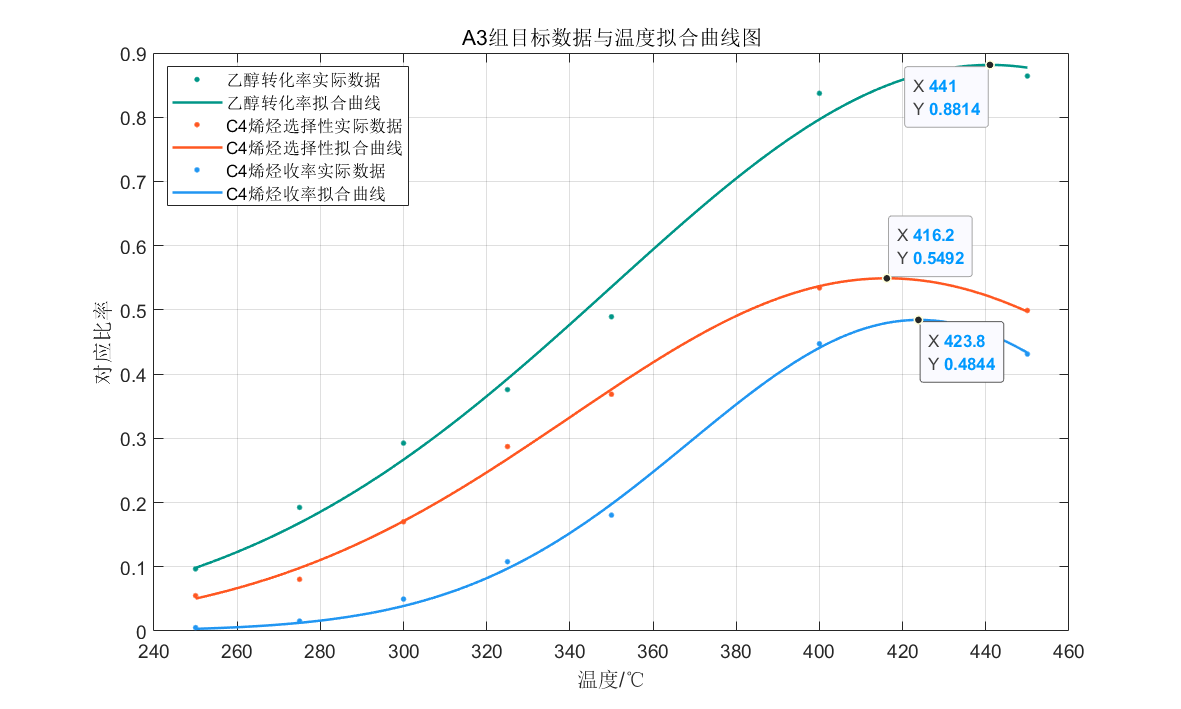
\includegraphics[width=.9\textwidth]{A3}
	\caption{A3 Gauss Model }
	\label{fig:B7}
\end{figure}

\newpage
从图1中可以看出:
\begin{itemize}
	\item 乙醇转化率与温度基本符合高斯曲线。在该种催化剂组合的条件下,当温度降低时,乙醇转化率随着温度的升高而增大;当温度为441度时,乙醇转化率达到最大值88.14\%之后,随着温度的升高而逐渐降低。
	\item C4烯烃选择性与温度基本符合高斯曲线。在该种催化剂组合的条件下,当温度降低时,C4烯烃选择性随着温度的升高而增大;当温度为416.2度时,C4烯烃选择性达到最大,为54.92\%;之后,随着温度的升高而逐渐降低。
	\item C4烯烃收率与温度基本符合高斯曲线。在该种催化剂组合的条件下,当温度降低时,C4烯烃收率随着温度的升高而增大;当温度为423.8度时,C4烯烃收率达到最大值48.44\%之后,随着温度的升高而逐渐降低。
\end{itemize}

\begin{table}[!htbp]
	\caption{A3组待估计参数值}\label{tab:001} \centering
	\begin{tabular}{cccc}
		\toprule[1.5pt]
		函数& a & b & c \\
		\midrule[1pt]
		温度-乙醇转化率 & 0.8814  (0.7965, 0.9664) & 441  (410.6, 471.4) & 129  (97.95, 160)\\
		温度-C4烯烃选择性 & 0.5491  (0.5196, 0.5787) & 416.1  (407.5, 424.8) & 107.6  (96.41, 118.7) \\
		温度-C4烯烃收率 & 0.4844  (0.4544, 0.5144) & 423.9  (417.7, 430.2)& 78.06  (69.89, 86.22)\\
		\bottomrule[1.5pt]
	\end{tabular}
\end{table}

同时,我们给出在置信度为95\%时,高斯曲线中待估计参数以及对应的置信区间(表2):从表中可以看出,参数b所代表的含义时高斯曲线的峰值所在位置,这与图1中的数据相符。对应的置信区间有助于我们在现实实验中在该催化剂组合下寻找最优温度。

为了评估拟合的效果,我们计算了有关拟合优度的评估指标(表3):从表中可以看出,三组拟合曲线的和方差(SSE)均小于0.008,确定系数(R-square)均大于0.98,标准差(RMSE)也均小于0.038,这说明我们的方案具有较高的拟合效果,进一步证明了温度与乙醇转化率、C4烯烃选择性的高斯函数关系是可靠的。

\begin{table}[!htbp]
	\caption{A3组拟合优度}\label{tab:001} \centering
	\begin{tabular}{ccccc}
		\toprule[1.5pt]
		函数& SSE & R-square & Adjusted R-square & RMSE \\
		\midrule[1pt]
		温度-乙醇转化率 &  0.005489 & 0.9899 & 0.9849 &   0.03704\\
		温度-C4烯烃选择性 &  0.0007808 & 0.9965 &  0.9947 & 0.01397 \\
		温度-C4烯烃收率 & 0.0005836 & 0.9973&  0.9959 & 0.01208\\
		\bottomrule[1.5pt]
	\end{tabular}
\end{table}

经整体分析,其余20组的实验结果与A3组的情况基本符合,有些组由于实验数据中并未达到最优解,所以在拟合曲线中没有出现峰值。每一组的拟合曲线图如下所示,而每组对应的带估计参数和拟合优度表详见“我的支撑材料-问题1\_温度关系.docx”文件。

\begin{figure}[!h]
	\centering
	\begin{minipage}[c]{0.45\textwidth}
		\centering
		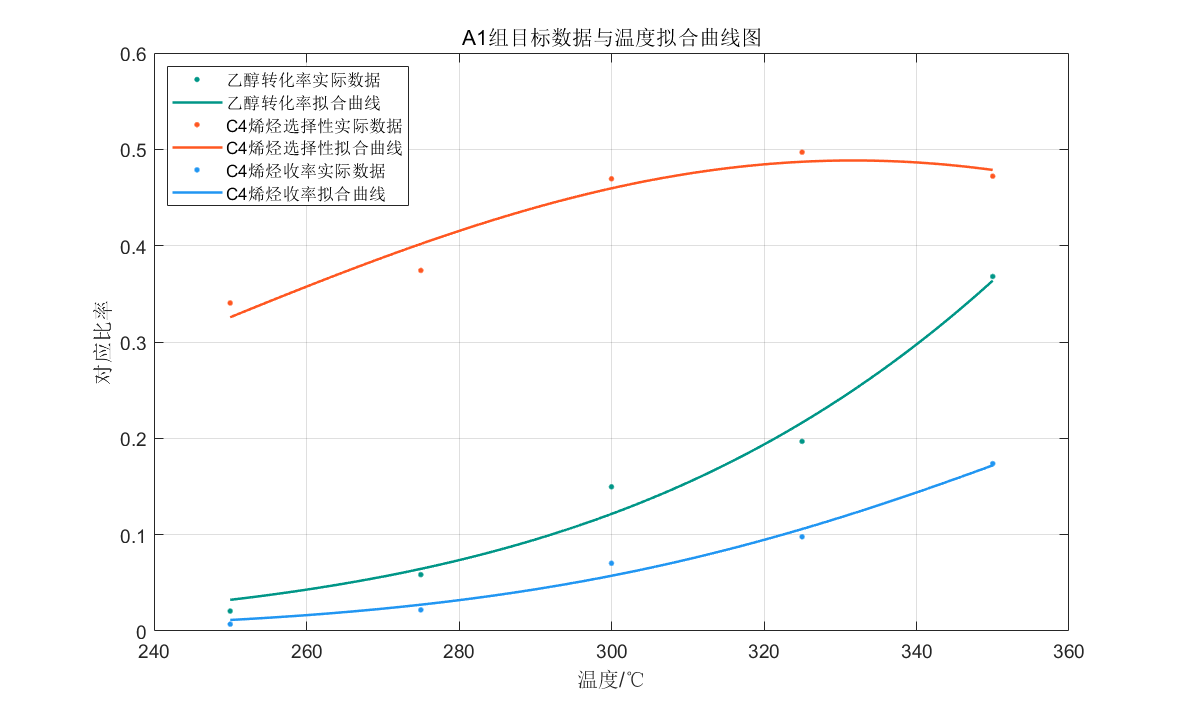
\includegraphics[width=0.95\textwidth]{A1}
		\subcaption{A1 Gauss Model}
		\label{fig:sample-figure-a}
	\end{minipage}
	\begin{minipage}[c]{0.45\textwidth}
		\centering
		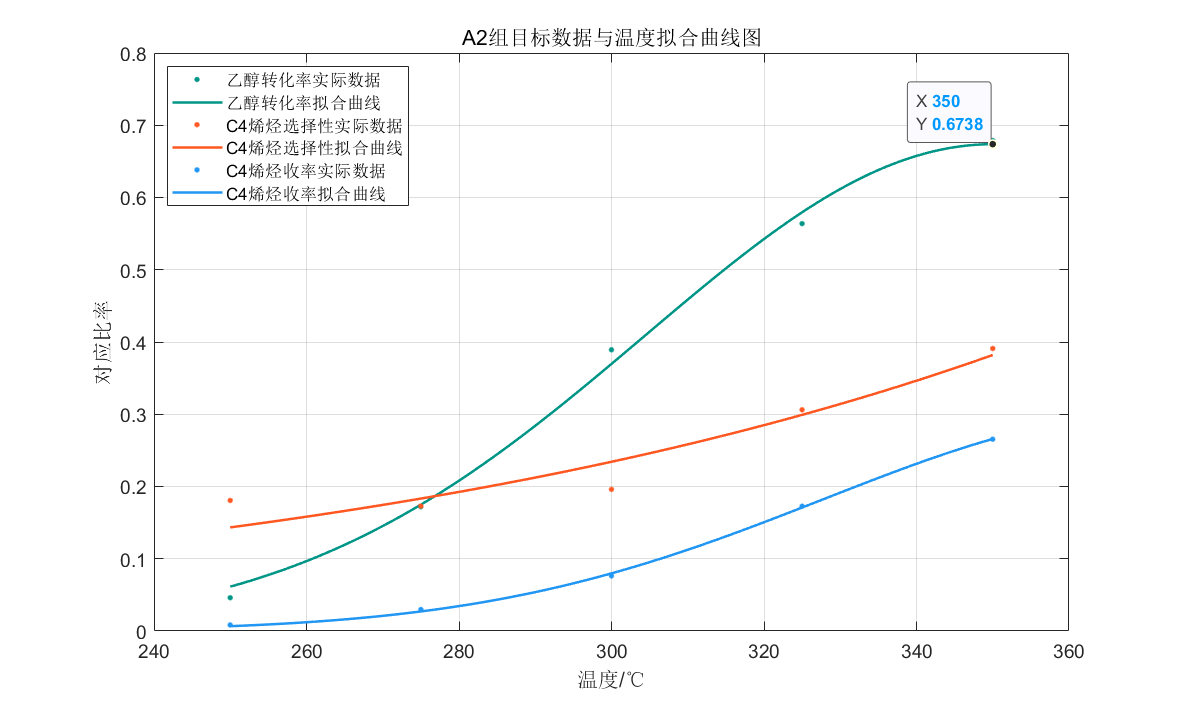
\includegraphics[width=0.95\textwidth]{A2}
		\subcaption{A2 Gauss Model}
		\label{fig:sample-figure-b}
	\end{minipage}
	\caption{A1-2 Gauss Model}
	\label{fig:sample-figure}
\end{figure}

\newpage
\begin{figure}[!h]
	\centering
	\begin{minipage}[c]{0.45\textwidth}
		\centering
		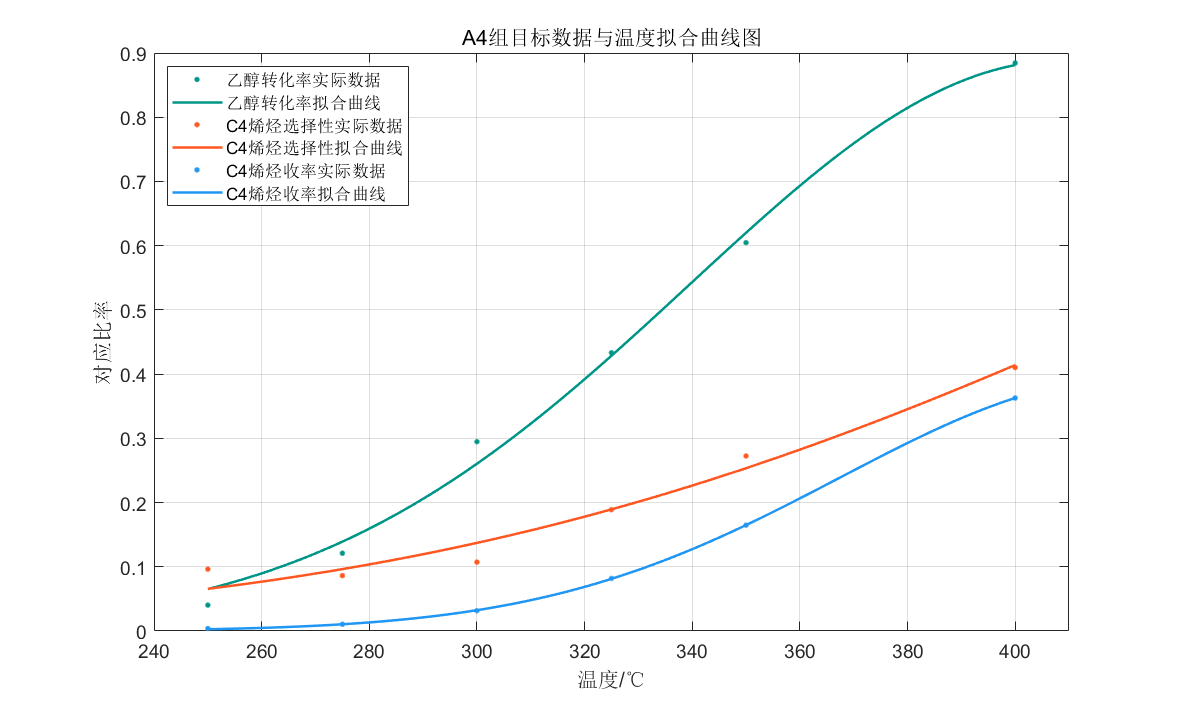
\includegraphics[width=0.95\textwidth]{A4}
		\subcaption{A4 Gauss Model}
		\label{fig:sample-figure-a}
	\end{minipage}
	\begin{minipage}[c]{0.45\textwidth}
		\centering
		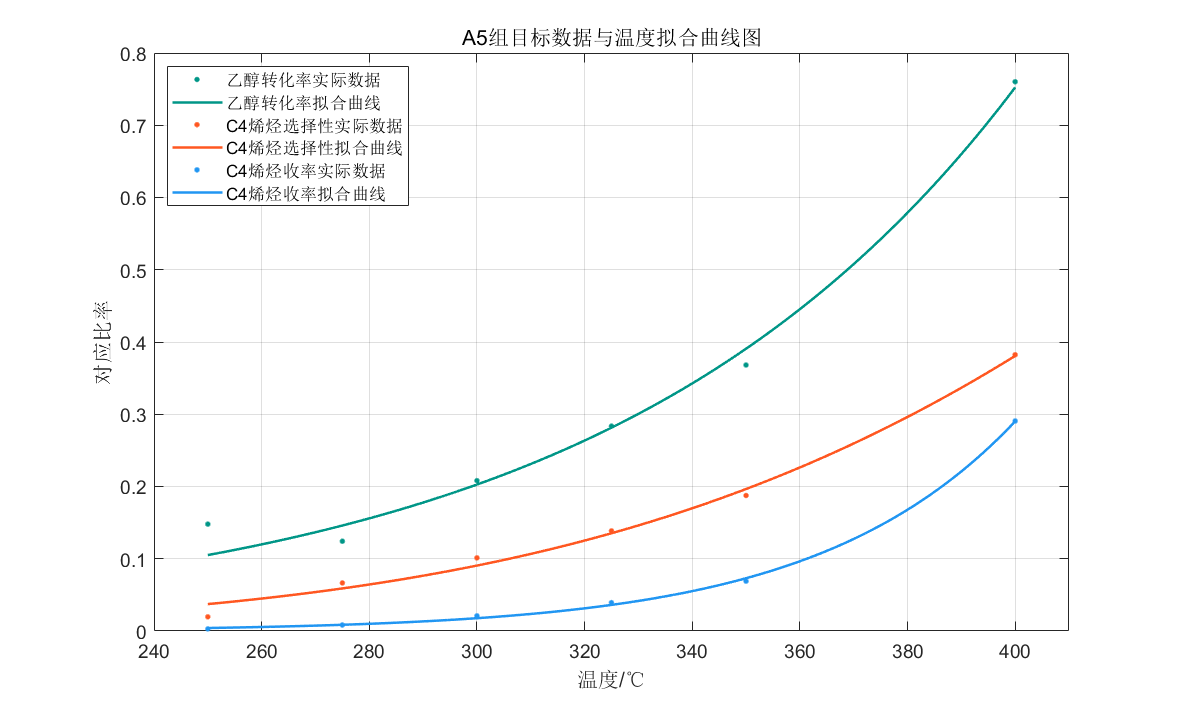
\includegraphics[width=0.95\textwidth]{A5}
		\subcaption{A5 Gauss Model}
		\label{fig:sample-figure-b}
	\end{minipage}
	\caption{A4-5 Gauss Model}
	\label{fig:sample-figure}
\end{figure}

\begin{figure}[!h]
	\centering
	\begin{minipage}[c]{0.45\textwidth}
		\centering
		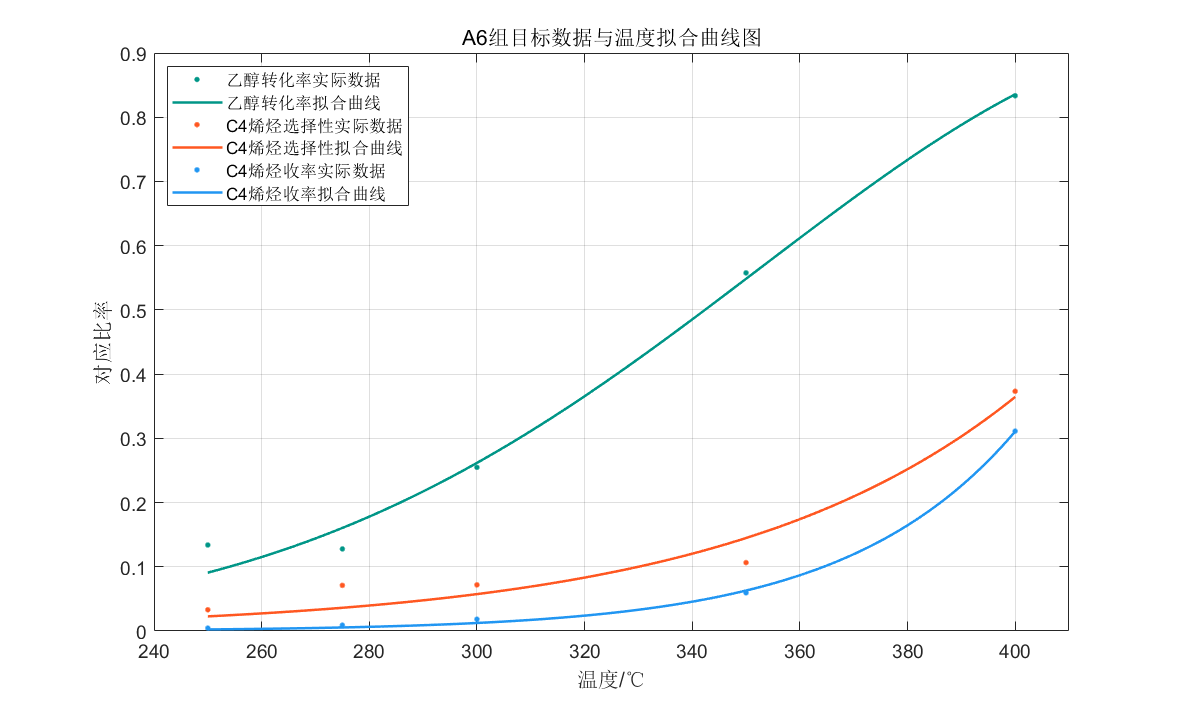
\includegraphics[width=0.95\textwidth]{A6}
		\subcaption{A6 Gauss Model}
		\label{fig:sample-figure-a}
	\end{minipage}
	\begin{minipage}[c]{0.45\textwidth}
		\centering
		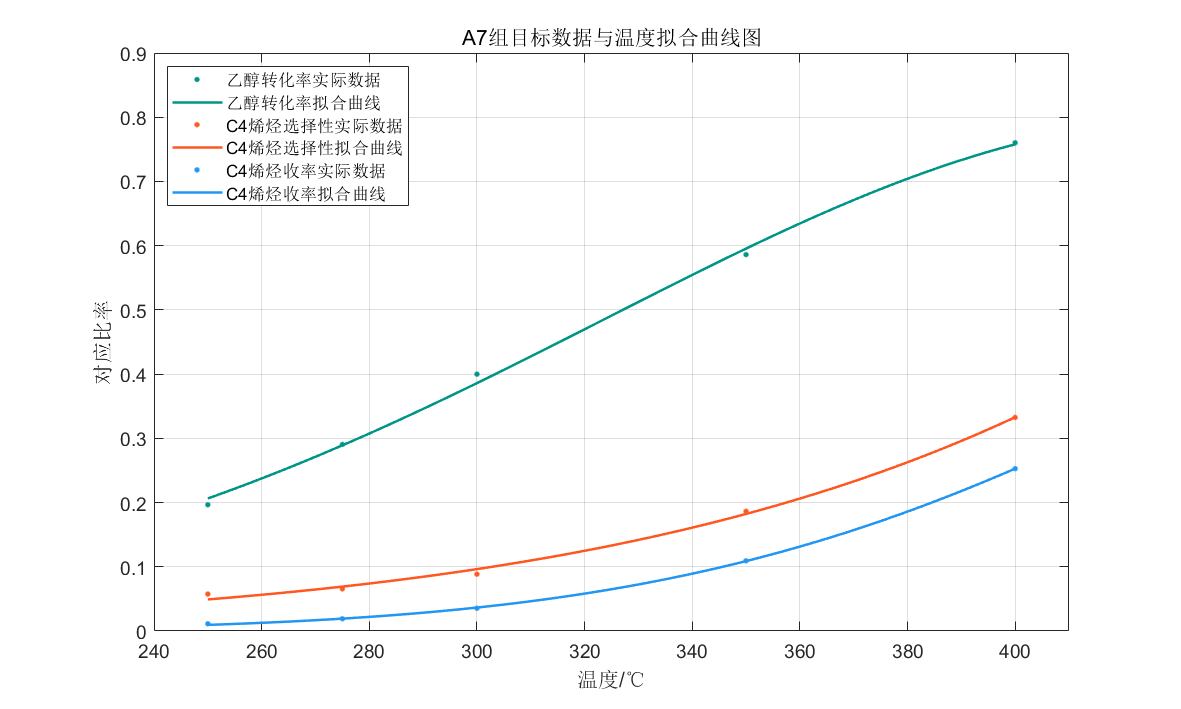
\includegraphics[width=0.95\textwidth]{A7}
		\subcaption{A7 Gauss Model}
		\label{fig:sample-figure-b}
	\end{minipage}
	\caption{A6-7 Gauss Model}
	\label{fig:sample-figure}
\end{figure}

\begin{figure}[!h]
	\centering
	\begin{minipage}[c]{0.45\textwidth}
		\centering
		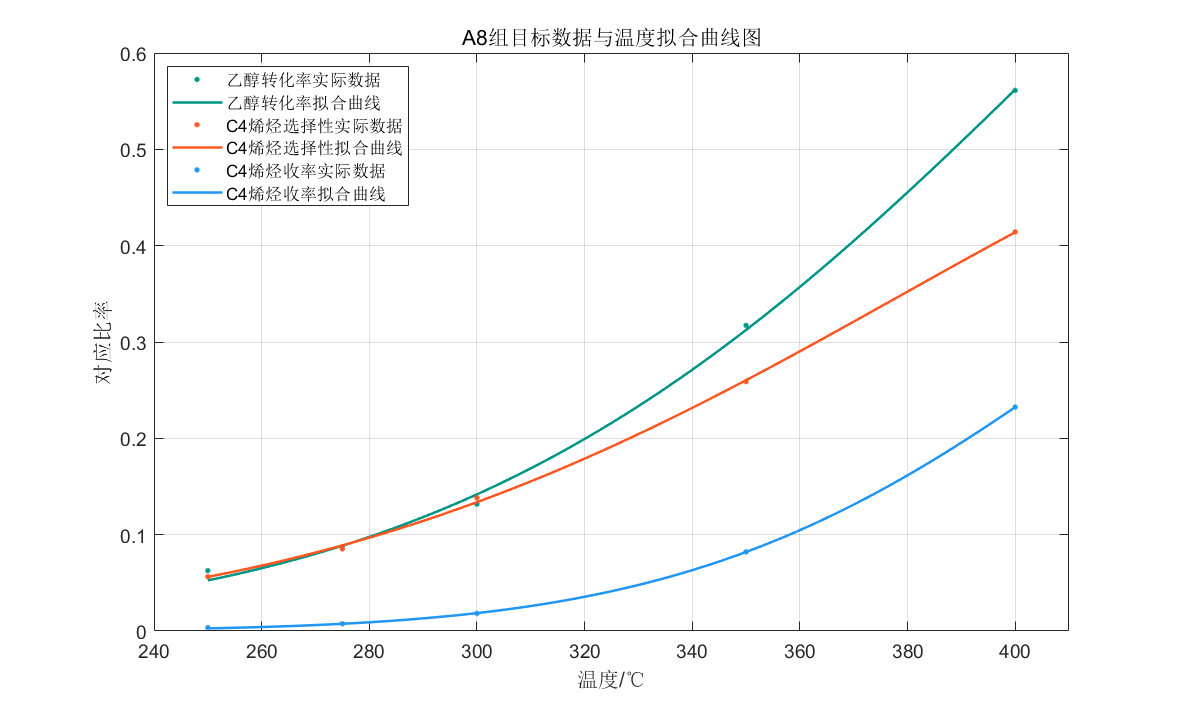
\includegraphics[width=0.95\textwidth]{A8}
		\subcaption{A8 Gauss Model}
		\label{fig:sample-figure-a}
	\end{minipage}
	\begin{minipage}[c]{0.45\textwidth}
		\centering
		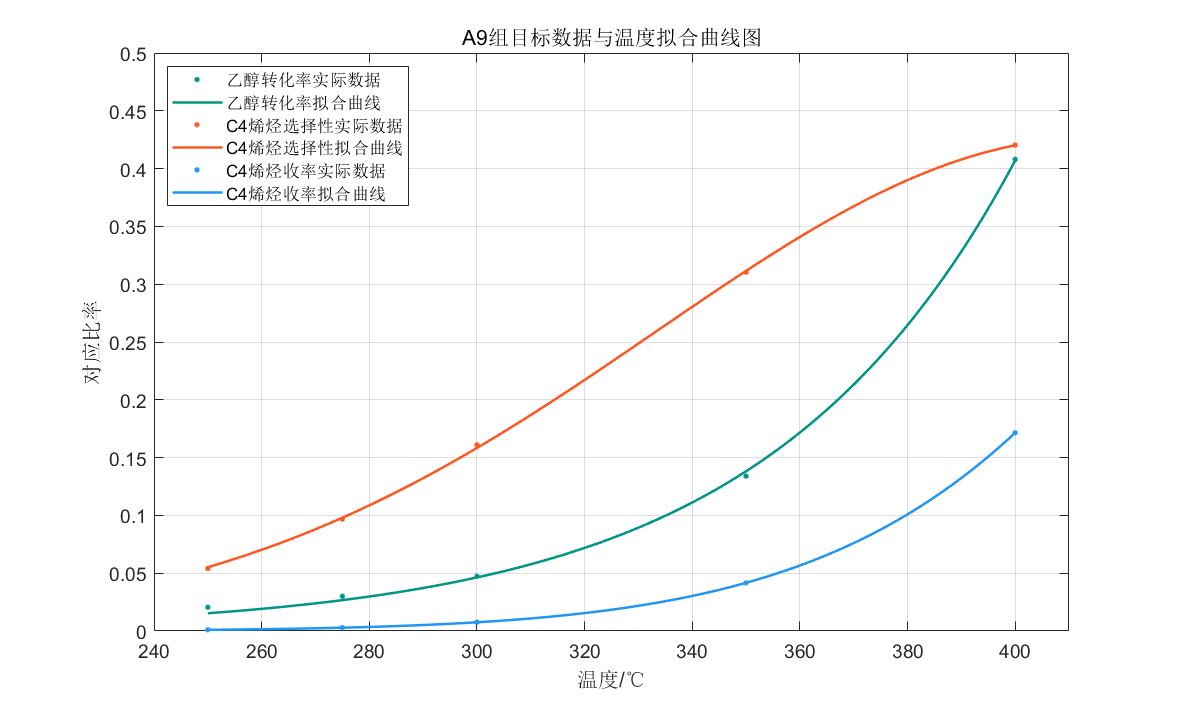
\includegraphics[width=0.95\textwidth]{A9}
		\subcaption{A9 Gauss Model}
		\label{fig:sample-figure-b}
	\end{minipage}
	\caption{A8-9 Gauss Model}
	\label{fig:sample-figure}
\end{figure}


\newpage
\begin{figure}[!h]
	\centering
	\begin{minipage}[c]{0.45\textwidth}
		\centering
		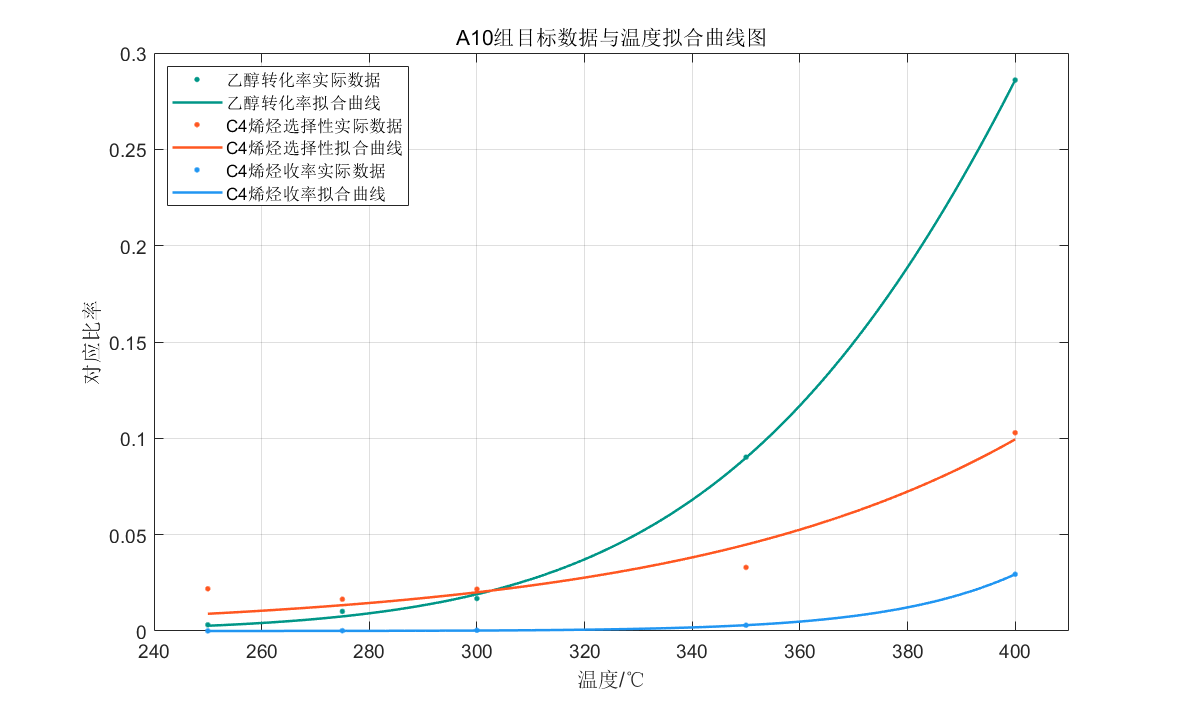
\includegraphics[width=0.95\textwidth]{A10}
		\subcaption{A10 Gauss Model}
		\label{fig:sample-figure-a}
	\end{minipage}
	\begin{minipage}[c]{0.45\textwidth}
		\centering
		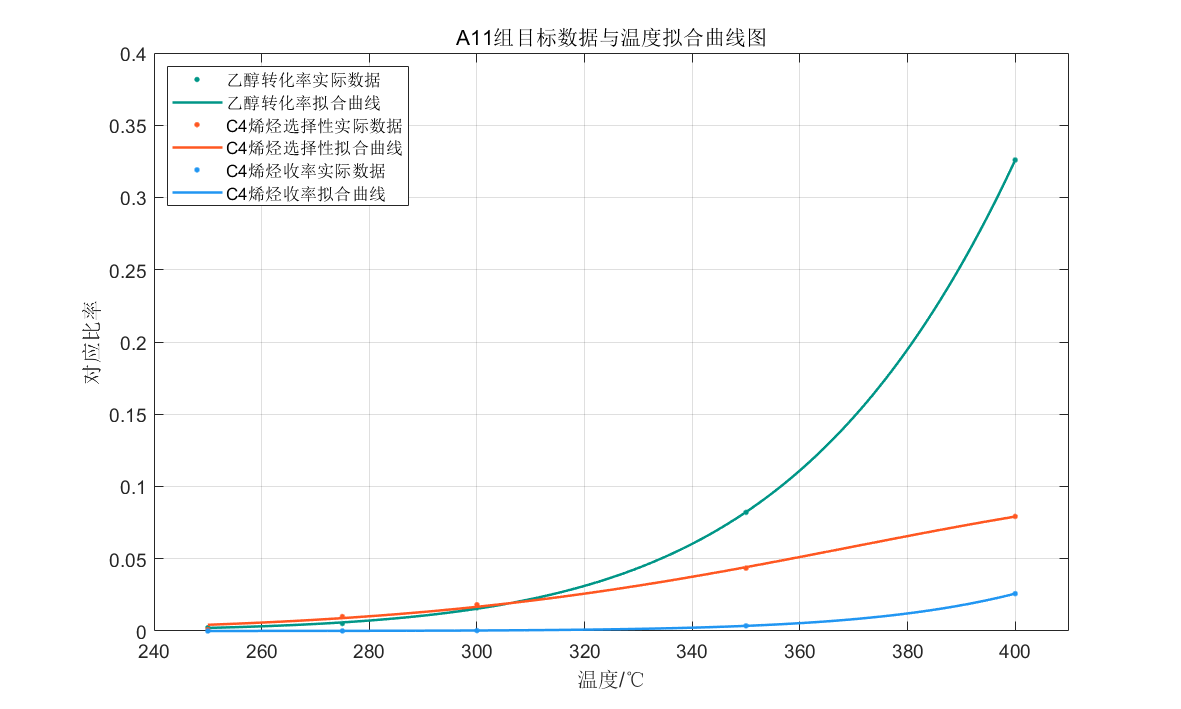
\includegraphics[width=0.95\textwidth]{A11}
		\subcaption{A11 Gauss Model}
		\label{fig:sample-figure-b}
	\end{minipage}
	\caption{A10-11 Gauss Model}
	\label{fig:sample-figure}
\end{figure}

\begin{figure}[!h]
	\centering
	\begin{minipage}[c]{0.45\textwidth}
		\centering
		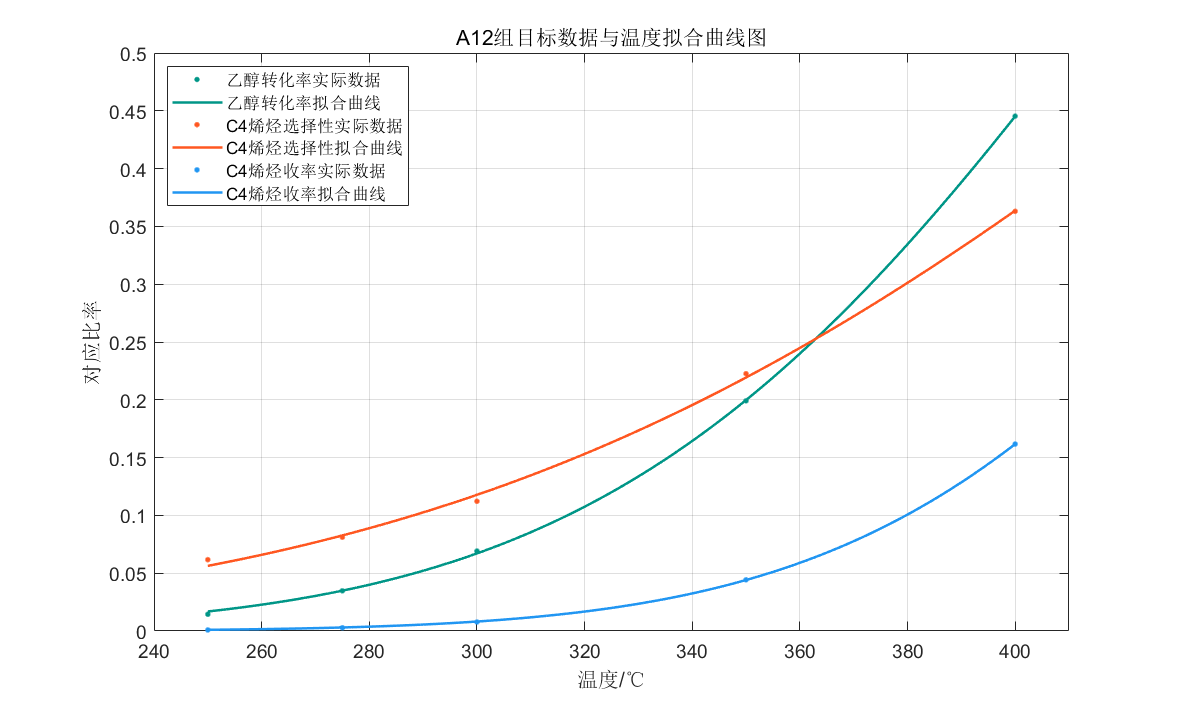
\includegraphics[width=0.95\textwidth]{A12}
		\subcaption{A12 Gauss Model}
		\label{fig:sample-figure-a}
	\end{minipage}
	\begin{minipage}[c]{0.45\textwidth}
		\centering
		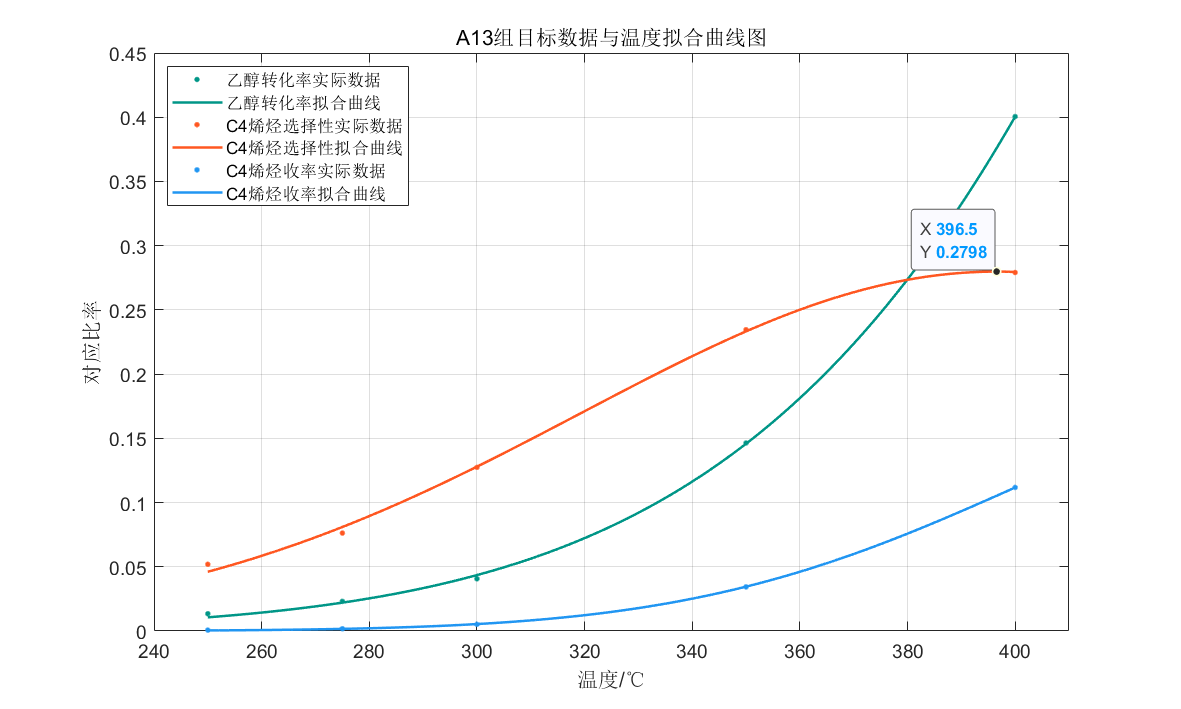
\includegraphics[width=0.95\textwidth]{A13}
		\subcaption{A13 Gauss Model}
		\label{fig:sample-figure-b}
	\end{minipage}
	\caption{A12-13 Gauss Model}
	\label{fig:sample-figure}
\end{figure}

\begin{figure}[!h]
	\centering
	\begin{minipage}[c]{0.45\textwidth}
		\centering
		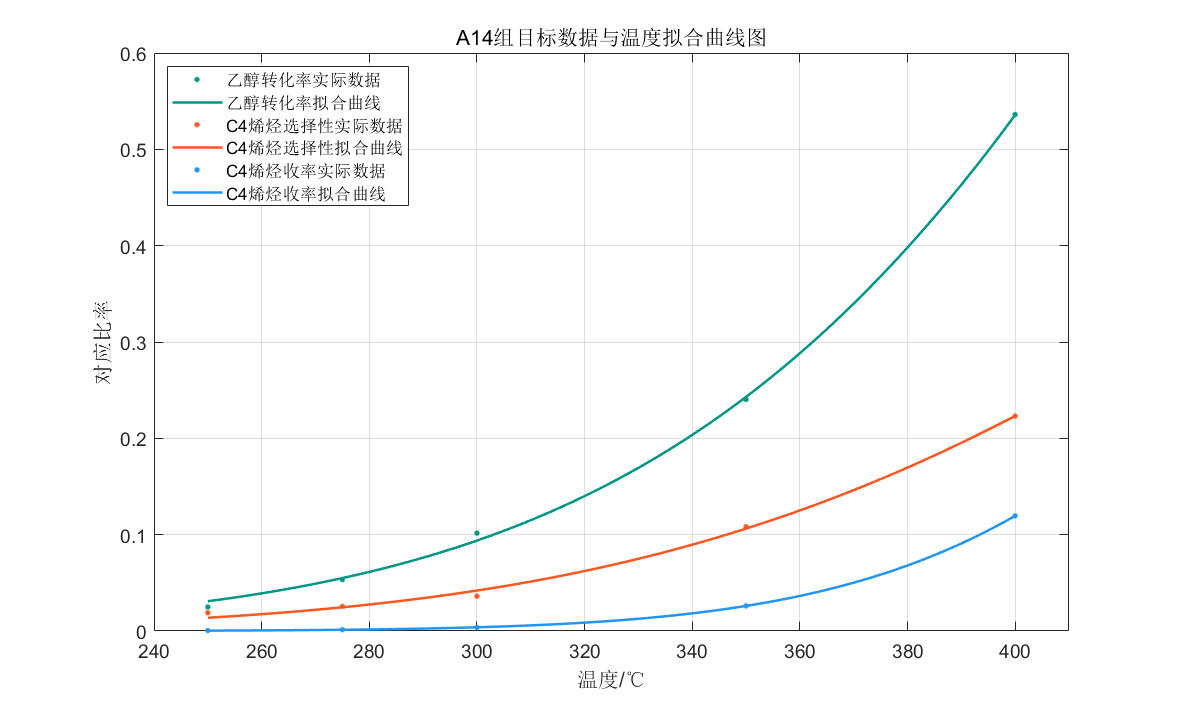
\includegraphics[width=0.95\textwidth]{A14}
		\subcaption{A14 Gauss Model}
		\label{fig:sample-figure-a}
	\end{minipage}
	\begin{minipage}[c]{0.45\textwidth}
		\centering
		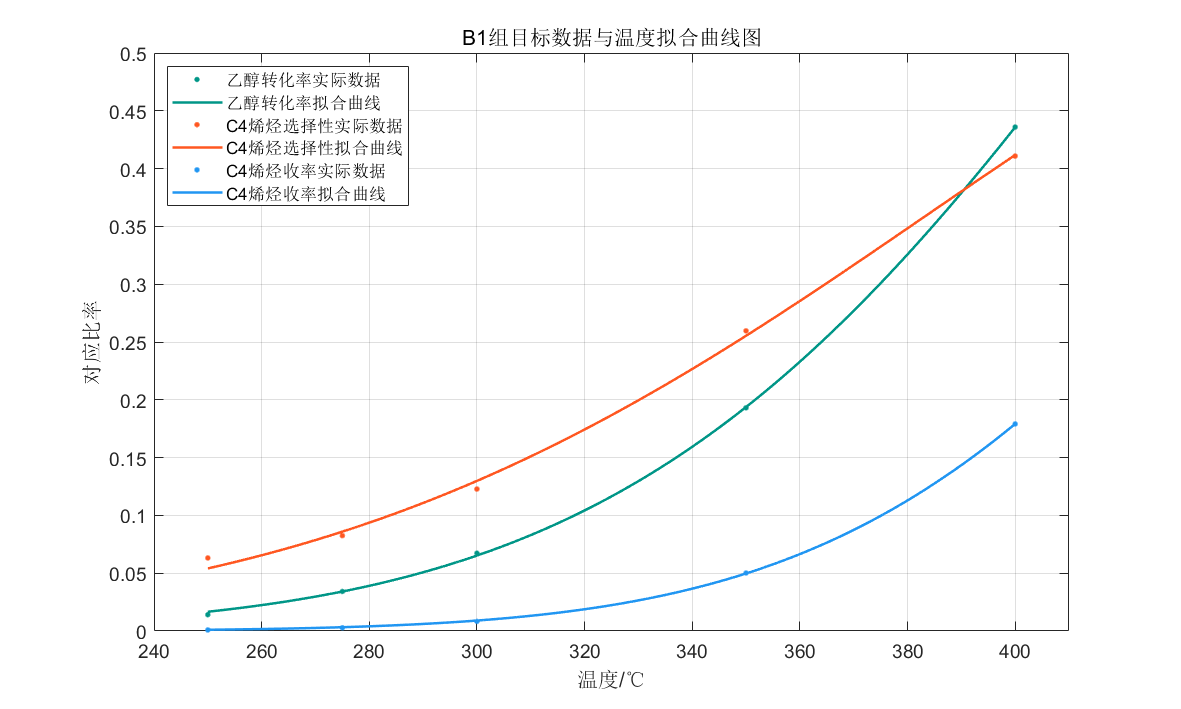
\includegraphics[width=0.95\textwidth]{B1}
		\subcaption{B1 Gauss Model}
		\label{fig:sample-figure-b}
	\end{minipage}
	\caption{A14-B1 Gauss Model}
	\label{fig:sample-figure}
\end{figure}


\begin{figure}[!h]
	\centering
	\begin{minipage}[c]{0.45\textwidth}
		\centering
		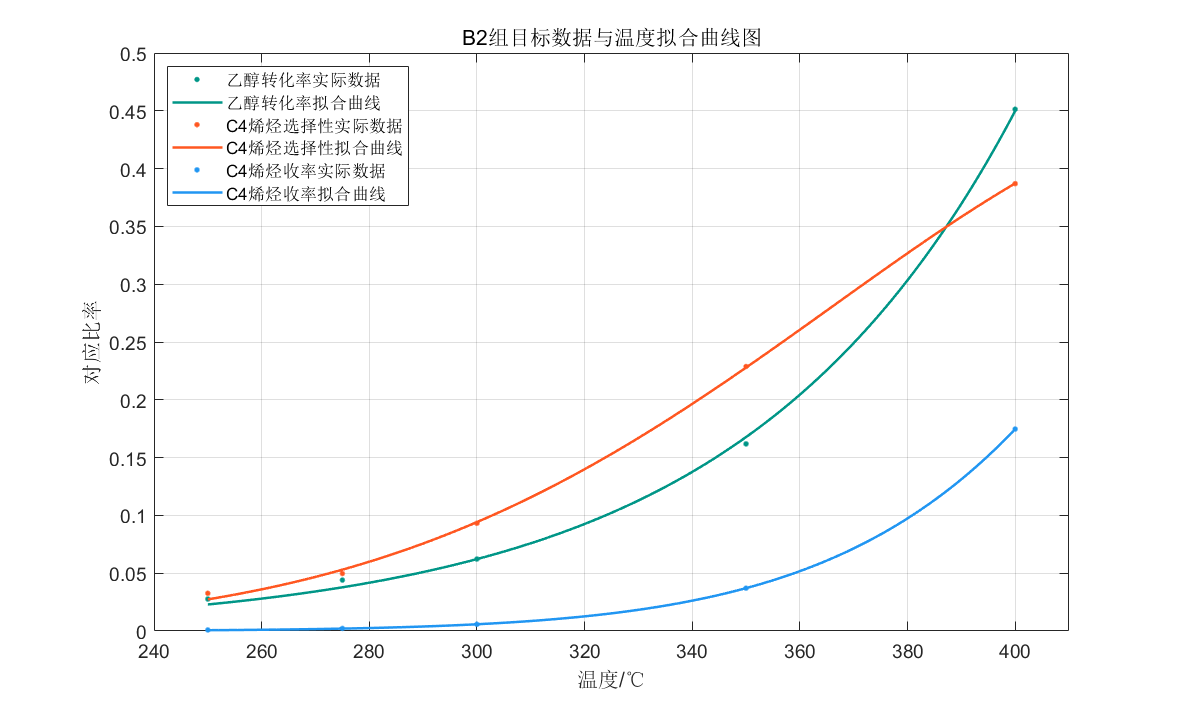
\includegraphics[width=0.95\textwidth]{B2}
		\subcaption{B2 Gauss Model}
		\label{fig:sample-figure-a}
	\end{minipage}
	\begin{minipage}[c]{0.45\textwidth}
		\centering
		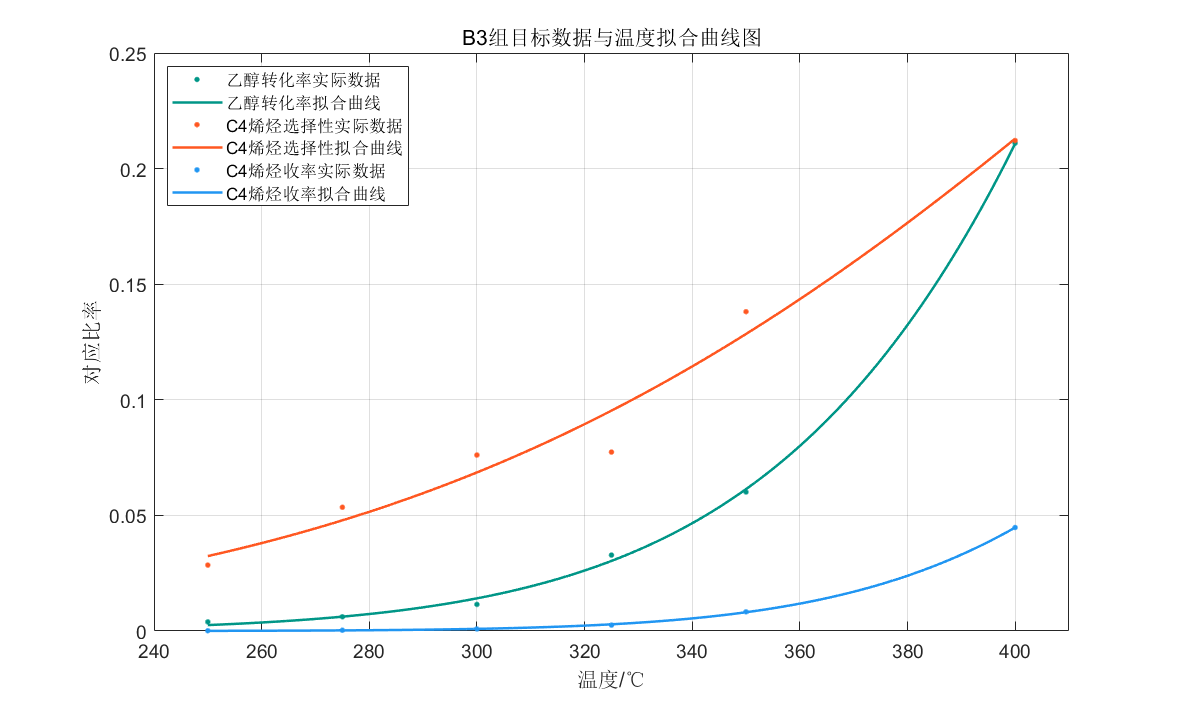
\includegraphics[width=0.95\textwidth]{B3}
		\subcaption{B3 Gauss Model}
		\label{fig:sample-figure-b}
	\end{minipage}
	\caption{B2-3 Gauss Model}
	\label{fig:sample-figure}
\end{figure}

\newpage

\begin{figure}[!h]
	\centering
	\begin{minipage}[c]{0.45\textwidth}
		\centering
		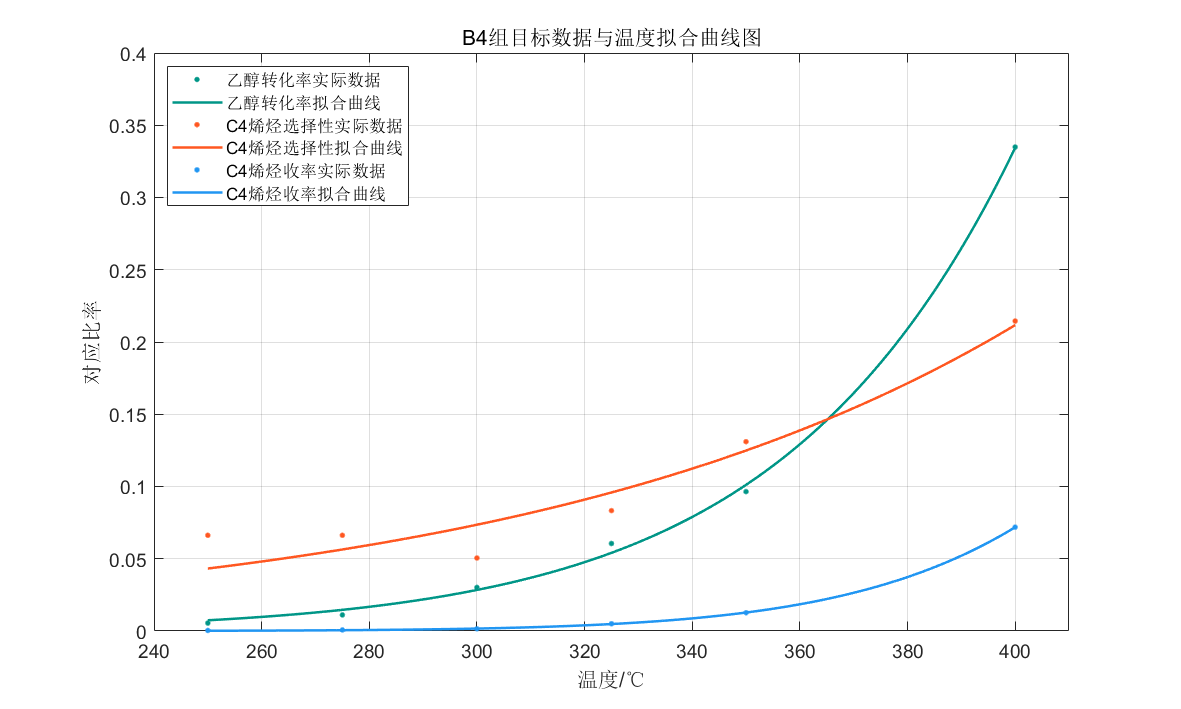
\includegraphics[width=0.95\textwidth]{B4}
		\subcaption{B4 Gauss Model}
		\label{fig:sample-figure-a}
	\end{minipage}
	\begin{minipage}[c]{0.45\textwidth}
		\centering
		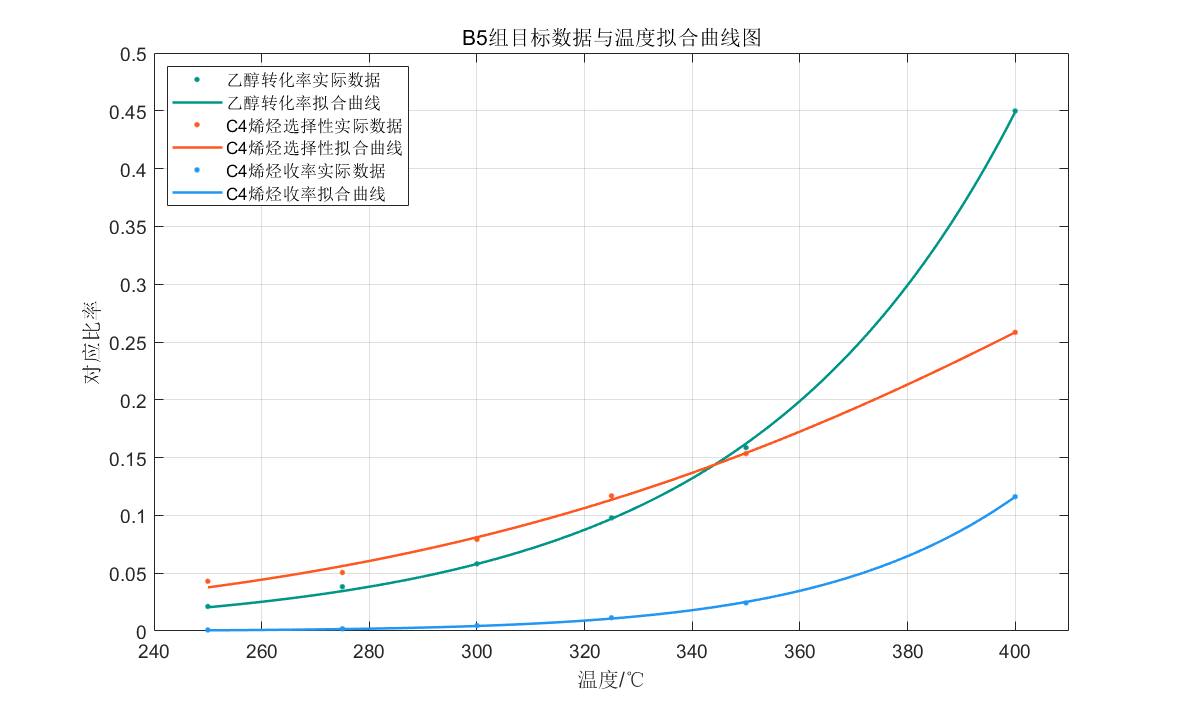
\includegraphics[width=0.95\textwidth]{B5}
		\subcaption{B5 Gauss Model}
		\label{fig:sample-figure-b}
	\end{minipage}
	\caption{B4-5 Gauss Model}
	\label{fig:sample-figure}
\end{figure}

\begin{figure}[!h]
	\centering
	\begin{minipage}[c]{0.45\textwidth}
		\centering
		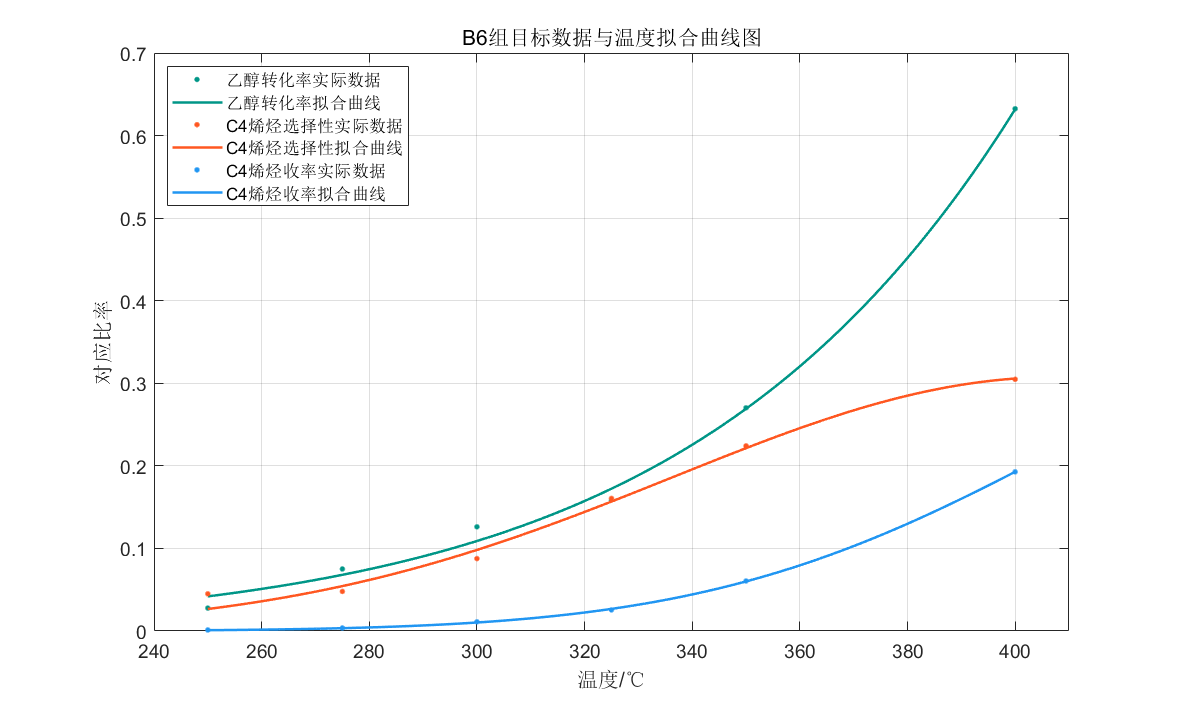
\includegraphics[width=0.95\textwidth]{B6}
		\subcaption{B6 Gauss Model}
		\label{fig:sample-figure-a}
	\end{minipage}
	\begin{minipage}[c]{0.45\textwidth}
		\centering
		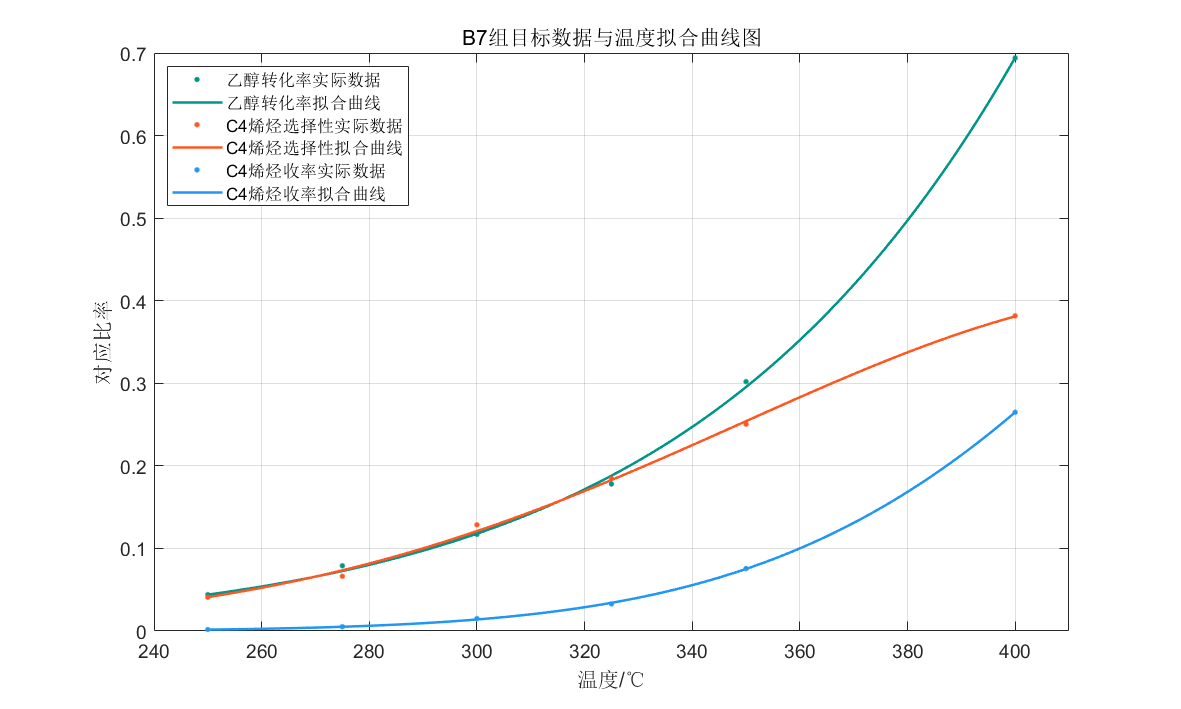
\includegraphics[width=0.95\textwidth]{B7}
		\subcaption{B7 Gauss Model}
		\label{fig:sample-figure-b}
	\end{minipage}
	\caption{B6-7 Gauss Model}
	\label{fig:sample-figure}
\end{figure}


\newpage
\subsubsection{附件2结果分析}
借助matlab中的cftool工具包,我们基于指数模型$\ \ x(t)\ =\ a\ast(exp(-(t-b)/e))+d$对乙醇转化率与时间的关系进行拟合,结果如图12.

% 插入单张图片
\begin{figure}[!h]
	\centering
	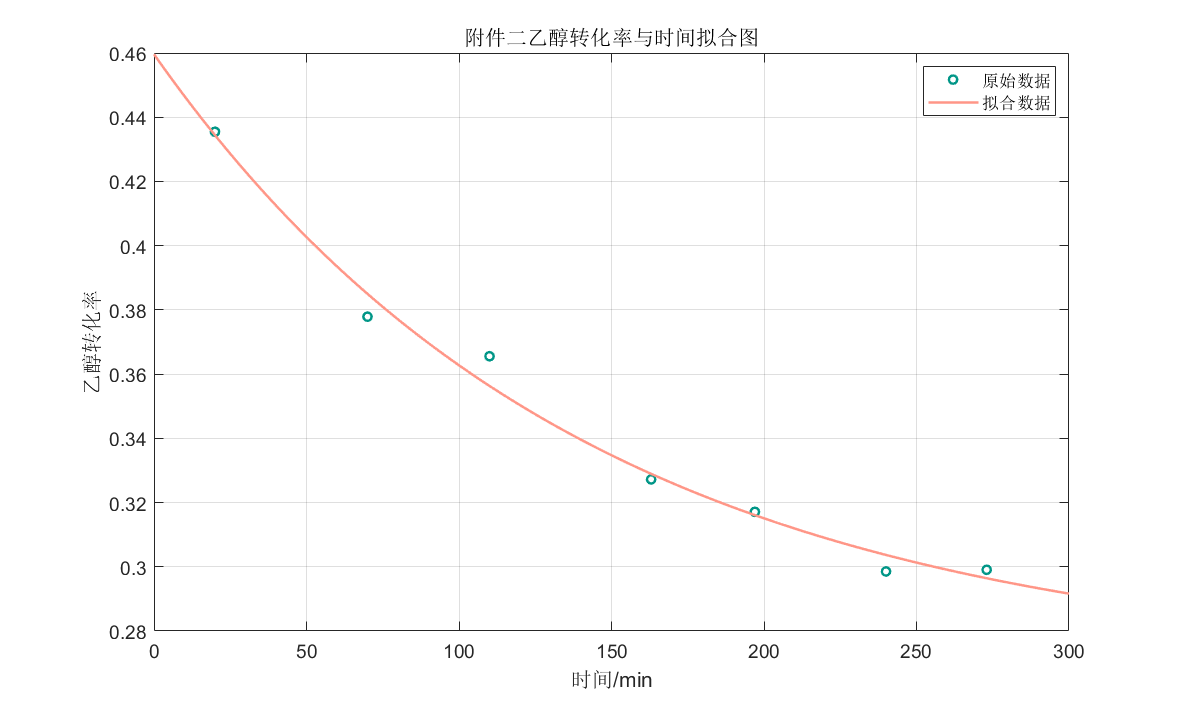
\includegraphics[width=1.0\textwidth]{x_t}
	\caption{乙醇转化率与时间拟合图}
	\label{fig:circuit-diagram}
\end{figure}
拟合结果在95\%的置信度下的待估计参数值分别为$a = 0.1655  (-1.125e+05, 1.125e+05), b = 20  (-9.59e+07, 9.59e+07), e = 141  (19.47, 262.5),  d = 0.2689  (0.2036, 0.3343)$。拟合优度相关参数为:  $SSE = 0.0001745, R-square = 0.9884 ,Adjusted R-square =  0.9768, RMSE = 0.007626$。

在$x(t)$的基础上,我们可以得到(7)式中$\frac{v}{c}$的函数图像(图13):
\begin{figure}[!h]
	\centering
	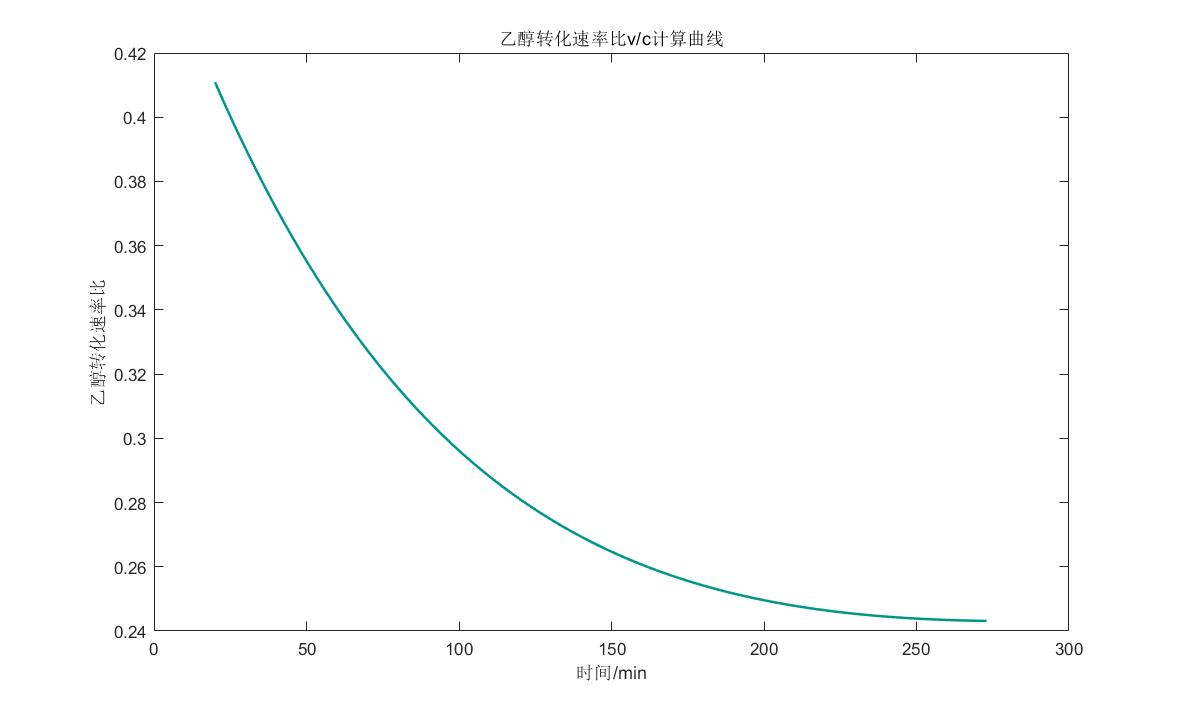
\includegraphics[width=0.8\textwidth]{v_c}
	\caption{乙醇转化速率比v/c计算曲线}
	\label{fig:circuit-diagram1}
\end{figure}

在经过量纲分析法处理后,为了简化(8)式,我们根据模型(7)式计算出附加二表格对应C4烯烃选择性的$\frac{v}{c}$(表4):
\begin{table}[!htbp]
	\caption{C4烯烃选择性y的乙醇转化速率比$\frac{v}{c}$}\label{tab:001} \centering
	\begin{tabular}{cccccccc}
		\toprule[1.5pt]
		时间(min)& 20 & 70 & 110 & 163 & 197 & 240 & 273 \\
		\midrule[1pt]
		$y$ & 39.9 & 38.55 & 36.72 & 39.53 & 38.96 & 40.32 & 39.04 \\
		$\frac{v}{c}$& 0.4109 & 0.3274 & 0.2881 & 0.2595 & 0.2502 & 0.2445 & 0.2431 \\
		\bottomrule[1.5pt]
	\end{tabular}
\end{table}

\begin{figure}[!h]
	\centering
	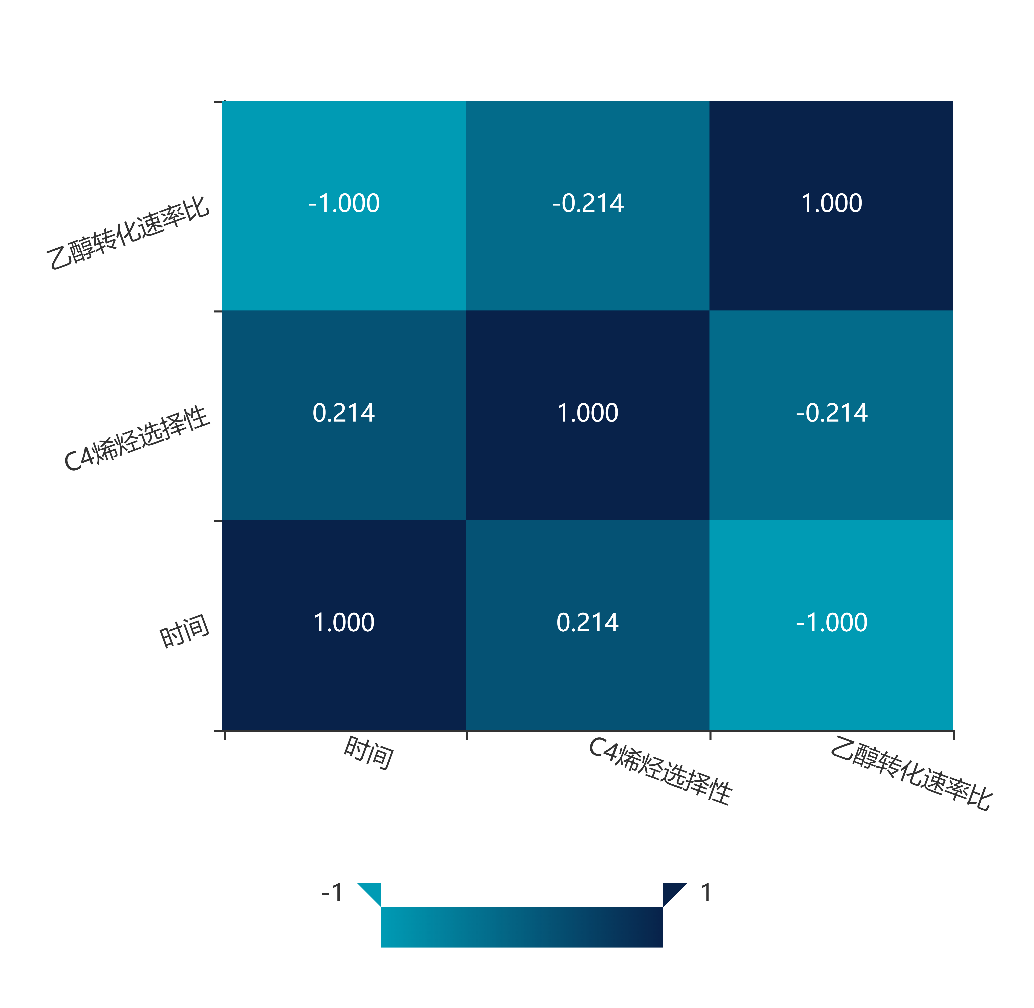
\includegraphics[width=0.8\textwidth]{spe}
	\caption{Spearman相关系数}
	\label{fig:circuit-diagram1}
\end{figure}

对表4中的变量进行Spearman相关系数分析(图14):乙醇转化速率比($\frac{v}{c}$)与C4烯烃选择性($y$)之间的Spearman相关系数只有-0.214,可以认为二者并没有紧密的相关关系,基于此,我们可以将(7)式中的y当作常因子进行处理:
\begin{equation*}
	\frac{v}{c}=\left(\frac{k1\ast\left(1-x\right)}{k2\ast x}\right)^{k6}+\left(\frac{k3\ast\left(1-x\right)}{k4\ast x}\right)^{k7}+k5
\end{equation*}

进一步化简处理,可以发现模型最终可以表示为一个多项式的形式:

\begin{equation*}
	\frac{v}{c}=k0+k1\ast x+k2\ast x^2+k3\ast x^3\ldots
\end{equation*}

由上分析可知,v/c与乙醇转化率的关系较为密切,而与C4烯烃选择性的关系不大,并且可以采用多项式拟合的方法对于$\frac{v}{c}$进行拟合,经过实验对比,采用二次函数拟合便可以较好地进行。即使用二次函数:$v/c\ =\ p1\ast x^2\ +\ p2\ast x\ +\ p3$进行拟合。拟合结果图如下:
\begin{figure}[!h]
	\centering
	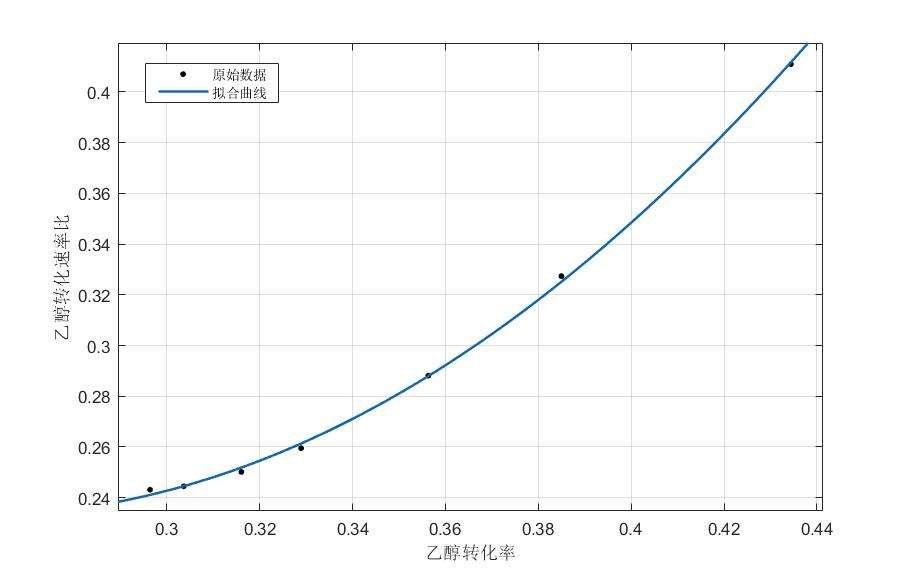
\includegraphics[width=1.0\textwidth]{1_end}
	\caption{乙醇转化率比与乙醇转化率函数关系}
	\label{fig:circuit-diagram1}
\end{figure}
在置信度为95\%的条件下,二次函数系数分别为:$ p1 =       5.815  (4.673, 6.957),
p2 =      -3.013  (-3.845, -2.182),
p3 =      0.6234  (0.4743, 0.7724),
 $。拟合优度相关指标分别为:$ SSE = 1.586e-05
 R-square= 0.9993,
 Adjusted R-square= 0.999,
 RMSE: 0.001991
 $
 
综上所述,得到以下结论:

\begin{enumerate}
	\item 随着时间的推移,乙醇转化率呈下降趋势,并且下降趋势呈现指数趋势,指数方程为$x(t)\ =\ 0.1655\ast(exp(-(t-20)/141))+0.2689$.
	\item 根据图1,可以说明C4烯烃选择性和时间无密切相关关系,乙醇转化速率比和C4烯烃选择性无密切相关关系,而乙醇转化速率比和时间存在密切相关关系,也侧面证明了采用曲线拟合的合理性。
	
	\item 随着时间的推移,乙醇转化速率(和乙醇转化速率比趋势相同)呈下降趋势,并且下降趋势呈现指数趋势,乙醇转化速率比的指数方程为$\frac{v}{c}=x(t)+t\ast\frac{dx(t)}{dt}$.
	
	\item 由于C4烯烃选择性和其他产物的选择性为互补关系,而C4烯烃选择性和时间无密切相关关系,因此可以认为其他产物的选择性和时间无密切相关关系。
	
	\item 乙醇转化速率与乙醇转化率之间的关系使用多项式拟合方法描述更佳,其拟合方程为:$\frac{v}{c}\ =\ 5.815\ast x^2\ -3.013\ast x\ +\ 0.6234$.	
\end{enumerate}


\section{问题二的模型建立与求解}
\subsection{问题的分析}
思路一是采用控制变量法,从众多实验数据中寻找相互对照的组合,当某一个指标发生变化,而其它指标保持不变,探究乙醇转化率以及 C4 烯烃选择性的变化。催化剂展开为Co负载量、Co/SiO2 和 HAP装料比、Co/SiO2 和 HAP的质量总和、乙醇浓度四个变量。

思路二是对催化剂组合和温度对因变量共同作用所产生的影响,我们将采用权重分析法定性分析催化剂中各因素对因变量的影响权重。


\subsection{单因素模型的建立与求解}
\subsubsection{乙醇转化率与催化剂组合关系}
\textbf{乙醇转化率 -- Co/SiO2和HAP装料比}

通过观察实验数据可以发现,A12,A13,A14是关于o/SiO2和HAP装料比的对照组,我们通过原型函数$ f(x) = a*exp(-b*x)+c$对乙醇转化率与装料比的关系进行拟合,根据图像可以看出有很好的拟合效果。
\begin{figure}[!h]
	\centering
	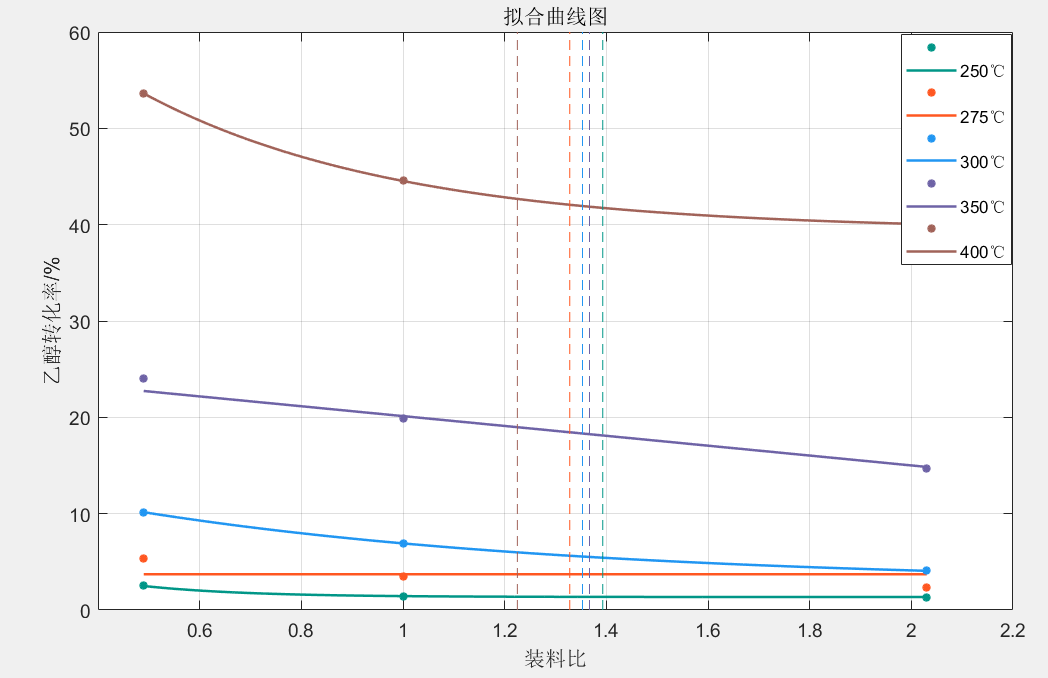
\includegraphics[width=1.0\textwidth]{2_9}
	\caption{乙醇转化率 -- Co/SiO2和HAP装料比拟合曲线}
	\label{fig:circuit-diagram1}
\end{figure}
待估计参数为(表5):
\begin{table}[!htbp]
	\caption{乙醇转化率与装料比待估计参数}\label{tab:001} \centering
	\begin{tabular}{cccc}
		\toprule[1.5pt]
		温度(°C) & a & b & c \\
		\midrule[1pt]
		250 & 12.5 &   4.875 &  1.346\\
		275 & -56.19 &   103.2 & 3.705 \\
		300 &12.85 & 1.135&  2.783 \\
		350 &-2289 &  -0.002229& 2315  \\
		400 & 37.79  &   1.993 & 39.39 \\
		\bottomrule[1.5pt]
	\end{tabular}
\end{table}
\newpage
根据图表(图16)分析可得:
\begin{itemize}
	\item 基于化学反应机理可知:Co/SiO2 和 HAP同为反应的催化剂,在达到合适的比例的情况下能实现更高的转化率,而某一方如果占比过多会相对不利于反应的进行,故从原理上应该是先增加后减少的趋势。
	\item 然而本对照组的数据量太少,并不能完整的反映出此趋势,并且采用高斯拟合和二次拟合都不能得到很好的精度,因此采用了指数拟合简单描述实验数据点的走势。
	\item 从图中可以看出,在不同温度下,乙醇转化率的走势均呈现出下降趋势,因此使得乙醇转化率最高的数据可能为小于0.5的值,当然根据理论分析,大于2.1的值也可能出现极值或最值。
\end{itemize}


\newpage
\textbf{乙醇的转化率 -- Co负载}

实验组A1,A2,A4,A6是与Co负载相关的对照组实验,我们采用线性多项式函数 $f(x) = p_1*x^3 + p_2*x^2 + p_3*x + p_4$对乙醇速率和Co负载的关系进行拟合,拟合图像结果如下:

\begin{figure}[!h]
	\centering
	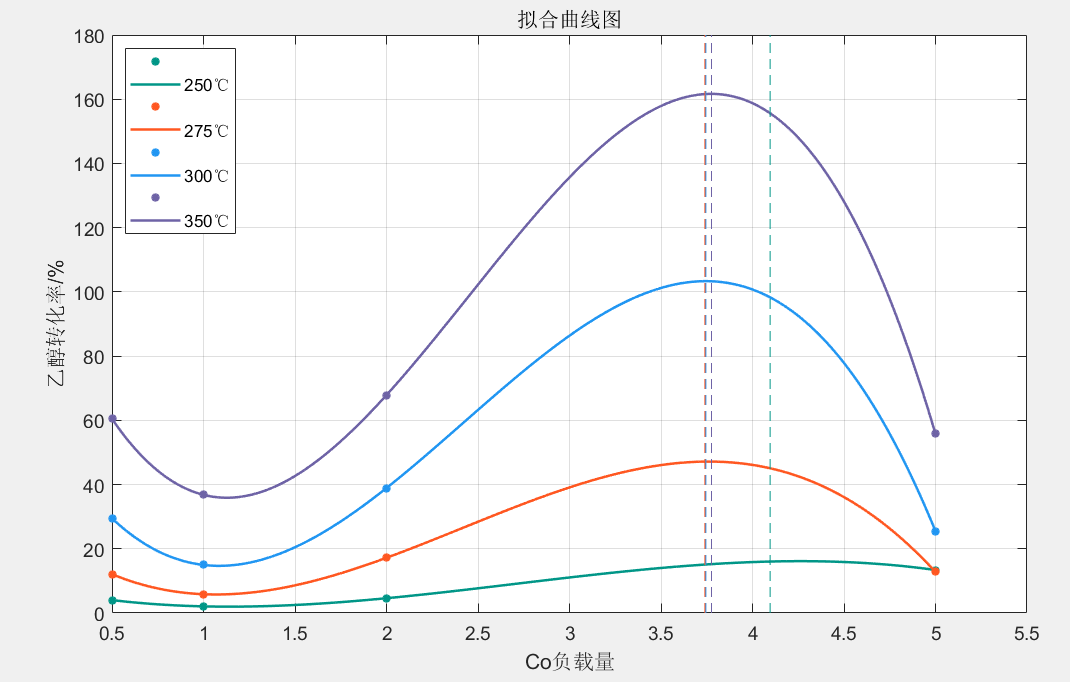
\includegraphics[width=1.0\textwidth]{2_10}
	\caption{乙醇的转化率 -- Co负载拟合曲线}
	\label{fig:circuit-diagram1}
\end{figure}
拟合函数中待估计参数为:
\begin{table}[!htbp]
	\caption{乙醇转化率与Co负载待估计参数}\label{tab:001} \centering
	\begin{tabular}{ccccc}
		\toprule[1.5pt]
		温度(°C) & $p_1$ & $p_2$ & $p_3$  & $p_4$ \\
		\midrule[1pt]
		250 &  -0.9323 &  7.557 & -13.61 &9.051 \\
		275 & -4.243&  30.74 & -51.18 &  30.53\\
		300 &-9.427 &  68.31&  -115 &71.07 \\
		350 &-13.57 &  99.76 & -173.2 & 123.8  \\
		400(Guass) & a=40.03  &   b= 1.353 & c=1.128 & - \\
		\bottomrule[1.5pt]
	\end{tabular}
\end{table}
\newpage
根据图表(图17)分析可得:
\begin{itemize}
	\item 数据走势相对比较曲折,总体可以看作先增加后减少的趋势,为了方便图像描述,采用多项式的拟合方式。
	\item 根据图像显示,Co负载在1左右时可能不能对反应起作用,反而会在一定程度上抑制反应的进行。
	\item 函数图像右侧的极值点对应的横坐标集中在3.75-4.2区间内,分布较为集中,可以为乙醇转化率的最优解提供区间参考。
\end{itemize}


\textbf{乙醇的转化率 -- 乙醇浓度}

实验组A7,A8,A9,A12是关于乙醇浓度的对照组,我们通过函数$f(x) = a*exp(b*x)+c$来拟合乙醇的转化率与乙醇浓度的关系,拟合结果如下:
\begin{figure}[!h]
	\centering
	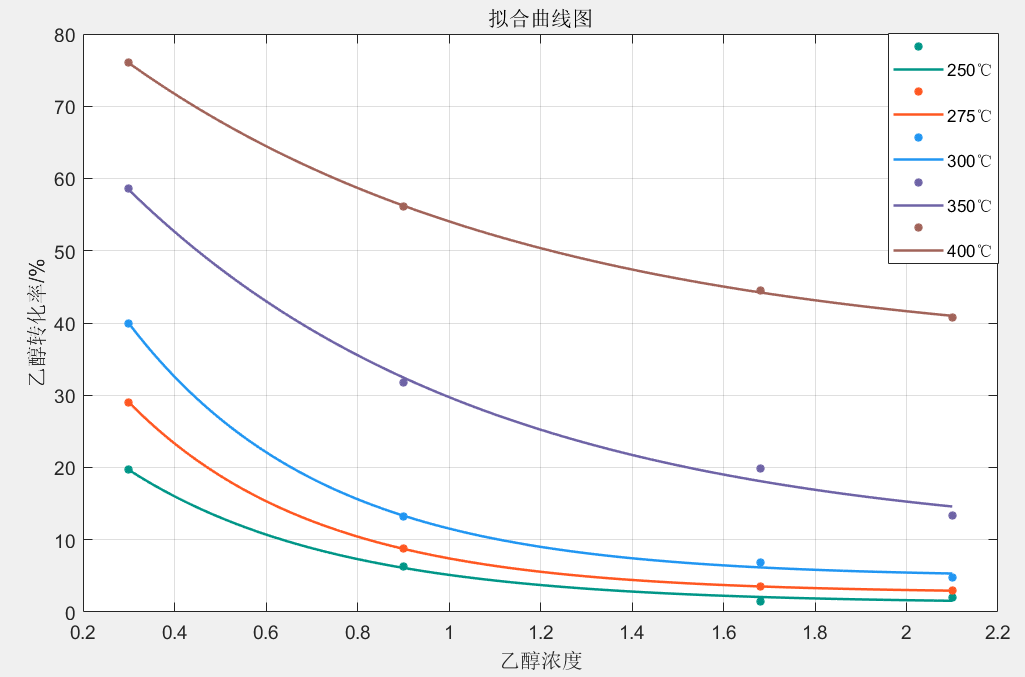
\includegraphics[width=1.0\textwidth]{2_11}
	\caption{乙醇的转化率 -- 乙醇浓度拟合曲线}
	\label{fig:circuit-diagram1}
\end{figure}

根据图表(图18,表7)分析可得:
\begin{itemize}
	\item 数据总体走势呈下降趋势,考虑到随着乙醇浓度的提高,反应速度越来越跟不上乙醇加入的速率,因此乙醇转化率在不断下降,又由于稀释作用,转化率下降的速率将会不断减慢,因此这里采用指数函数进行拟合。
	\item 仍然不排除2.1ml/min后乙醇转化率提高的可能,需要更多的实验数据用于验证。
\end{itemize}

\begin{table}[!htbp]
	\caption{乙醇转化率与乙醇浓度待估计参数}\label{tab:001} \centering
	\begin{tabular}{cccc}
		\toprule[1.5pt]
		温度(°C) & a & b & c \\
		\midrule[1pt]
		250 & 35.84  (-15.85, 87.54) &  -2.21  (-7.501, 3.082) &  1.204  (-9.629, 12.04) \\
		275 & 54.88  (48.62, 61.14) &   -2.436  (-2.847, -2.025) & 2.621  (1.614, 3.628)  \\
		300 &71.37  (3.27, 139.5) & -2.362  (-5.819, 1.096) &  4.824  (-7.101, 16.75) \\
		350 &71.4  (7.616, 135.2) &  -1.265  (-5.548, 3.019) & 9.588  (-53.03, 72.21)  \\
		400 & 56.5  (46.35, 66.66)  &   -1.118  (-1.992, -0.2443) &  35.6  (22.52, 48.67)  \\
		\bottomrule[1.5pt]
	\end{tabular}
\end{table}







\newpage
\textbf{乙醇的转化率 -- Co/SiO2 质量与HAP 质量之和}

实验B1,B2,B3,B4,B6是关于Co/SiO2 质量与HAP 质量和的对照组,我们采用高斯曲线$f(x) =  a*exp(-((x-b)/c)^2)$进行拟合,结果如下:
\begin{figure}[!h]
	\centering
	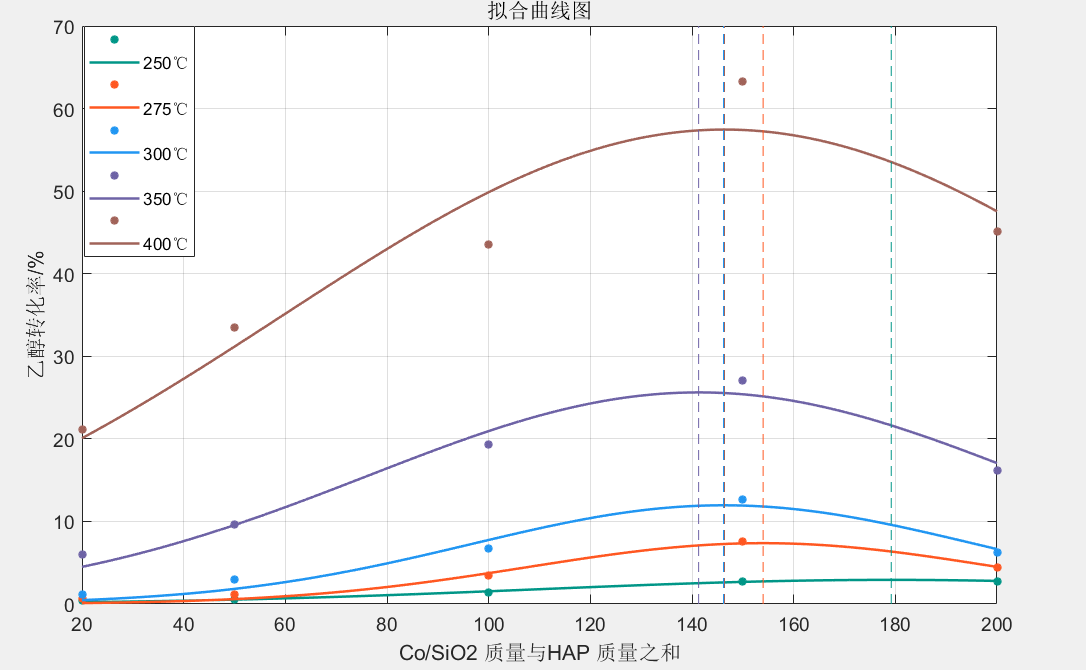
\includegraphics[width=1.0\textwidth]{2_12}
	\caption{乙醇的转化率 -- Co/SiO2 质量与HAP 质量之和}
	\label{fig:circuit-diagram1}
\end{figure}


由图表(图19,表8)分析可知:
\begin{itemize}
	\item 除了Co/SiO2 和 HAP 装料比这个影响因素,观察到数据中存在大量装料比相同而Co/SiO2 质量与HAP 质量之和不同的情况,考虑到催化剂的使用数量也是影响反应的重要因素之一,这里也分析在装料比相同而催化剂的使用数量不同的条件下,对结果产生的影响。
	\item 数据走势为先增加后减小,这里同样采用高斯函数进行拟合,可以得到较好的结果。
	\item 拟合曲线存在最高点,除去偏差较大的250℃曲线,各个曲线取得最高点的横坐标集中在140mg-155mg区间内,分布较为集中,可以为最优解提供区间参考。
\end{itemize}

\begin{table}[!htbp]
	\caption{乙醇的转化率与Co/SiO2 质量与HAP 质量之和待估计参数}\label{tab:001} \centering
	\begin{tabular}{cccc}
		\toprule[1.5pt]
		温度(°C) & a & b & c \\
		\midrule[1pt]
		250 & 2.921  (2.336, 3.506) &  179.2  (142.5, 215.9) &  98.91  (52.35, 145.5) \\
		275 & 7.367  (4.96, 9.774) &  154  (135.9, 172.1)& 65.51  (38.19, 92.83) \\
		300 & 7.367  (4.96, 9.774) & 154  (135.9, 172.1)& 65.51  (38.19, 92.83) \\
		350 &25.62  (18.23, 33.02) &  141.3  (117.3, 165.4)& 91.99  (54.72, 129.3)  \\
		400 &57.46  (35.89, 79.02) &   146.4  (90.98, 201.8)&   123.3  (29.96, 216.5)  \\
		\bottomrule[1.5pt]
	\end{tabular}
\end{table}


\subsubsection{C4烯烃选择性与催化剂组合关系}
\textbf{C4烯烃选择性 -- Co/SiO2和HAP装料比}

A12、A13、A14是关于 Co/SiO2和HAP装料比的对照实验,通过高斯曲线$f(x) =  a*exp(-((x-b)/c)^2)$对C4烯烃选择性与Co/SiO2和HAP装料比的关系进行拟合,拟合图像(图20)如下:

\begin{figure}[!h]
	\centering
	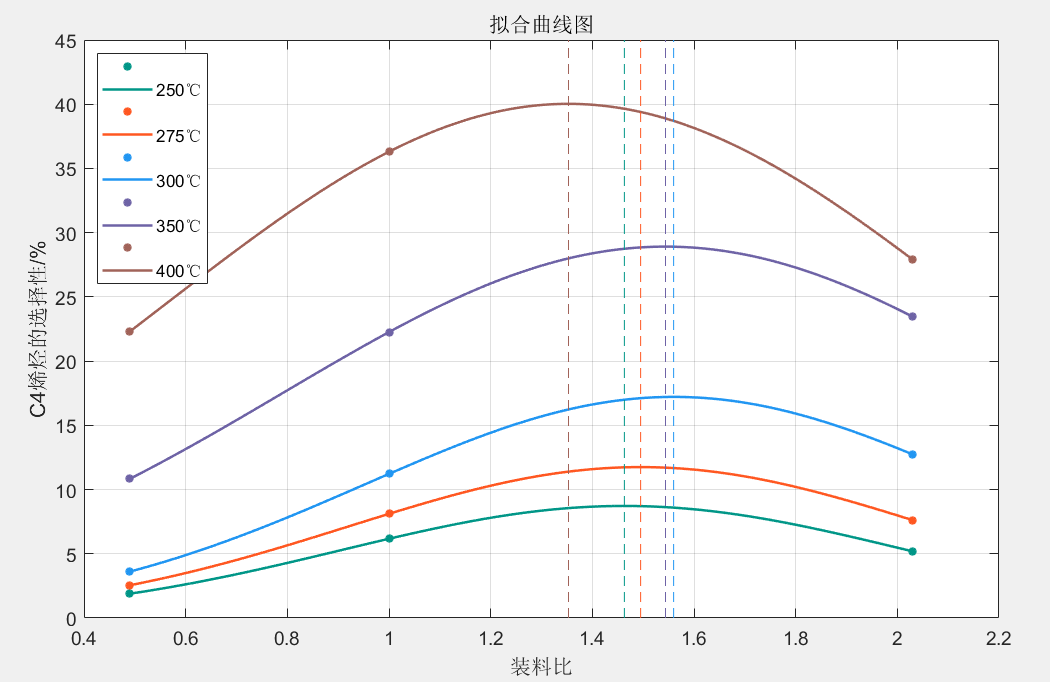
\includegraphics[width=1.0\textwidth]{2_13}
	\caption{C4烯烃选择性 -- Co/SiO2和HAP装料比拟合曲线}
	\label{fig:circuit-diagram1}
\end{figure}

\begin{table}[!htbp]
	\caption{C4烯烃选择性与装料比待估计参数}\label{tab:001} \centering
	\begin{tabular}{cccc}
		\toprule[1.5pt]
		温度(°C) & a & b & c \\
		\midrule[1pt]
		250 & 8.724 &  1.463 &  0.7868 \\
		275 & 11.75 &   1.495 & 0.8131 \\
		300 &17.21 & 1.56&  0.8563 \\
		350 &28.91 &  1.544& 1.063   \\
		400 &40.03 &   1.353 & 1.128 \\
		\bottomrule[1.5pt]
	\end{tabular}
\end{table}
\newpage
由图表(图20,表9)分析可知:
\begin{itemize}
	\item 数据走势为先增加后减小,这里同样采用高斯函数进行拟合,可以得到较好的结果。
	\item 拟合曲线存在最高点,各个曲线取得最高点的横坐标集中在1.3-1.6区间内,分布较为集中,可以为C4烯烃的选择性的最优解提供区间参考。
	\item 图像走势原因同上文对于Co/SiO2 与 HAP 装料比和乙醇转化率的分析。
\end{itemize}


\textbf{C4烯烃选择性 -- Co负载}

实验组A1,A2,A4,A6是与Co负载相关的对照组实验,我们采用线性多项式函数 $f(x) =  a*exp(-((x-b)/c)^2)$对C4烯烃选择性和Co负载的关系进行拟合,
根据图表(图21,表10)分析可知:
\begin{itemize}
	\item C4烯烃的选择性与Co负载非常符合先增后减的趋势,即较为优秀地满足高斯函数的适用拟合特点,也体现出了实际化学原理。
	\item 数据走势一致,有集中的极值点,可以为C4烯烃的选择性的最优解提供区间参考。
	\item 数据走势一致,有集中的极值点,可以为C4烯烃的选择性的最优解提供区间参考。
	3. 300℃的曲线极值远大于其他温度,可以认为在此条件下C4烯烃的选择性的最优解在275℃-350℃附近。
\end{itemize}

\begin{figure}[!h]
	\centering
	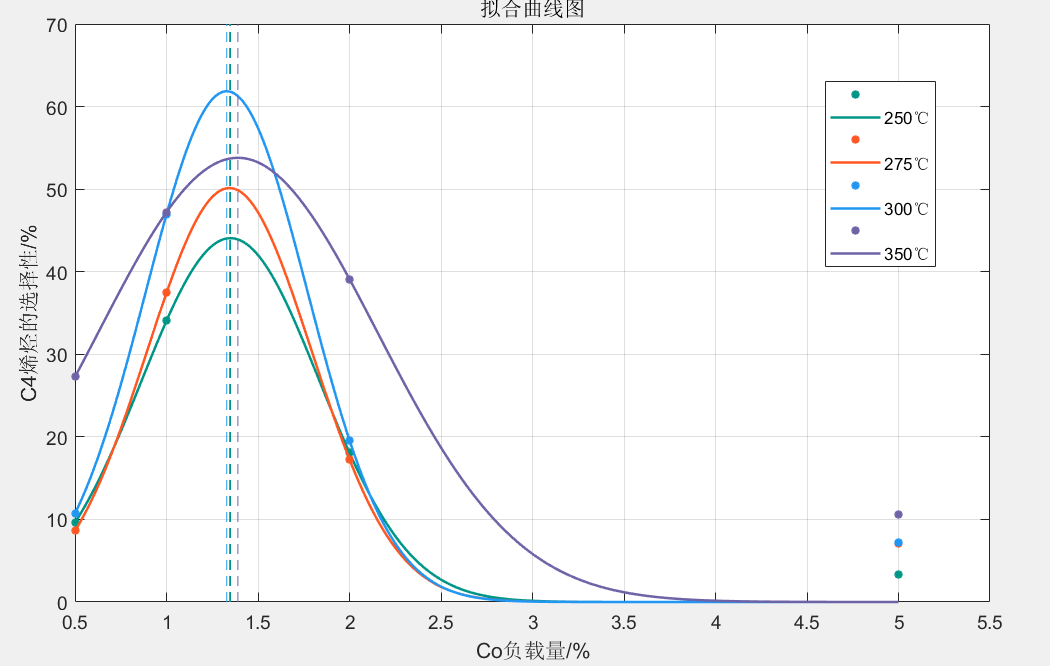
\includegraphics[width=1.0\textwidth]{2_14}
	\caption{C4烯烃选择性 -- Co负载拟合曲线}
	\label{fig:circuit-diagram1}
\end{figure}

\begin{table}[!htbp]
	\caption{C4烯烃选择性与Co负载待估计参数}\label{tab:001} \centering
	\begin{tabular}{cccc}
		\toprule[1.5pt]
		温度(°C) & a & b & c \\
		\midrule[1pt]
		250 & 44.06  (-41.94, 130.1) &  1.35  (0.734, 1.965) &  0.6888  (-0.3731, 1.751) \\
		275 & 50.13  (-162.9, 263.1) &   1.344  (0.1153, 2.572)& 0.6359  (-1.314, 2.586) \\
		300 & 61.85  (-149.4, 273.1) & 1.329  (0.285, 2.373)& 0.6261  (-0.8941, 2.146) \\
		350 &53.79  (-138.7, 246.3) &  1.39  (-0.745, 3.526)& 1.08  (-4.618, 6.778)  \\
		\bottomrule[1.5pt]
	\end{tabular}
\end{table}




\newpage
\textbf{C4烯烃选择性 -- 乙醇浓度}

实验组A7,A8,A9,A12是关于乙醇浓度的对照组,我们通过函数$ f(x) = p_1*x^3 + p_2*x^2 + p_3*x + p_4$来拟合C4烯烃选择性与乙醇浓度的关系,拟合结果如下(图22,表11),分析可知:
\begin{itemize}
	\item 由于乙醇浓度和C4烯烃的选择性相关性不强,这里虽然为了方便展示趋势采用了多项式拟合的方式,但是并不能说明二者存在线性或单调一致关系。
	\item 数据形式可以解释成围绕某个位置的上下浮动。
\end{itemize}

\begin{figure}[!h]
	\centering
	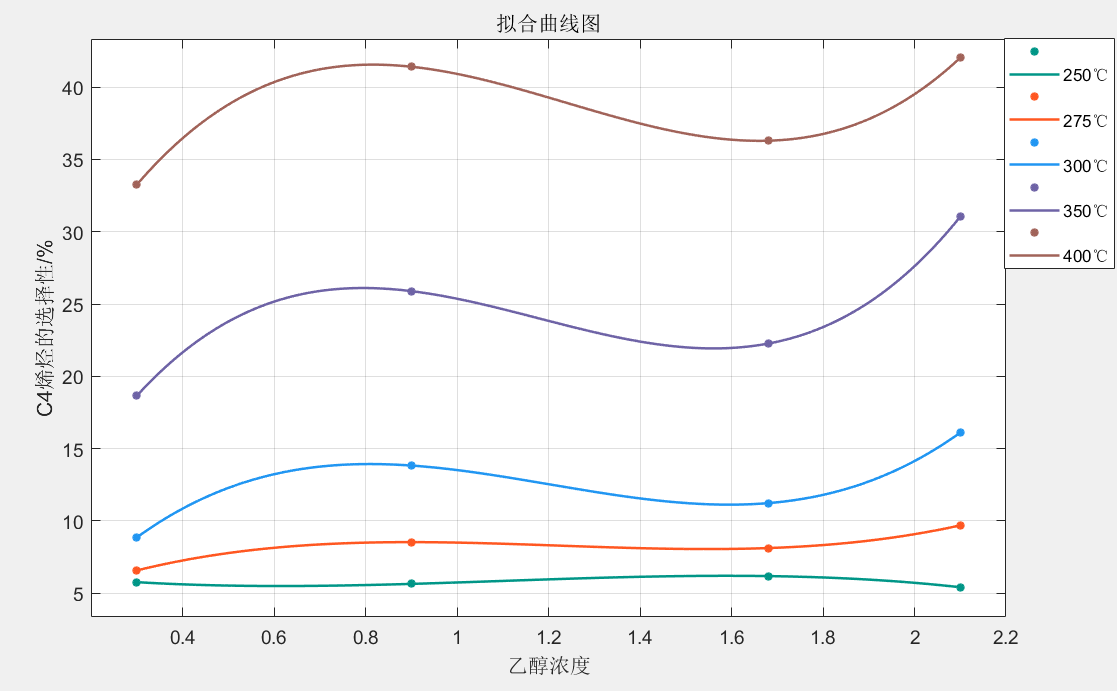
\includegraphics[width=1.0\textwidth]{2_15}
	\caption{C4烯烃选择性 -- 乙醇浓度拟合曲线}
	\label{fig:circuit-diagram1}
\end{figure}
\begin{table}[!htbp]
	\caption{C4烯烃选择性与乙醇浓度待估计参数}\label{tab:001} \centering
	\begin{tabular}{ccccc}
		\toprule[1.5pt]
		温度(°C) & $p_1$ & $p_2$ & $p_3$  & $p_4$ \\
		\midrule[1pt]
		250 &  -1.529 &   5.049 &   -4.47 &6.678  \\
		275 & 3.501&   -12.83 & 14.57 &  3.25 \\
		300 &11.61 &  -41.85&  44.95 &-1.19  \\
		350 &18.57 &  -65.61 &  69.09&  3.317  \\
		400 &  17.49 &   -65 &  71.15 &17.28 \\
		\bottomrule[1.5pt]
	\end{tabular}
\end{table}




\newpage
\textbf{C4烯烃选择性 -- Co/SiO2 质量与HAP 质量之和}

实验B1,B2,B3,B4,B6是关于Co/SiO2 质量与HAP 质量和的对照组,我们采用高多项式$f(x) = p_1*x^4 + p_2*x^3 + p_3*x^2 + p_4*x + p_5$进行拟合,结果如下(图23,表12),分析可知:
\begin{itemize}
	\item 由于Co/SiO2 质量与HAP 质量之和和C4烯烃的选择性相关性不强,这里虽然为了方便展示趋势采用了多项式拟合的方式,但是并不能说明二者存在线性或单调一致关系。
	\item 数据形式可以解释成围绕某个位置的上下浮动。
\end{itemize}
\begin{figure}[!h]
	\centering
	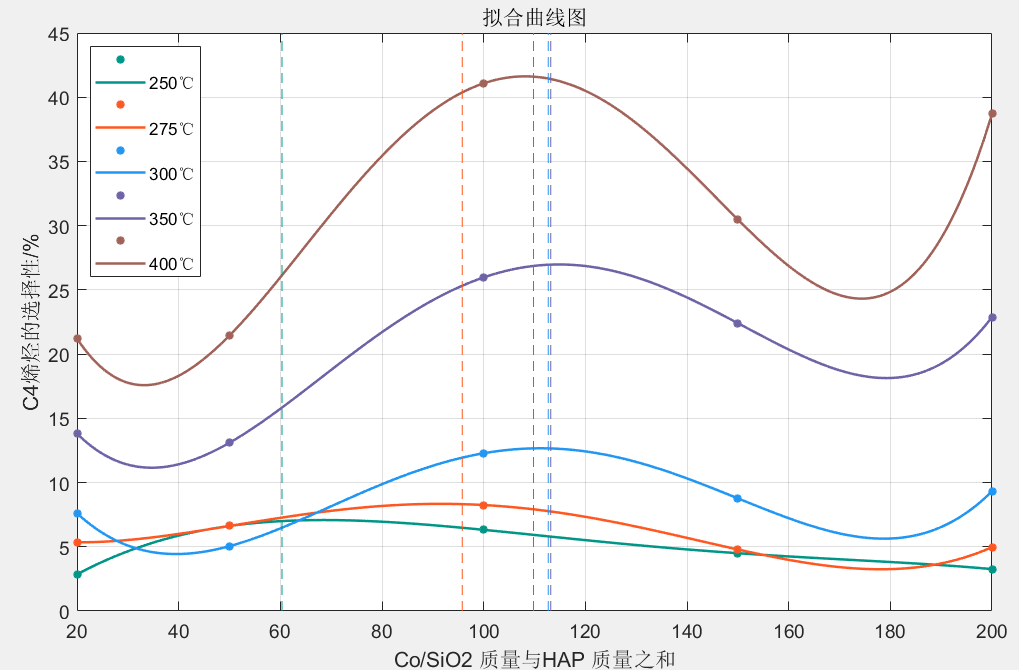
\includegraphics[width=1.0\textwidth]{2_16}
	\caption{C4烯烃选择性 -- Co/SiO2 质量与HAP 质量之和}
	\label{fig:circuit-diagram1}
\end{figure}

\begin{table}[!htbp]
	\caption{C4烯烃选择性与Co/SiO2 质量与HAP 质量之和待估计参数}\label{tab:001} \centering
	\begin{tabular}{cccccc}
		\toprule[1.5pt]
		温度(°C) & $p_1$ & $p_2$ & $p_3$  & $p_4$ & $p_5$ \\
		\midrule[1pt]
		250 & -4.179e-08 &  2.369e-05 & -0.0048 & 0.3778 & -2.968  \\
		275 & 1.03e-07 & -3.985e-05 & 0.0045&  -0.1382 &6.616 \\
		300 & 3.243e-07 &  -0.0001424 &   0.0203 & -1.017 & 20.92 \\
		350 &4.421e-07 &  -0.0001938 & 0.02722& -1.263 &  29.66 \\
		400 & 8.272e-07  &   -0.0003482 & 0.04671 &  -2.072 &  46.61 \\
		\bottomrule[1.5pt]
	\end{tabular}
\end{table}





\subsubsection{C4烯烃收率与催化剂组合关系}
\textbf{C4烯烃收率与Co/SiO2 和 HAP 装料比}

通过观察实验数据发现,A12,A13,A14三组实验关于Co/SiO2 和 HAP装料比互为对照组,我们将基于此拟合C4烯烃收率与Co/SiO2 和HAP装料比之间的函数关系式。通过拟合我们得到如下曲线图:

\begin{figure}[!h]
	\centering
	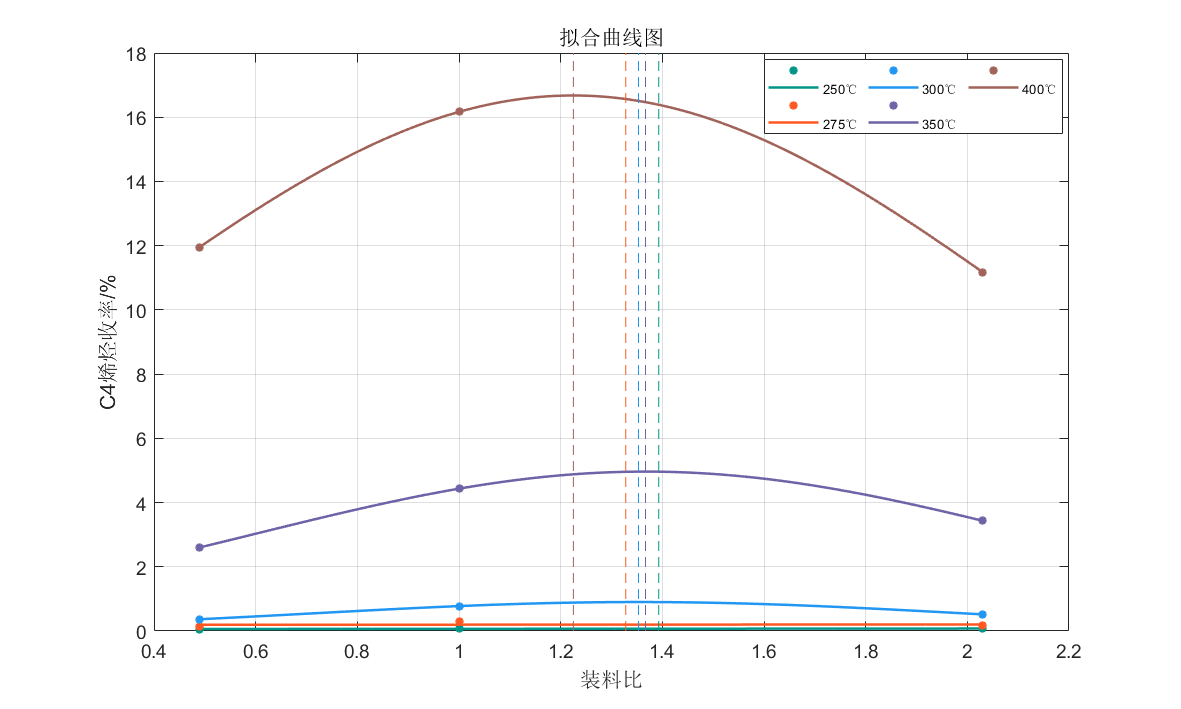
\includegraphics[width=1.0\textwidth]{2_5}
	\caption{C4烯烃收率与装料比拟合曲线}
	\label{fig:circuit-diagram1}
\end{figure}
图中拟合曲线函数式是$f(x) =  a*exp(-((x-b)/c)^2)$,得到的待估计系数分别为:
\begin{table}[!htbp]
	\caption{C4烯烃收率与装料比待估计参数}\label{tab:001} \centering
	\begin{tabular}{cccc}
		\toprule[1.5pt]
		温度(°C) & a & b & c \\
		\midrule[1pt]
		250 & 10.32 &  1.393 &  1.02\\
		275 & 32.13 &  1.328 & 0.9037 \\
		300 &90.19 &1.353&  0.9093 \\
		350 & 496.4 & 1.367& 1.092 \\
		400 & 1668  &  1.225 & 1.273\\
		\bottomrule[1.5pt]
	\end{tabular}
\end{table}

根据拟合情况,我们可以得到以下结论:
\begin{itemize}
	\item 在其他变量一定的情况下,C4烯烃收率与装载比呈现非线性关系。由于数据量较少,对于是否符合高斯曲线不能确定,但基本可以得出:当装载比较低时,C4烯烃收率会随其增大而增大;当过了一定值后,会随其减小而减小。在拟合曲线中大致可以得到装载比的最优解介于1-1.6之间。
	\item 在相同装载比下,当温度介于250-400°C之间时,C4烯烃收率随温度的升高而增大。
	\item 当温度低于350°C时,C4烯烃收率的波动不大,当温度大于350°C,C4烯烃收率波动剧烈。这说明该温度区域内存在特殊温度值使反应变化较大。
\end{itemize}


\textbf{C4烯烃收率与Co负载量关系}

通过观察实验数据发现,A1,A2,A4,A6是关于Co负载量的对照组,我们对其进行高斯曲线拟合,得到拟合图如下:
\begin{figure}[!h]
	\centering
	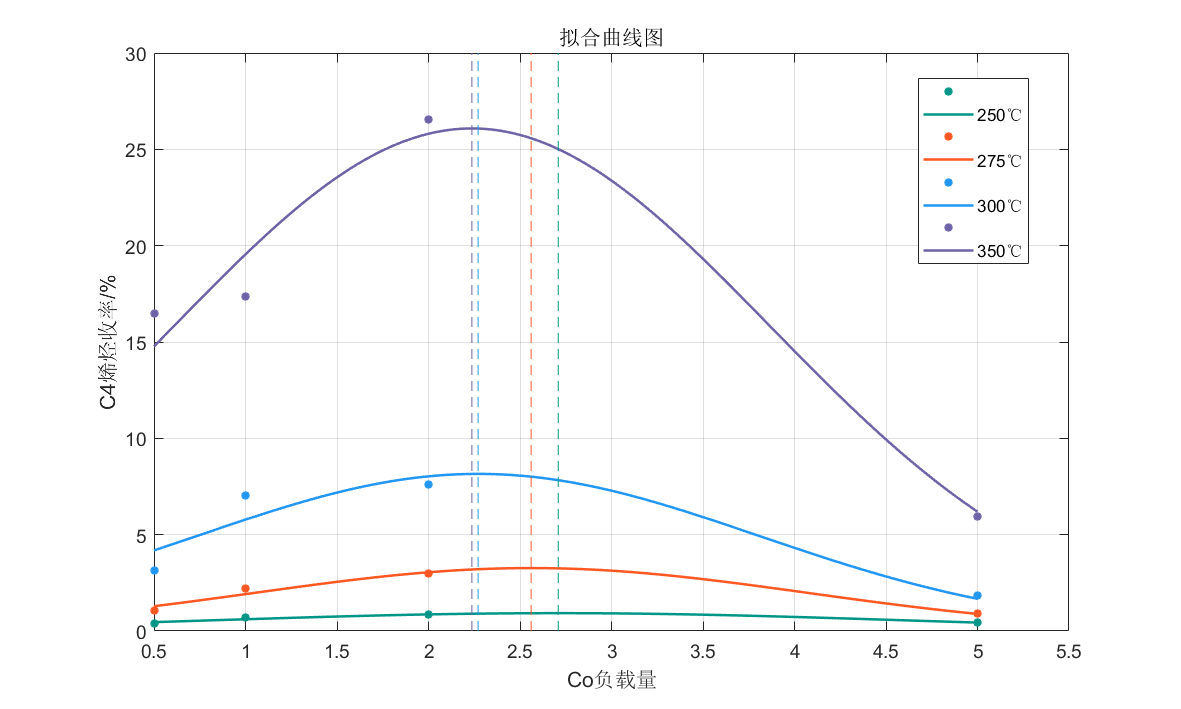
\includegraphics[width=1.0\textwidth]{2_6}
	\caption{C4烯烃收率与Co负载量拟合曲线}
	\label{fig:circuit-diagram1}
\end{figure}
\begin{table}[!htbp]
	\caption{C4烯烃收率与Co负载量待估计参数(置信度95\%)}\label{tab:001} \centering
	\begin{tabular}{cccc}
		\toprule[1.5pt]
		温度(°C) & a & b & c \\
		\midrule[1pt]
		250 &  92.56  (-115.4, 300.5) &  2.709  (-0.772, 6.19) &  2.644  (-3.571, 8.859) \\
		275 & 326.6  (-313.5, 966.8) &   2.561  (-0.4101, 5.532) &2.135  (-1.369, 5.638) \\
		300 &815.4  (-1556, 3187) &2.271  (-3.486, 8.028) &   2.167  (-4.541, 8.875) \\
		350 &  2608  (-1357, 6574) & 2.237  (-0.9082, 5.383) & 2.304  (-1.626, 6.234) \\
		\bottomrule[1.5pt]
	\end{tabular}
\end{table}

图25中拟合曲线函数式是$f(x) =  a*exp(-((x-b)/c)^2)$,得到的待估计系数为表14,分析图像与系数表可知:
\begin{itemize}
	\item 在其他条件不变的情况下,C4烯烃收率与Co负载量呈现高斯曲线关系,且温度越大,该关系越显著。在拟合关系中,可以大致确定当负载量介于1.5-3.5之间时,C4烯烃收率具有最大值,最大值在一定温度范围内,随着温度的升高而升高。
	\item 当Co负载量一定时,C4烯烃收率随温度的升高而增大,且当温度大于300°C时,变化较大。
\end{itemize}


\textbf{C4烯烃收率与乙醇浓度关系}

通过观察实验数据发现,A7,A8,A9,A12是关于乙醇浓度的对照组,我们对其进行高斯曲线拟合,得到拟合图26如下:
\begin{figure}[!h]
	\centering
	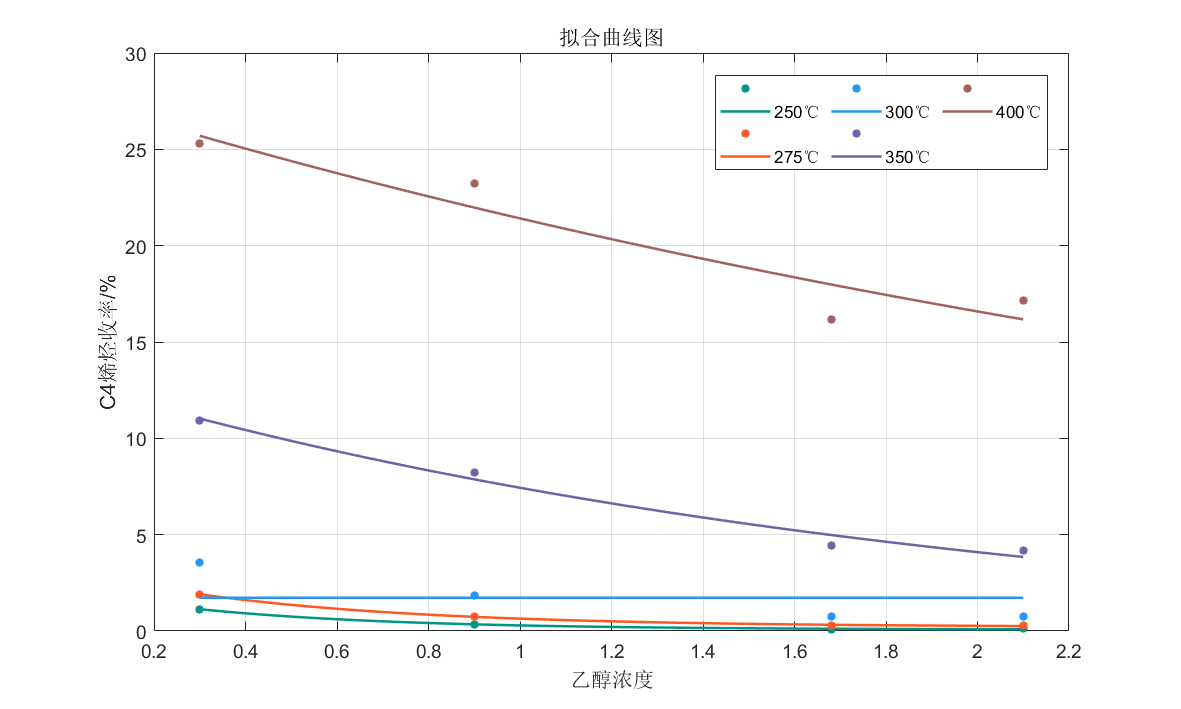
\includegraphics[width=0.8\textwidth]{2_7}
	\caption{C4烯烃收率与乙醇浓度拟合曲线}
	\label{fig:circuit-diagram1}
\end{figure}
\begin{table}[!htbp]
	\caption{C4烯烃收率与乙醇浓度待估计参数值}\label{tab:001} \centering
	\begin{tabular}{cccc}
		\toprule[1.5pt]
		温度(°C) & a & b & c \\
		\midrule[1pt]
		250 &  2.08  (-0.3019, 4.463) &  -2.243  (-6.431, 1.946) &  2.644  (-3.571, 8.859) \\
		275 & 3.052  (0.3372, 5.766) &   -1.953  (-5.329, 1.422) &0.2086  (-0.5851, 1.002) \\
		300 &0.9898 & -168.2 &   1.723  (-18.59, 22.04) \\
		350 &  13.92  (-79.36, 107.2) & -0.5111  (-7.682, 6.66) & -0.9162  (-109, 107.2) \\
		400 &   26.08  (-1123, 1175) & -0.2816  (-18.29, 17.73) &  1.733  (-1196, 1199)  \\
		\bottomrule[1.5pt]
	\end{tabular}
\end{table}

图26中拟合曲线函数式是$f(x) = a*exp(b*x)+c$,得到的待估计系数(表15),分析可知:
\begin{itemize}
	\item 在其他条件不变的情况下,C4烯烃收率随乙醇浓度的升高而降低。乙醇浓度一定时,C4烯烃收率随温度的升高而增大,在介于350-400°C之间变化率较大。
	\item 分析上条性质的具体原因:由附录可知,C4烯烃收率=乙醇转化率$\times$C4烯烃选择性,而乙醇转化率表示单位时间内乙醇的单程转化率,即乙醇转化率=100\% $\times$(乙醇进气量-乙醇剩余量)/乙醇进气量 = 1 - 乙醇剩余量/乙醇进气量。同时,乙醇浓度是指每分钟加入乙醇的量(ml)。因此,当乙醇浓度增大时,乙醇剩余量增大,导致乙醇转化率下降,进一步使C4烯烃收率也跟着下降。
	\item 由于实验数据较少,目前不能得出乙醇转化率的最小值。
\end{itemize}



\textbf{C4烯烃收率与Co/SiO2与HAP 质量之和关系}

通过观察实验数据发现,B1,B2,B3,B4,B6是关于乙醇浓度的对照组,我们对其进行高斯曲线拟合,得到拟合图如下:

\begin{figure}[!h]
	\centering
	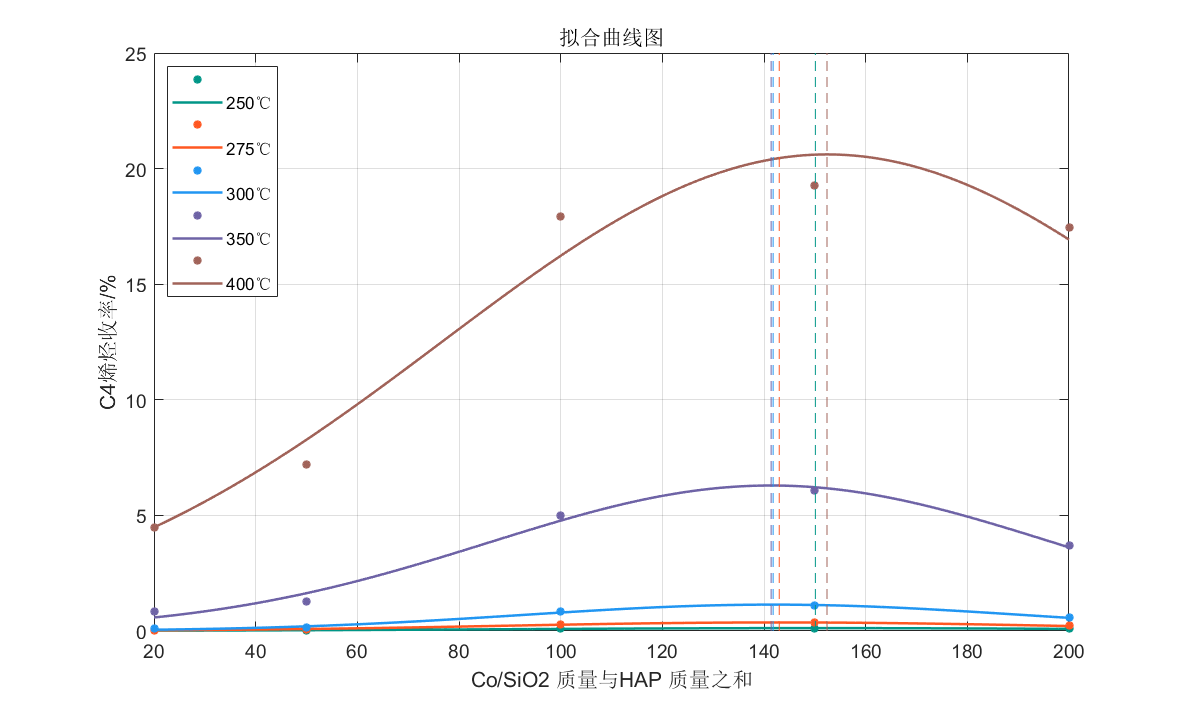
\includegraphics[width=1.0\textwidth]{2_8}
	\caption{C4烯烃收率与Co/SiO2与HAP质量之和拟合曲线}
	\label{fig:circuit-diagram1}
\end{figure}
图27中拟合曲线函数式是$f(x) = a*exp(-((x-b)/c)^2)$,得到的待估计系数(表16).结合图表分析有:
\begin{itemize}
	\item 在其他条件不变的情况下,C4烯烃收率随Co/SiO2与HAP 质量和呈现出先增加后减少的趋势,走势类似于高斯分布,并且C4烯烃收率随温度的上升呈现出加速增加趋势。
	\item 讨论分析走势原因:由可逆反应化学知识得知,Co/SiO2与HAP同作为反应催化剂,在供量较少的情况下并不能进行很好的催化作用,而过量的催化剂有可能影响反应物的浓度,也可能造成其他副产物的增加,因此呈现出先增加后减少的走势。
\end{itemize}   
\begin{table}[!htbp]
	\caption{C4烯烃收率与Co/SiO2与HAP 质量和待估计参数值}\label{tab:001} \centering
	\begin{tabular}{cccc}
		\toprule[1.5pt]
		温度(°C) & a & b & c \\
		\midrule[1pt]
		250 & 0.1244  (0.1154, 0.1334) & 150.1  (144.1, 156.2) &   87.73  (78.46, 96.99) \\
		275 & 0.3702  (0.3178, 0.4227) &   143  (133.7, 152.3) & 77.18  (63.24, 91.13) \\
		300 &1.141  (0.9416, 1.34) & 141.8  (131.7, 151.8) &    69.81  (54.98, 84.64)\\
		350 &  6.293  (4.831, 7.754) & 141.4  (125.9, 156.9) &  78.75  (55.48, 102) \\
		400 &   20.61  (14.69, 26.53) & 152.4  (116.4, 188.5) &  1.733  (-1196, 1199)  \\
		\bottomrule[1.5pt]
	\end{tabular}
\end{table}
 
\newpage    
\subsection{复合因素模型的建立与分析}
为分析催化组合中各因素对乙醇转化率、C4烯烃选择性、C4烯烃收率的共同作用,我们首先分析各因素所占的影响权重。为了刻画这一特性,我们采用SPSS软件中的多层感知机神经网络进行训练,训练后权重结果如下:

\begin{figure}[!h]
	\centering
	\begin{minipage}[c]{0.45\textwidth}
		\centering
		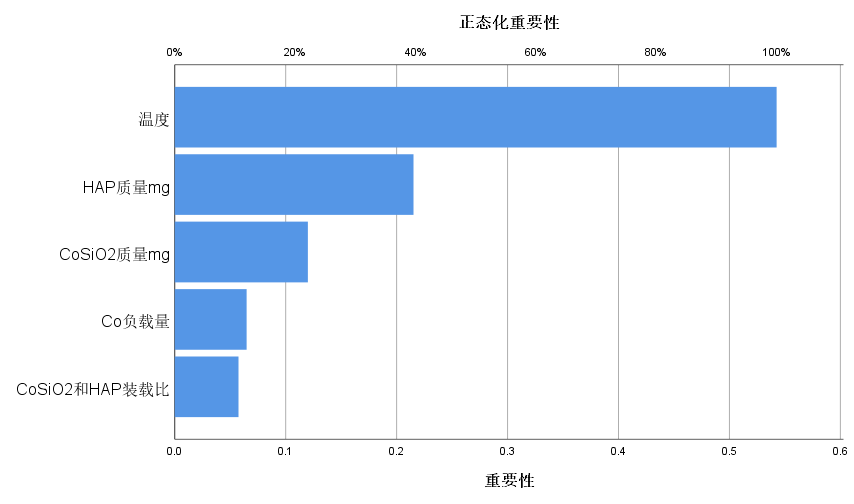
\includegraphics[width=0.95\textwidth]{4_17}
		\subcaption{乙醇转化率影响因素权重分析}
		\label{fig:sample-figure-a}
	\end{minipage}
	\begin{minipage}[c]{0.45\textwidth}
		\centering
		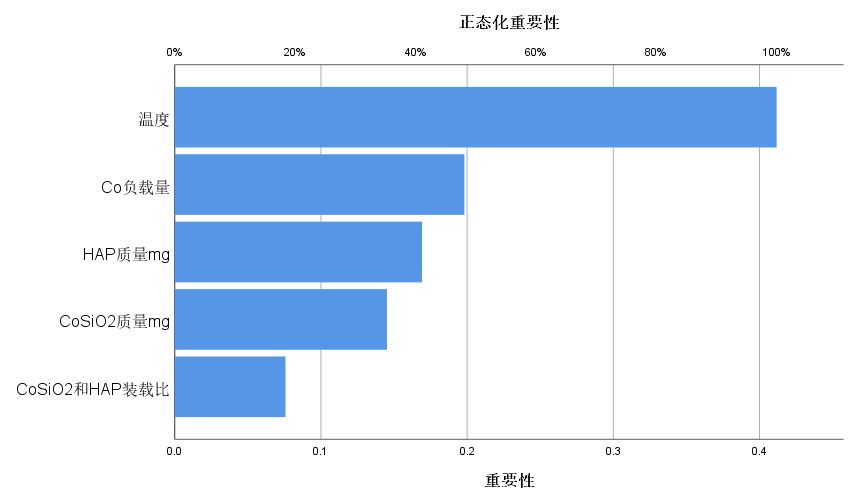
\includegraphics[width=0.95\textwidth]{4_18}
		\subcaption{C4烯烃选择性影响因素权重分析}
		\label{fig:sample-figure-b}
	\end{minipage}
	\caption{权重分析}
	\label{fig:sample-figure}
\end{figure}

\begin{figure}[!h]
	\centering
	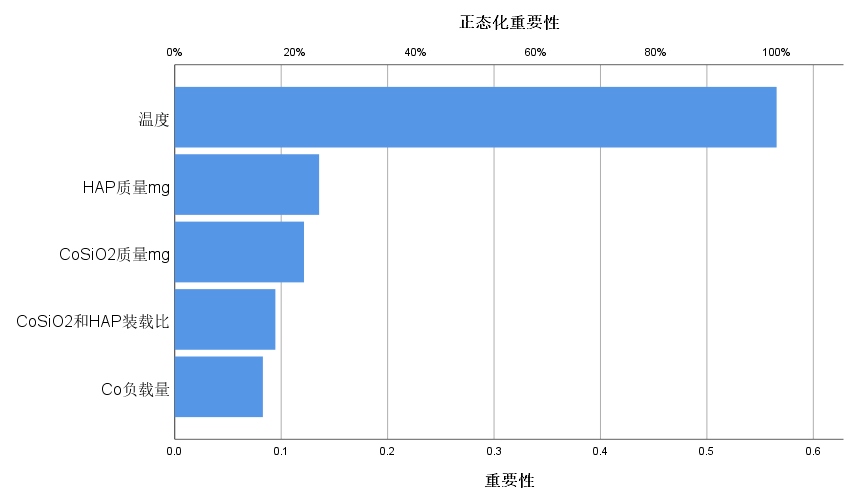
\includegraphics[width=0.7\textwidth]{4_16}
	\caption{C4烯烃收率影响因素权重分析}
	\label{fig:circuit-diagram1}
\end{figure}
综合上述3张权重分析图可知,温度在所有影响因素中权重最大,为100\%,且与权重第二大的影响因素差距较大,是影响三个指标的最关键的因素。至于其它四个影响因素所占权重则相差不大,且都没有超过50\%。图片显示,HAP质量、Co负载量、HAP质量分别是影响乙醇转化率、C4烯烃选择性、C4烯烃收率的次关键的因素。而在五个影响因素中,Co/SiO2和HAP装载比对乙醇转化率和C4烯烃选择性的影响程度最小,Co负载量对C4烯烃收率所产生的影响最小。

然而,权重分析只能粗略地得到乙醇转化率、C4烯烃选择性与催化剂组合和温度的定性关系,我们将在通过Adaboost+决策树+RSM算法流程来详细分析定量关系(详见7.3.3中响应曲面分析)。

     

\newpage
\section{问题三的模型建立与求解}
\subsection{问题的分析}
问题三是典型的优化问题,但所给数据组合的低差异性给最优化带来了困难。我们通过SPSS软件初步为变量之间建立联系函数,但在拟合和预测方面最高时$R^2$的值是0.76左右,因此,我们放弃了传统了解决方案,尝试寻找一些较好的机器学习方法。

在该优化问题中,因变量是C4烯烃收率,我们的目标是使该值尽可能大。自变量包括Co负载量、Co/SiO2和HAP装料比、乙醇浓度以及温度。其中Co/SiO2和HAP装料比是由Co/SiO2的质量和HAP的质量决定的,且在催化剂组合中给出了明确的数值。除此之外,A11组中没有HAP,但与其它组并没有形成对照,因此我们无法通过已有数据分析出有无HAP对C4烯烃收率的具体影响。因此,我们在分析C4烯烃收率与催化剂组合之间的关系时,对数据的预处理主要做了以下两件事:
\begin{itemize}
	\item 将A11组中的数据剔除;
	\item 对于Co/SiO2和HAP装料比,我们可以将其看作两个独立的因变量,即Co/SiO2的质量和HAP的质量。通过这种方式,我们可以将催化剂的具体质量纳入反应体系。
	\item 在实际训练时,Co/SiO2和HAP装料比与Co/SiO2的质量和HAP的质量可以是互斥的,即每次只能出现其中一个,也可以是不互斥的,即两者可以同时出现,这主要取决于具体模型的训练结果。
\end{itemize}

经过多次实验测试后,我们选择AdaBoost回归算法进行组合最优化分析,其中在该算法内部,则使用决策树作为分类器的分类算法。

\subsection{模型的建立}
\subsubsection{Adaboost回归预测模型建立}
Adaboost算法是一种既可以用于分类也可以用于回归分析的迭代算法,其基本思想是针对同一训练集中的不同分类器(弱分类器),将这些弱分类器连接起来,从而构成一个更强的分类器(强分类器)。这样的特征对于我们的数据具有很高的契合度,由于实验所给数据中自变量很多都是大量的重复值,通过简单的一次回归很难得到之间的函数关系,所以在多层分类的基础上,它可以得到各自变量对因变量的影响程度,并深度挖掘其中的深层联系,从而克服重复数据带来的困扰。

对于给定的训练集$D=\left\{\left(x_{i},y_{i}\right)\right\}_{i=1}^{m}$,其中$m$为训练样本数。使用Adaboost算法进行回归大致有以下流程:
% 插入单张图片
\begin{figure}[!h]
	\centering
	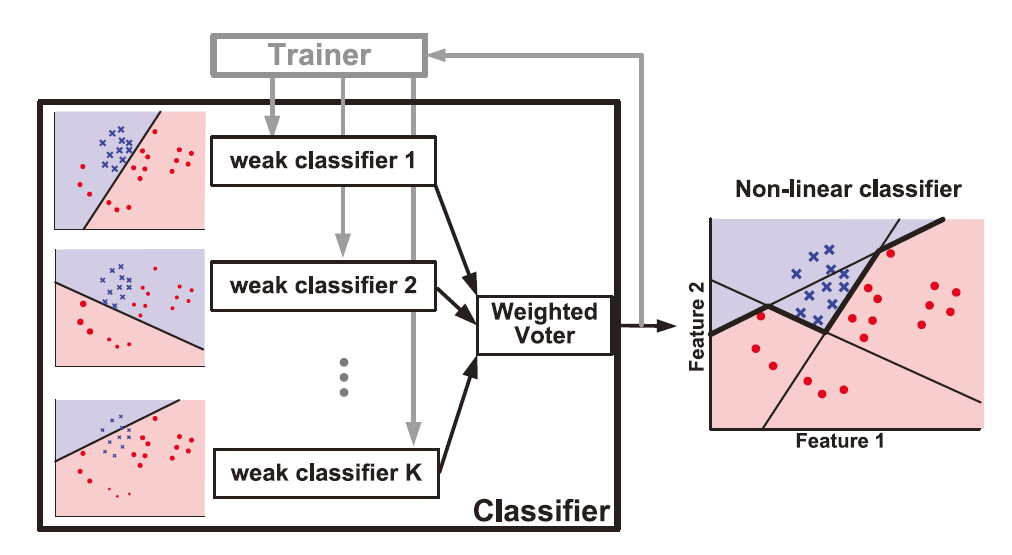
\includegraphics[width=.6\textwidth]{ad}
	\caption{Adaboost回归算法原理图}
	\label{fig:circuit-diagram}
\end{figure}

\begin{enumerate}
	\item 初始化训练样本权重为$\frac{1}{m}$
	\begin{equation*}
		\mathcal{D}_{1}=\left(w_{11}, \ldots, w_{1 i}, \ldots, w_{1 m}\right), w_{1 i}=\frac{1}{m}, i=1,2, \ldots, m
	\end{equation*}
	
	\item 对迭代轮次${t = 1,2,\ldots, T}$,其中$T$为最大的训练循环次数。
	\begin{enumerate}
		\item 使用当前样本分布${\mathcal D}_t$的训练弱分类器(weak classifer)
		\begin{equation*}
		{h_t} = \mathfrak{L}\left( {D,{​{\mathcal D}_t}} \right)
		\end{equation*}		
		\item 计算弱分类器上样本的最大误差:
		\begin{equation*}
		 E _ { t} = \max \left| y _ { i } - h _ { t } \left( x _ { i } \right) \right|, i = 1,2 \ldots m
		 \end{equation*}
		 
		 \item 计算每个样本的相对误差:
		 
		  如果是线性误差,则
		  \begin{equation*}
		  e _ { t i } = \frac { \left| y _ { i } - h_t \left( x _ { i } \right) \right| } { E _ { t } }
		  \end{equation*}
		 
		 如果是平方误差,则
		 \begin{equation*}
		 e _ { t i } = \frac { \left( y _ { i } - h _ { t } \left( x _ { i } \right) \right) ^ { 2 } } { E _ { t } ^ { 2 }}
		\end{equation*}
		 
		 如果是指数误差,则
		 \begin{equation*}
		 e _ { t i } = 1 - \exp \left( \frac { - \left| y _ { i } - h _ {t } \left( x _ { i } \right) \right| } { E _ { t} } \right)
		\end{equation*}
		 
		 \item 弱分类器$h_t$在训练数据集上的回归误差率:
		 \begin{equation*}
		  \varepsilon _ { t } = \sum _ { i = 1 } ^ { m } w _ { t i } e _ { t i }
		 \end{equation*}
		
		 
		 \item 选择弱分类器$h_t$的合适阈值${\alpha _t}$,从而使误差最小:
		 \begin{equation*}
		  {\alpha _t} = \frac{​{​{\varepsilon _t}}}{​{1 - {\varepsilon _t}}}
		 \end{equation*}
		 
		 \item 更新训练集的样本权重${​{\mathcal D}_{t + 1}} = \left( {​{w_{t + 1,1}}, \ldots ,{w_{t + 1,i}}, \ldots ,{w_{t + 1,m}}} \right)$:
		 \begin{equation*}
		 w _ { t + 1 , i } = \frac { w _ { t i } } { Z _ {t } } \alpha _ { t } ^ { 1 - e_ {ti} }
		\end{equation*}
		 其中,${​{Z_t}}$是规范化因子:
		 \begin{equation*}
		 		  Z _ { t } = \sum _ { i = 1 } ^ { m } w _ { t i } \alpha _ { t } ^ { 1 - e_{ti} }
		 \end{equation*}
	
	\end{enumerate}
	\item 经过$T$次循环后,得到$T$个弱分类器,按权重进行线性组合:
	\begin{equation*}
		\sum\limits_t^T {​{\alpha _t}{h_t}\left( x \right)}
	\end{equation*}
	由此得到最终的强分类器(Weighted Voter):
	\begin{equation*}
		H( x ) = \sum _ { t = 1 } ^ { T } \left( \ln \frac { 1 } { \alpha _ { t } } \right) g ( x )
	\end{equation*}
	其中,$g(x)$是所有${\alpha _t}{h_t}\left( x \right),t=1,2,...,T$的中位数。
	\item  输出:强分类器$H(x)$的回归结果。
\end{enumerate}

更进一步,对于分类器中的分类算法,一般有决策树分类器、KNN分类器和多层感知机。经过我们多次实验,在我们的数据集上,决策树分类器具有良好的性能,其主要原因可能是虽然我们的实验数据变量是连续性变量,但所提供的数据中的重复性导致其具有离散化的特征,这比较适合与决策树的逐层分类模型。

\subsubsection{仿真RSM模型求解最优值建立}
响应曲面设计方法(Response Surface Methodology, RSM)是一种利用合理的试验设计方法并通过实验得到一定的数据,采用多元二次回归方程来拟合因素与响应值之间的函数关系,通过对回归方程的分析来寻求最优工艺参数,解决多变量问题的一种常见的回归设计方法。

在RSM方法的启发下,我们在第二问中已经得到每个自变量最优解的上下限,因此可以通过RSM设计一些合理的自变量参数组合(即催化剂组合以及温度的组合方案), 并将RSM生成的实验设计数据作为输入值在上述已训练好的Adaboost回归模型中进行预测,以获得实验结果(C4烯烃收率)。简而言之,我们将传统RSM实验中本应由真实实验获得响应值用机器学习算法进行预测,从而获得预测的实验数据,相当于做了“虚拟实验”,故将其成为"仿真RSM模型"。

为了确保可以使用RSM模型进行求解最优值,其一般需要满足以下条件:
\begin{itemize}
	\item 确信或怀疑因素对指标存在非线性的影响。根据第一问和第二问建立的拟合函数可知,该条件成立。
	\item 因素个数2-7个,一般不超过4个。本实验中需要研究的影响因素只有4个。
	\item 所有因素均为计量值数据。
	\item 实验区域已接近最优区域。根据第二问中通过控制变量法对自变量进行逐一分析,我们可以基本确定取得最优解时自变量的范围。
\end{itemize}

RSM一般采用中心复合实验设计(CCD)或者Box-Behnken实验设计(BBD),这里我们采用的BBD的实验设计方法。

\subsection{模型求解}
\subsubsection{Adaboost回归模型求解}
为了获取C4烯烃收率与催化剂组合和温度之间的回归关系,基于上述模型,我们借助SPSS和MPai数据科学平台进行计算。在SPSS上,我们采用多层感知器神经网络进行预测,经多次调参分析,$R^2$最大仅有0.76。Mpai数据科学平台提供了多种机器学习算法的模型,每个模型具有详细的参数的配置,下面详细介绍使用Adaboost回归模型求解模型。

\begin{table}[!htbp]
	\caption{Adaboost回归模型基本参数表}\label{tab:001} \centering
	\begin{tabular}{cccc}
		\toprule[1.5pt]
		 参数名& 训练占比 & 定量数据是否标准化 & 定类数据独热编码 \\
		\midrule[1pt]
		取值 &  0.00-1.00 & z-score标准化/均值标准化/min-max标准化 & 是/否 \\
		\bottomrule[1.5pt]
	\end{tabular}
\end{table}

\begin{table}[!htbp]
	\caption{Adaboost回归模型高级参数表}\label{tab:001} \centering
	\begin{tabular}{cccccc}
		\toprule[1.5pt]
		参数名& 数据洗牌 & 交叉验证 & 随机种子 & 基础分类器 & 学习率 \\
		\midrule[1pt]
		取值 &  是/否 & 是/否 &   0 $\geq$ & 决策树/KNN/多层感知机 &
		0.0-1.0 \\
		\bottomrule[1.5pt]	
	\end{tabular}
\end{table}

由于数据集较少,我们将训练占比固定为$0.75$,对于一些影响较小的参数,我们采用默认值,即独热编码选项为否,数据洗牌选项为是,交叉验证否,随机种子0。对于剩下的参数配置,经过多次实验,我们得到如下部分实验结果(表20).通过实验发现,M3的参数配置(决策树+0.2学习率)具有较好的性能,其平均绝对误差(MAE)为0.4839,决定系数$R^2$为0.9869,因此该模型的拟合优度较高。于是,我们采用实验数据中的催化剂和温度预测C4烯烃收率,预测部分结果如下(表19):
\begin{table}[!htbp]
	\caption{Adaboost回归模型高级参数表}\label{tab:001} \centering
	\begin{tabular}{cccccc}
		\toprule[1.5pt]
		真实值(\%)& 19.27714862
		& 0.504396302
		& 0.359741111
		& 1.042826728
		& 0.069906624
		\\
		预测值(\%) &  11.95620228
		& 0.518101314
		&   0.281711425
		& 2.190299165
		&
		0.088997091
		\\
		\bottomrule[1.5pt]	
	\end{tabular}
\end{table}


\begin{table}[!htbp]
	\caption{Adaboost回归模型部分实验数据}\label{tab:001} \centering
	\begin{tabular}{cccccccc}
		\toprule[1.5pt]
		组号 & M1 & M2 & M3 & M4 & M5 & M6 & M8 \\
		\midrule[1pt]
		分类器& 决策树 & 决策树 &  决策树 & 决策树 & KNN & KNN & 多层感知机 \\
		标准化&  否 & 均值 &  否 & 否 & 否 & 否 & 否 \\
		学习率 &  1 & 1 &  0.2 & 2 & 1 & 0.2  & 1  \\
		MSE & 3.7967
		 & 11.3034
		  &  2.2609
		   & 18.6175
		    & 11.3758
		    & 12.9248
		      & 104.0716
		         \\
		RMSE &  1.9485
		 & 0.0698
		  &  1.5036
		  & 4.3148
		   & 3.3728
		   & 3.5951
		     & 10.2015
		        \\
		MAE &  1.0427
		 & 0.0484
		  &  0.4839
		   & 1.5151
		    & 2.9437
		     & 2.0025
		       & 7.8231
		          \\
		$R^2$ &  0.9574
		 & 0.8334
		  &  0.9869
		  &0.8918
		   & 0.9339
		    & 0.9267
		      &0.5403
		         \\
		MAPE &  477.7233
		 & 244.7899
		  &  50.9129
		   & 318.6526
		    & 1466.3993
		     & 46.0267
		       &74.9476
		         \\
		\bottomrule[1.5pt]	
	\end{tabular}
\end{table}

上述结果均证明Adaboost+决策树回归模型具有较高的预测精度,这为通过RSM模型求解最优组合提供了可靠的基础。


\subsubsection{仿真RSM模型求解}
根据RSM模型中的BBD法的基本方案,我们将求解过程分为以下几个步骤。

\textbf{1. 确定实验因素}

由第二问的实验分析,C4烯烃收率与温度、Co负载量、Co/SiO2和HAP装料比、乙醇浓度都具有显著的相关性。由于Co/SiO2和HAP装料比是由Co/SiO2的质量和HAP的质量直接影响的,如果将三者同时作为RSM模型中的影响因素,由于需要确定变量的上下限,所以会导致生成实验设计方案中的Co/SiO2和HAP装料比与两者之间质量比不相符。为了避免这个问题,我们将该影响因素转变为Co/SiO2和HAP装料比与Co/SiO2和HAP的质量总和,这样也可以通过总质量和质量比确定Co/SiO2和HAP的实际质量。

\textbf{2. 确定因素的水平范围}

一般可以通过做单因素初步实验(控制变量法)或由样品的特性和工艺来确定BBD设计所研究的因素水平范围。需要注意的是,合适的因素水平范围对获得理想的优化结果非常重要,如果水平范围太窄会得不到优化结果,太宽则会使结果的精度降低。

通过第二问对C4烯烃收率与催化剂组合和温度之间的关系,我们可以得到每一因素的基本水平范围如下:

\begin{table}[!htbp]
	\caption{仿真RSM试验因素水平表}\label{tab:001} \centering
	\begin{tabular}{ccc}
		\toprule[1.5pt]
		因素& 下限 & 上限 \\
		\midrule[1pt]
		温度 &  400.00 & 500.00 \\
		Co负载量 &  2.00 & 3.00 \\
		Co/SiO2和HAP装料比 &  1.00 & 1.60 \\
		乙醇浓度 &  0.20 & 1.60 \\
		Co/SiO2和HAP总质量 &  80.00 &  400.00\\
		\bottomrule[1.5pt]	
	\end{tabular}
\end{table}


\textbf{3.实验设计安排及结果}

根据Box-Behnken中心组合设计原理,在控制变量法的基础上,以温度、Co负载量、Co/SiO2和HAP装料比、乙醇浓度与Co/SiO2和HAP总质量五个因素为自变量,C4烯烃收率为响应值,作五因素三水平的响应面分析实验,共46个试验点。RSM试验的因素与水平组合的试验表详见附件“我的支撑材料-RSM试验表.csv”。部分示例数据如下所示:
\begin{figure}[!h]
	\centering
	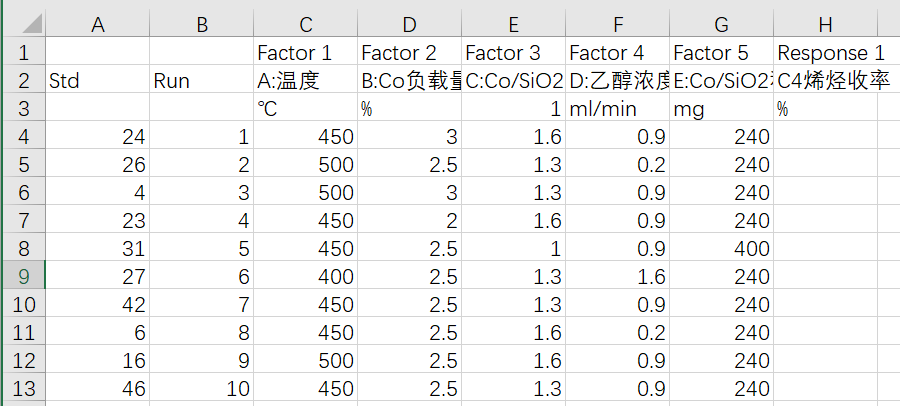
\includegraphics[width=1.0\textwidth]{3_1}
	\caption{RSM试验的因素与水平组合的试验表}
	\label{fig:circuit-diagram1}
\end{figure}

\textbf{4.实验获取数据}

由于RSM中的自变量与Adaboost回归模型中所用的具有一定的转换关系,即可以通过RSM中的Co/SiO2和HAP装料比与Co/SiO2和HAP总质量获得Co/SiO2和HAP的实际质量(mg)。然后根据3中设计的实验组合方案,我们将其在已训练好的Adaboost回归模型上进行预测,代替真实实验数据,从而获得C4烯烃收率的数据。详细数据见附件“我的支撑材料-RSM预测表.xlsx”。部分示例数据如下:
\begin{figure}[!h]
	\centering
	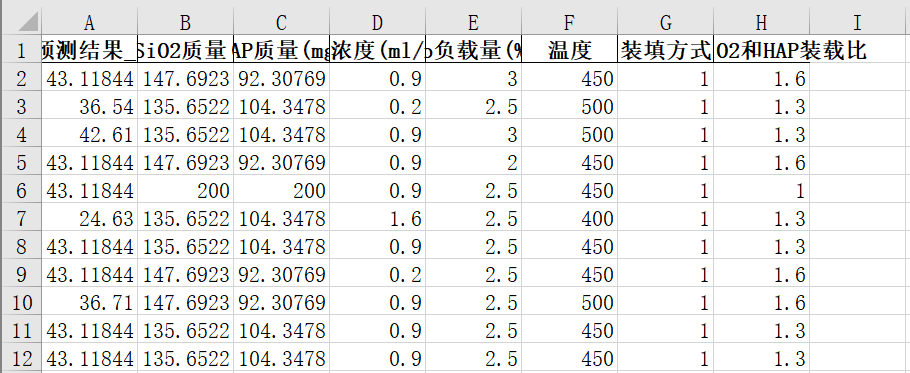
\includegraphics[width=1.0\textwidth]{3_2}
	\caption{RSM响应值预测数据表}
	\label{fig:circuit-diagram1}
\end{figure}

\textbf{5.软件分析}

我们将4中表中的预测数据对应填入3中的响应值C4烯烃收率中,然后借助Design-Expert软件对实验数据统计分析,求解最优的催化剂组合与温度。


\subsubsection{仿真RSM模型结果分析}
\textbf{1.方差分析}

为建立响应性曲面,Design-Expert提供了多种模型,经多次测试,发现四次交叉回归方程具有良好的拟合效果。为证明试验数据的合理性,我们先进行响应曲面四次模型的方差分析,结果如下表(图33).
\begin{figure}[!h]
	\centering
	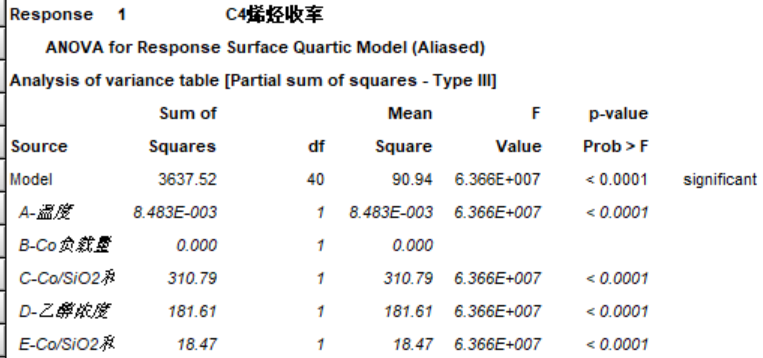
\includegraphics[width=1.0\textwidth]{3_3}
	\caption{响应曲面四次模型的方差分析(部分)}
	\label{fig:circuit-diagram1}
\end{figure}
由表中数据可知,P值均小于$0.0001$,这说明模型具有较强的显著性(significant)。为了方便表示,给每一个因素编号A,B,C,D,E,具体含义见图33.


\textbf{2.四次模型系数}

进一步,我们可以得到响应曲面四次模型中的各因素所对应的系数如下:

$C4\text{烯烃收率}	 =
+43.12
+0.046	 * A
+0.000	 * B
+8.81	 * C
-6.74	 * D
+2.15	 * E
+0.000	 * A * B
+1.47	 * A * C
-1.99	 * A * D
-2.75	 * A * E
+0.000	 * B * C
+0.000	 * B * D
+0.000	 * B * E
-0.11	 * C * D
-8.81	 * C * E
+6.74	 * D * E
-10.05	 * A^2
+6.87	 * B^2
-1.95	 * C^2
-4.46	 * D^2
-6.87	 * E^2
+0.000	 * A^2 * B
-7.35	 * A^2 * C
+2.53	 * A^2 * D
-1.99	 * A^2 * E
+8.01	 * A * B^2
+3.60	 * A * C^2
+1.70	 * A * D^2
-8.81	 * B^2 * C
+0.44	 * B^2 * D
-2.15	 * B^2 * E
+0.000	 * B * C^2
+0.000	 * B * D^2
+0.33	 * C^2 * D
+6.67	 * C^2 * E
-8.93	 * C * D^2
-5.38	 * A^2 * B^2
-0.98	 * A^2 * C^2
-8.742E-003	 * A^2 * D^2
-4.92	 * B^2 * C^2
-8.70	 * B^2 * D^2
$


\bigskip
\textbf{3.预测值与真实值}

\begin{figure}[!h]
	\centering
	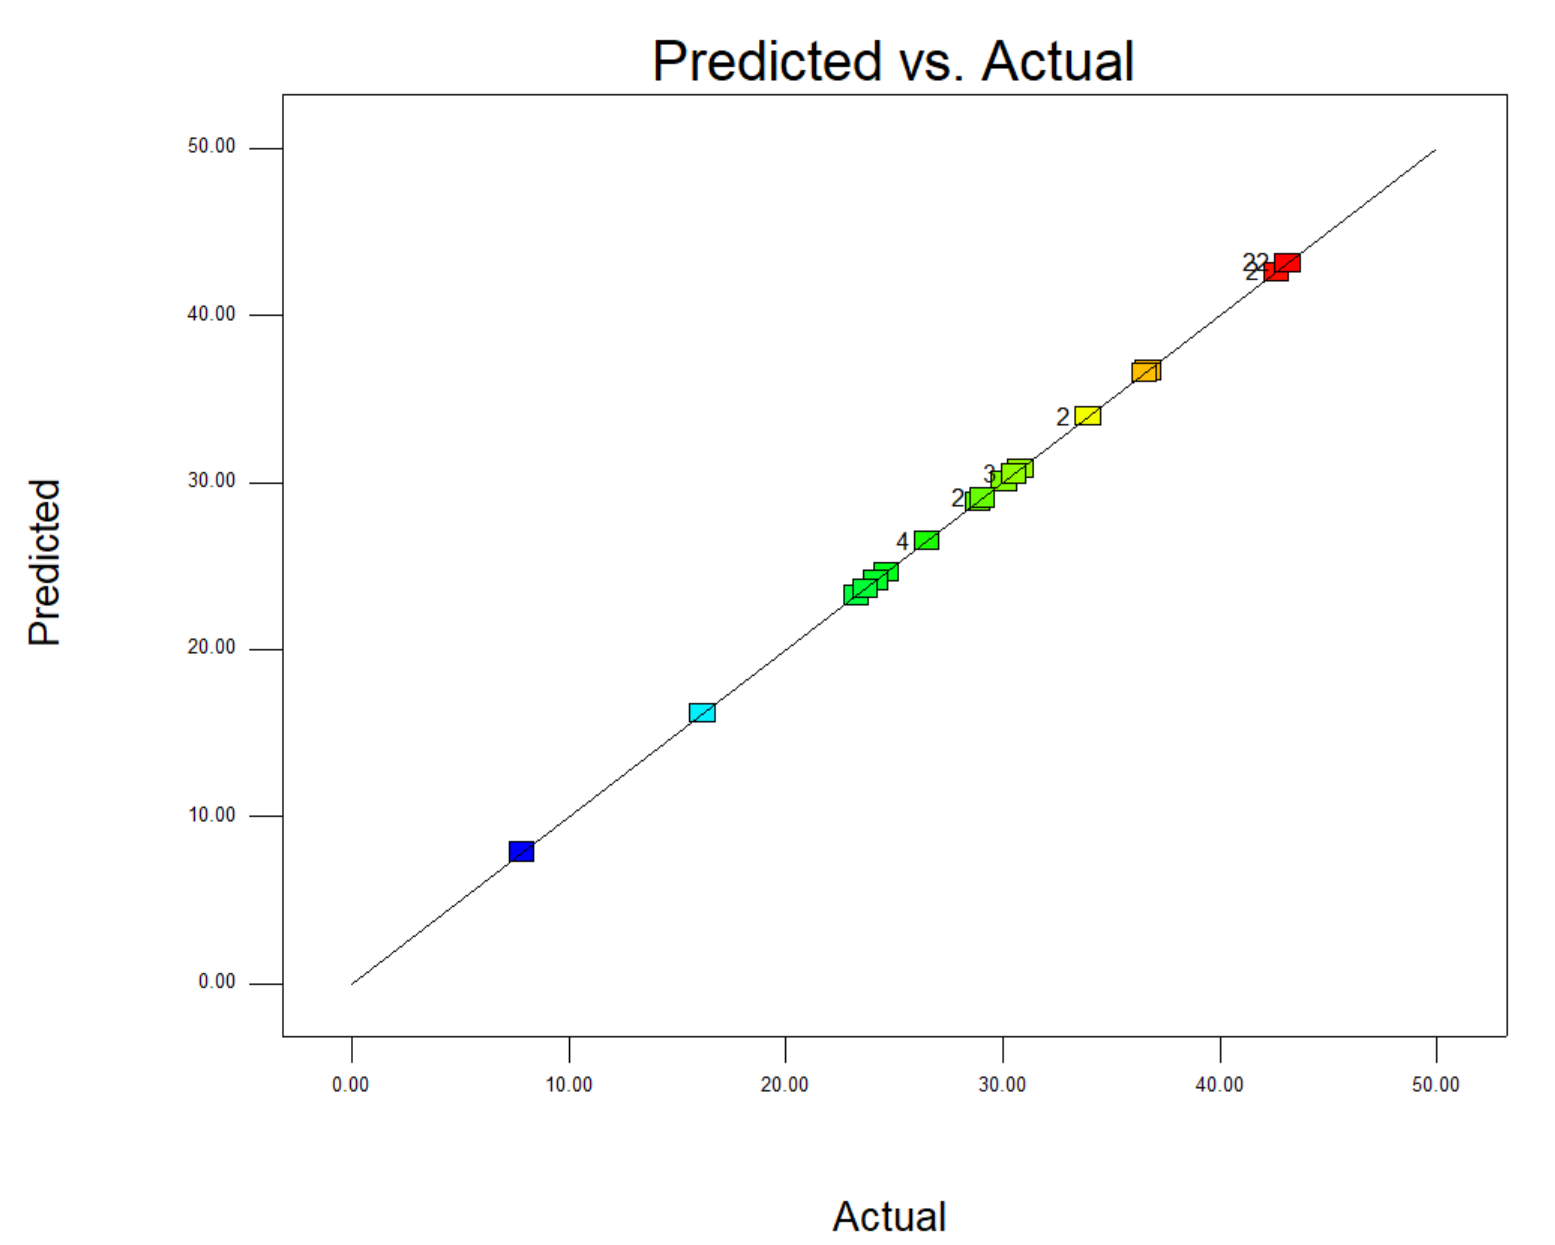
\includegraphics[width=1.0\textwidth]{3_4}
	\caption{响应曲面四次模型的预测值与真实值}
	\label{fig:circuit-diagram1}
\end{figure}
从图34中可以看出,预测值与真实呈现线性关系,这表明预测的精度较高,也即响应曲面四次模型对试验数据的拟合效果较好。


\newpage
\textbf{4.响应曲面}

响应曲面中各参数含义:A-温度,B-Co负载量,C-Co/SiO2和HAP装料比,D-乙醇浓度,E-Co/SiO2和HAP总质量。根据组合原理,我们得到10组响应曲面,即5个自变量两两组合与因变量C4烯烃收率之间的函数图像。图像均呈现凸形,这表明C4烯烃收率具有最大值,下面我们将进行求解。

\begin{figure}[!h]
	\centering
	\begin{minipage}[c]{0.45\textwidth}
		\centering
		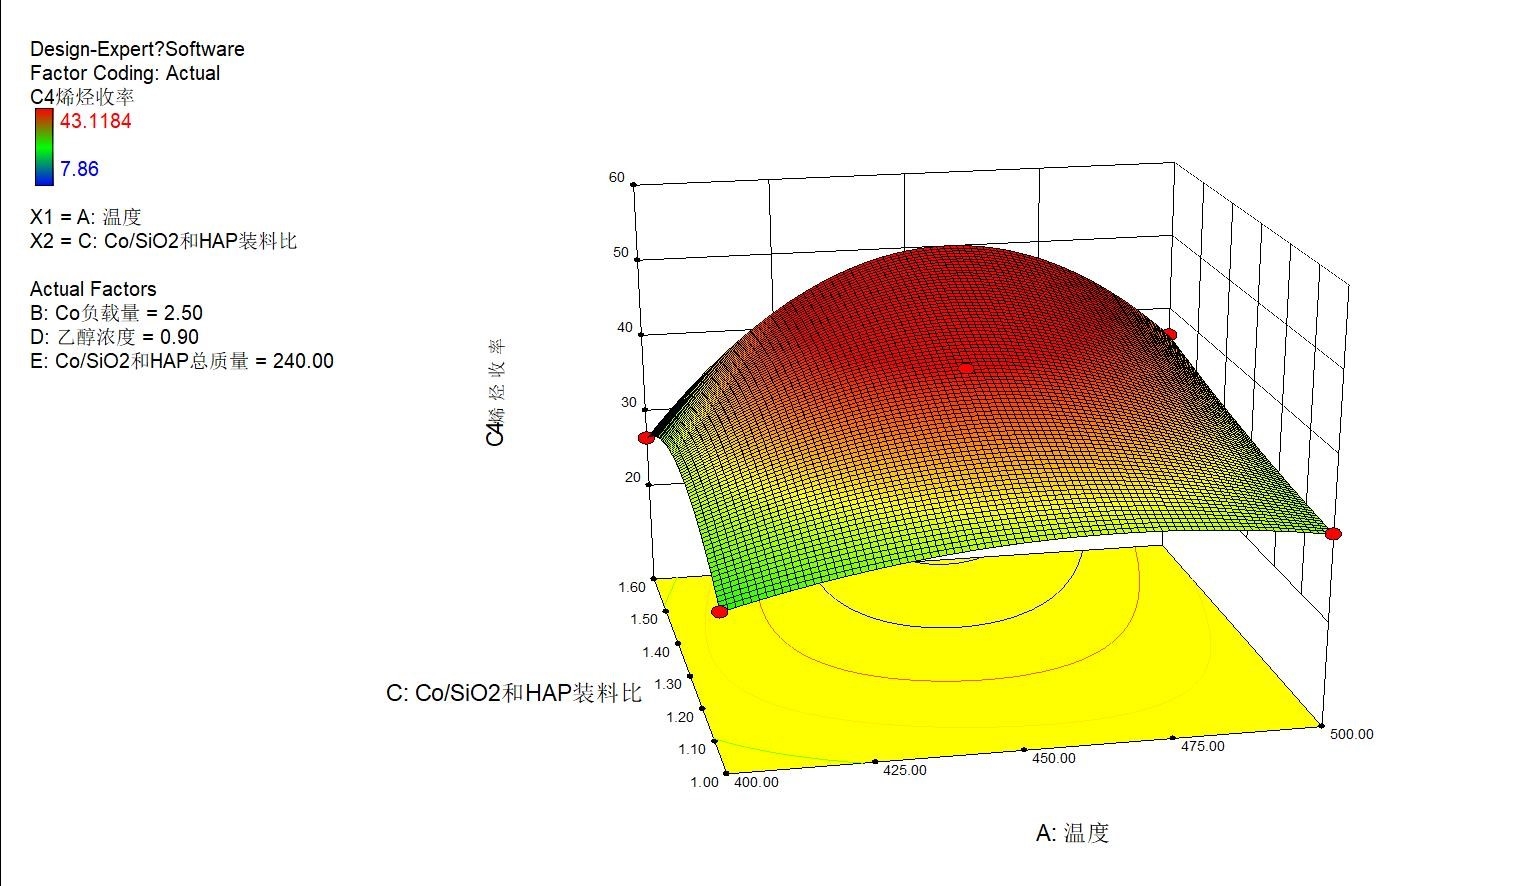
\includegraphics[width=0.95\textwidth]{1}
		\subcaption{A-C响应曲面}
		\label{fig:sample-figure-a}
	\end{minipage}
	\begin{minipage}[c]{0.45\textwidth}
		\centering
		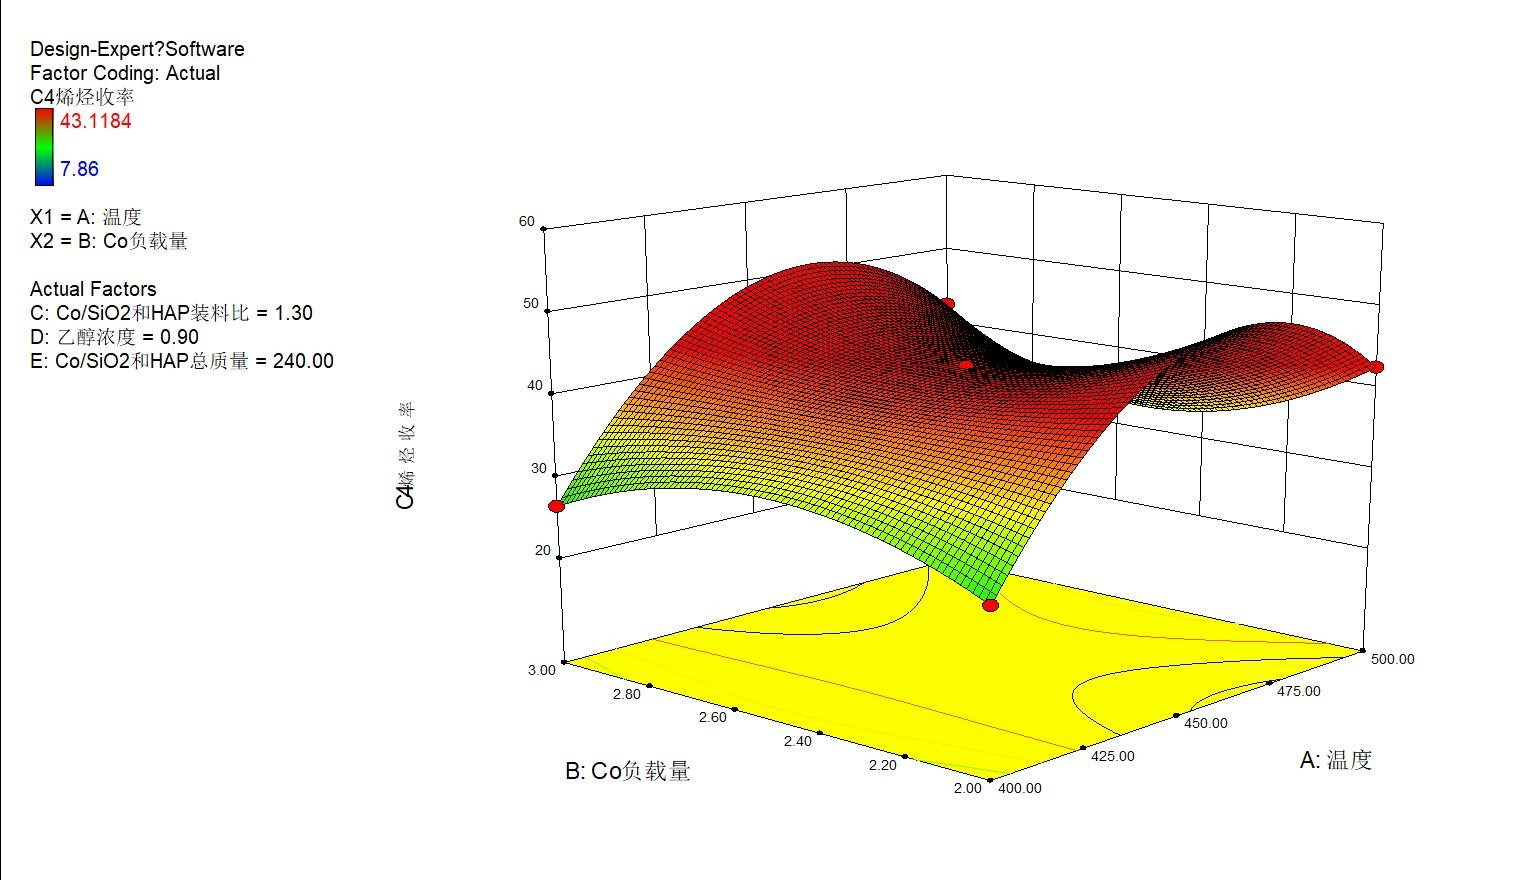
\includegraphics[width=0.95\textwidth]{2}
		\subcaption{A-B响应曲面}
		\label{fig:sample-figure-b}
	\end{minipage}
	\caption{A-BC响应曲面}
	\label{fig:sample-figure}
\end{figure}

\begin{figure}[!h]
	\centering
	\begin{minipage}[c]{0.45\textwidth}
		\centering
		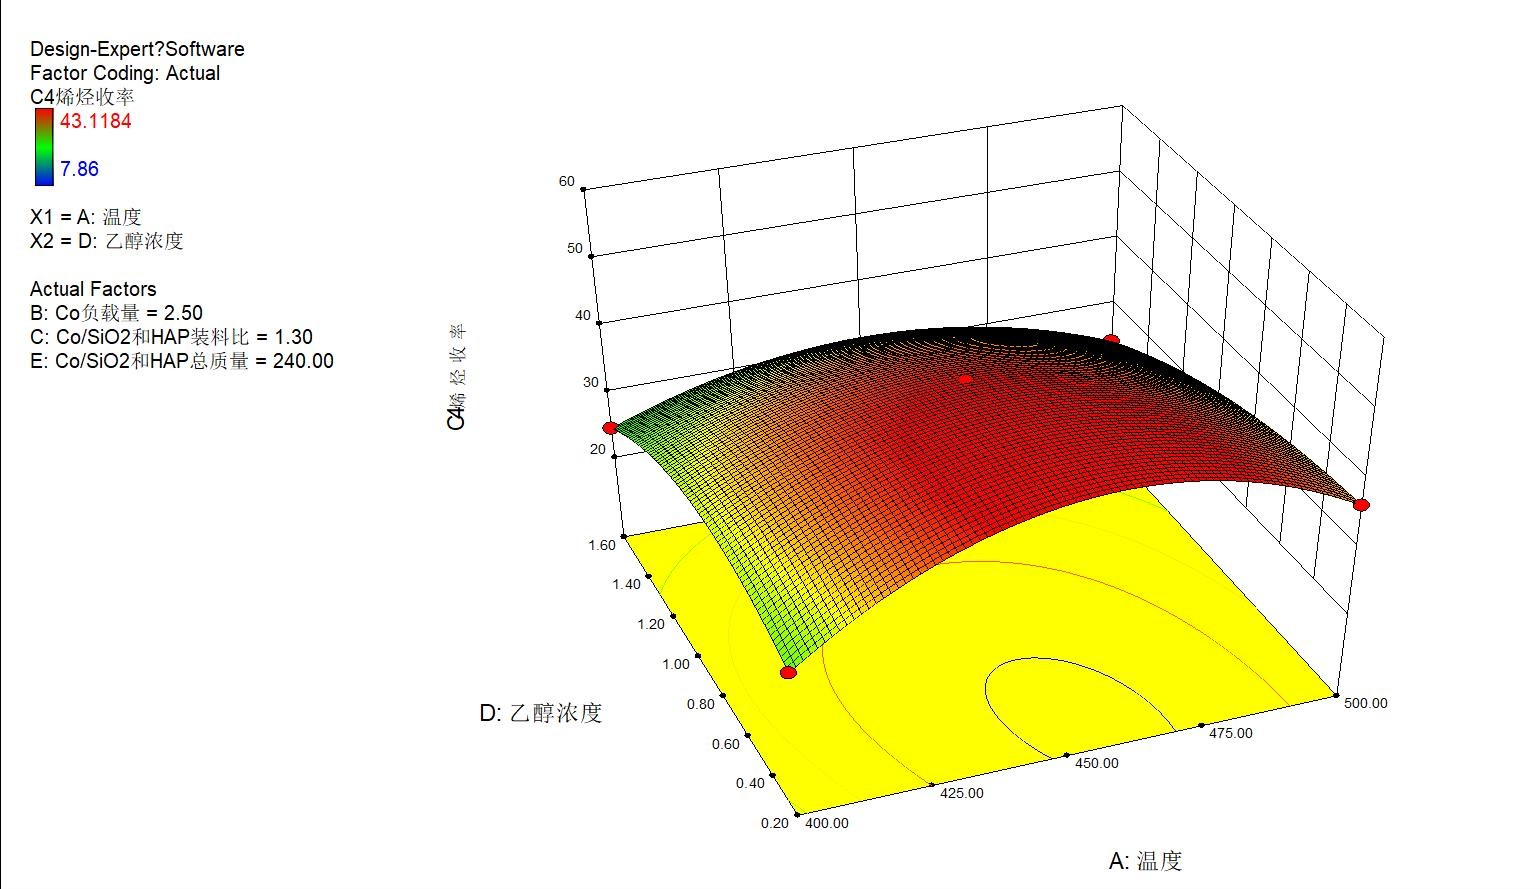
\includegraphics[width=0.95\textwidth]{3}
		\subcaption{A-D响应曲面}
		\label{fig:sample-figure-a}
	\end{minipage}
	\begin{minipage}[c]{0.45\textwidth}
		\centering
		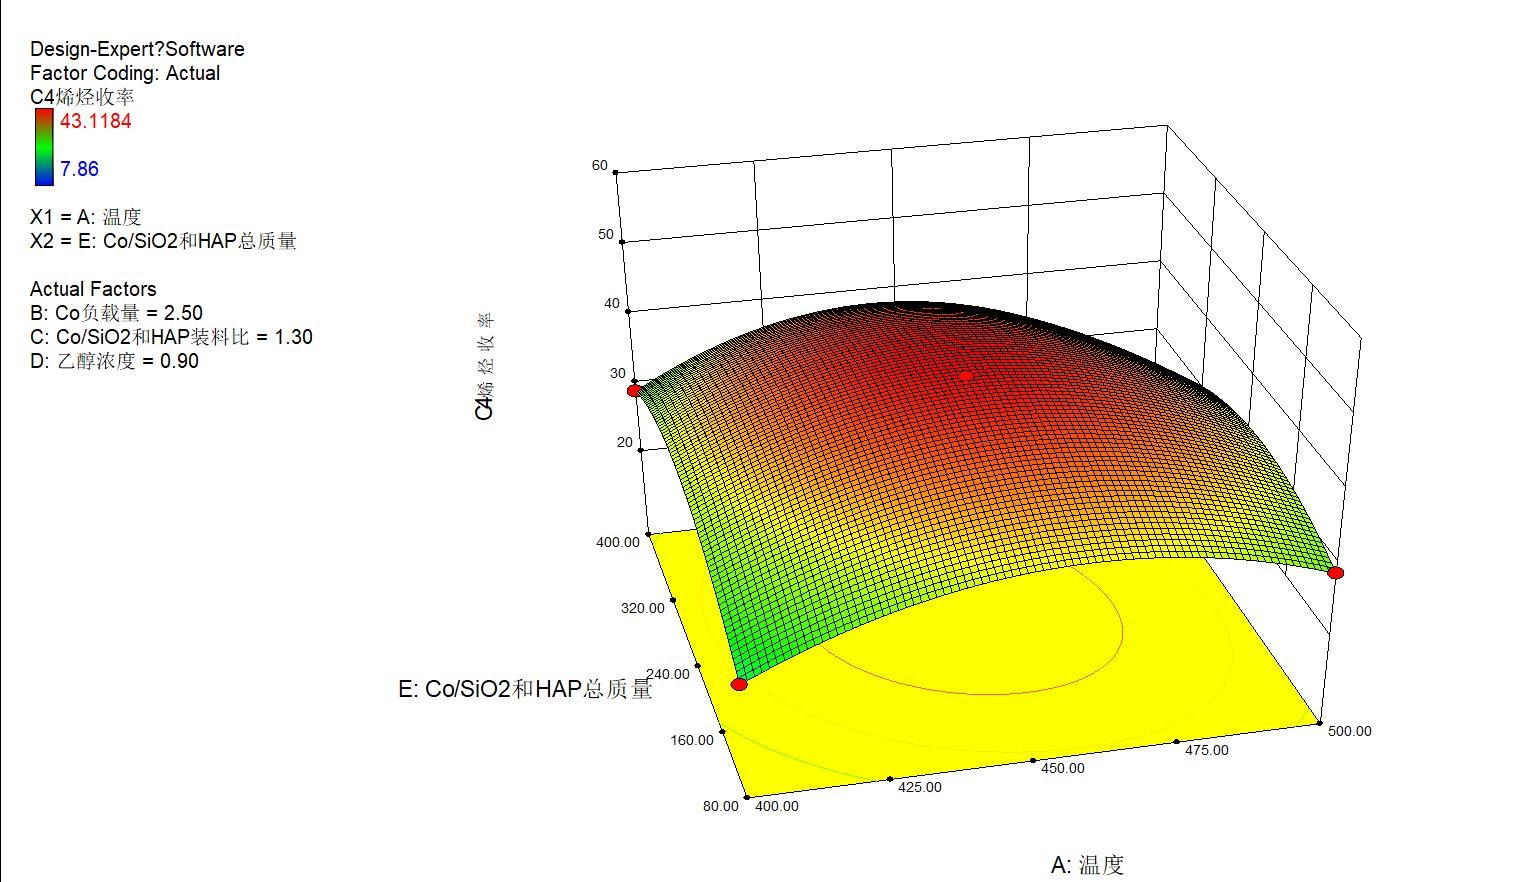
\includegraphics[width=0.95\textwidth]{4}
		\subcaption{A-E响应曲面}
		\label{fig:sample-figure-b}
	\end{minipage}
	\caption{A-DE响应曲面}
	\label{fig:sample-figure}
\end{figure}

\begin{figure}[!h]
	\centering
	\begin{minipage}[c]{0.45\textwidth}
		\centering
		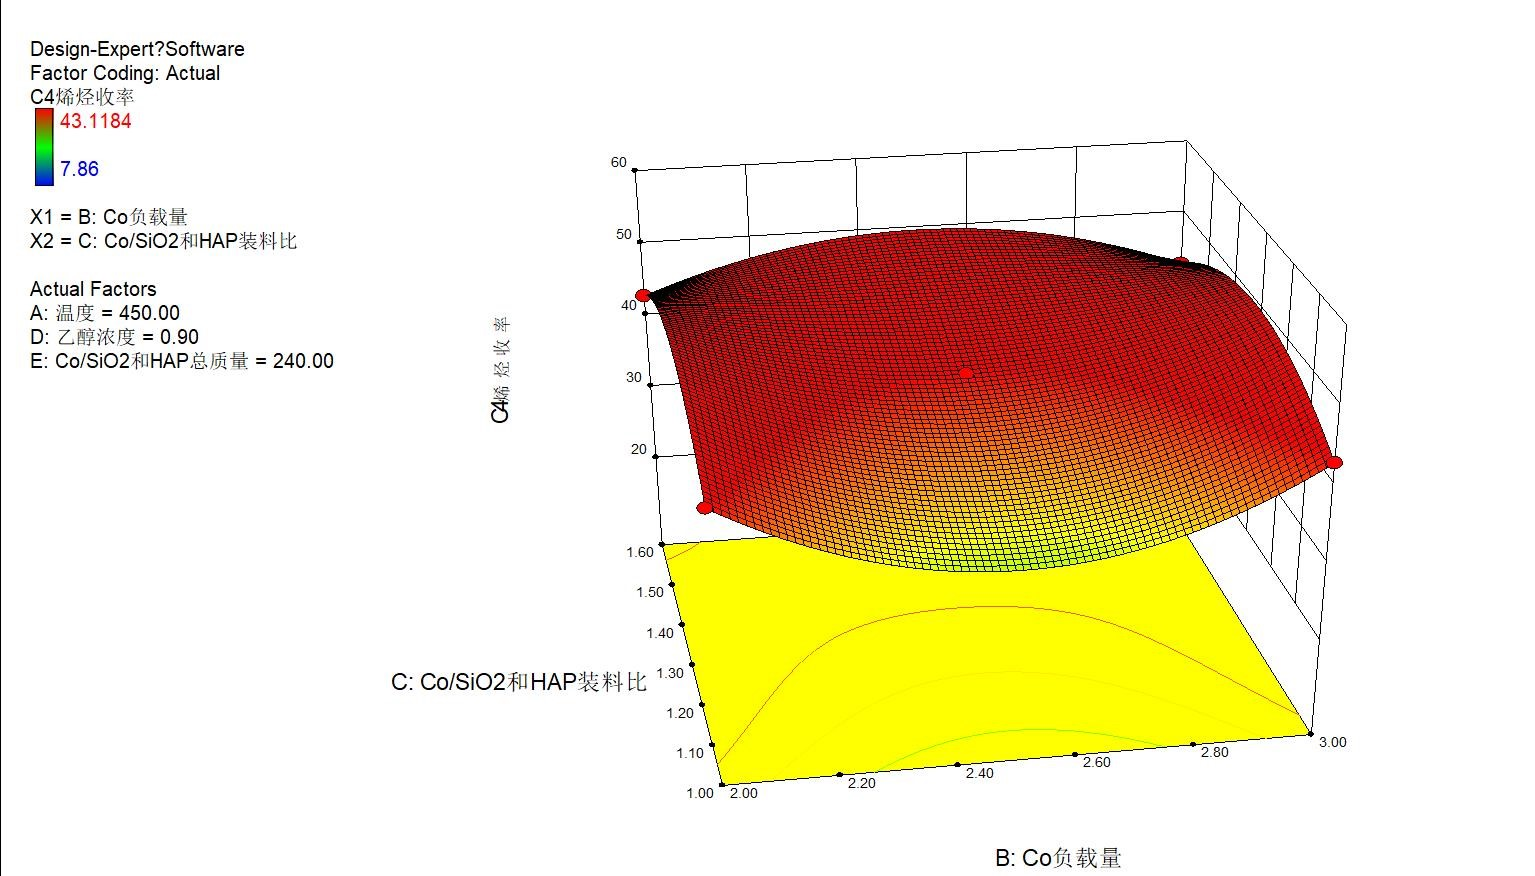
\includegraphics[width=0.95\textwidth]{5}
		\subcaption{B-C响应曲面}
		\label{fig:sample-figure-a}
	\end{minipage}
	\begin{minipage}[c]{0.45\textwidth}
		\centering
		\includegraphics[width=0.95\textwidth]{6}
		\subcaption{B-D响应曲面}
		\label{fig:sample-figure-b}
	\end{minipage}
	\caption{B-CD响应曲面}
	\label{fig:sample-figure}
\end{figure}


\begin{figure}[!h]
	\centering
	\begin{minipage}[c]{0.45\textwidth}
		\centering
		\includegraphics[width=0.95\textwidth]{7}
		\subcaption{B-E响应曲面}
		\label{fig:sample-figure-a}
	\end{minipage}
	\begin{minipage}[c]{0.45\textwidth}
		\centering
		\includegraphics[width=0.95\textwidth]{8}
		\subcaption{C-D响应曲面}
		\label{fig:sample-figure-b}
	\end{minipage}
	\caption{BE-CD响应曲面}
	\label{fig:sample-figure}
\end{figure}


\begin{figure}[!h]
	\centering
	\begin{minipage}[c]{0.45\textwidth}
		\centering
		\includegraphics[width=0.95\textwidth]{9}
		\subcaption{C-E响应曲面}
		\label{fig:sample-figure-a}
	\end{minipage}
	\begin{minipage}[c]{0.45\textwidth}
		\centering
		\includegraphics[width=0.95\textwidth]{10}
		\subcaption{D-E响应曲面}
		\label{fig:sample-figure-b}
	\end{minipage}
	\caption{E-CD响应曲面}
	\label{fig:sample-figure}
\end{figure}

\newpage
\textbf{5.求解催化剂最优组合}

为寻找最优组合,此处的约束条件即为我们在第二问中通过单变量分析方法得到的因素水平。其中需要注意的C4烯烃收率的上下限,默认情况下,它会将输入数据中的最大值作为上限,最小值作为下限。由于我们需要求C4烯烃收率最大值,因此需要更改默认的上限约束。但该上限与模型的合意性(Desirability)成负相关。所谓合意性是一个目标函数,范围从超出限制的零到达到目标的 1。数值优化找到使合意性函数最大化的点。可以通过调整权重或重要性来改变目标的特征。对于多个响应和因素,所有目标都合并为一个合意性函数。

需要注意的是,不要盲目追求非常高的合意性值。该值完全取决于相对于实际最佳值设置的下限和上限的接近程度。优化的目标是找到一组能够满足所有目标的良好条件,而不是达到合意性值 1.0。合意性只是一种寻找最佳值的数学方法。

经多次调节C4烯烃收率的上限,当该值大于53左右时,C4烯烃收率具有稳定的最大值,且合意性随着该值的增大而降低;当该值小于50左右时,C4烯烃收率的最大值与上限相接近,合意性基本接近于1.

\newpage
下面列出当C4烯烃上限为55时的约束条件(图40):
\begin{figure}[!h]
	\centering
	\includegraphics[width=1.0\textwidth]{4_1}
	\caption{响应曲面最优解约束条件}
	\label{fig:circuit-diagram1}
\end{figure}

在此约束条件下,我们共得到54组相互接近的最优解催化剂组合方案,其中合意性最高为0.955180293。
部分数据如下图所示,更多最优组合方案详见“我的支撑材料-最优解组合.csv”:

\begin{figure}[!h]
	\centering
	\includegraphics[width=1.0\textwidth]{4_2}
	\caption{最优催化剂组合方案}
	\label{fig:circuit-diagram1}
\end{figure}
在上述组合方案中,前7种的Co/SiO2和HAP的质量比均为1.00,联系表中的Co/SiO2和HAP质量之和我们可以简单计算出催化剂组合中Co/SiO2和HAP的实际质量。

\subsection{350度下的催化剂最优组合}
与上面所采用的方法一样,我们首先将根据第二问确定因素水平值,然后通过Adaboost回归模型进行计算,并使用design-expert软件进行分析。
约束条件如下所示(图42):

\begin{figure}[!h]
	\centering
	\includegraphics[width=1.0\textwidth]{4_13}
	\caption{低于350度约束条件}
	\label{fig:circuit-diagram1}
\end{figure}


进一步我们分析响应曲面的变化,通过观察我们发现,响应曲面大致分为两种:含有温度的响应曲面和不含温度的响应曲面。
\begin{figure}[!h]
	\centering
	\begin{minipage}[c]{0.45\textwidth}
		\centering
		\includegraphics[width=0.95\textwidth]{5_1}
		\subcaption{含温度的响应曲面}
		\label{fig:sample-figure-a}
	\end{minipage}
	\begin{minipage}[c]{0.45\textwidth}
		\centering
		\includegraphics[width=0.95\textwidth]{5_2}
		\subcaption{未含温度的响应曲线}
		\label{fig:sample-figure-b}
	\end{minipage}
	\caption{350度下两类响应曲面}
	\label{fig:sample-figure}
\end{figure}
在含有温度的响应曲面图像中(图43-a),目标值C4烯烃收率基本随着温度的升高而增大,而与其它变量的关系并不密切。其中当温度小于350度时,增长缓慢;当温度大于350度时,C4烯烃收率的增长速率加快。在未含有温度的响应曲面中,C4烯烃收率与两因变量之间并无明显变化关系,如图43(b)中显示:曲面接近与平面。

因此,可以大胆猜测,当温度小于350度时,C4烯烃收率主要由温度决定,且随温度的升高的增大,而与其它因素之间的关系并不大。为验证该猜想,我们查询了拟合函数:

$C4\text{烯烃收率}	 =
+3.28
+8.17	 * A
+0.000	 * B
+0.000	 * C
-0.84	 * D
+0.35	 * E
+0.000	 * A * B
+0.26	 * A * C
+0.47	 * A * D
+3.08	 * A * E
-0.18	 * B * C
+0.000	 * B * D
+0.000	 * B * E
+0.025	 * C * D
+0.000	 * C * E
+0.35	 * D * E
+5.98	 * A^2
-0.021	 * B^2
-0.021	 * C^2
-0.25	 * D^2
-0.35	 * E^2
+0.000	 * A^2 * B
+0.26	 * A^2 * C
+0.50	 * A^2 * D
+2.73	 * A^2 * E
-3.08	 * A * B^2
-2.82	 * A * C^2
-3.19	 * A * D^2
+0.18	 * B^2 * C
+0.35	 * B^2 * D
+0.018	 * B^2 * E
+0.18	 * B * C^2
+0.000	 * B * D^2
+0.38	 * C^2 * D
+0.018	 * C^2 * E
-0.025	 * C * D^2
-3.41	 * A^2 * B^2
-3.15	 * A^2 * C^2
-2.94	 * A^2 * D^2
-0.14	 * B^2 * C^2
+0.025	 * B^2 * D^2
$

拟合函数中,含有A(温度)的项的系数的绝对值较大,而不含有A的项的系数基本接近于0,这表明我们的初步猜想是正确的。

进一步,我们得到在温度低于350度下最优催化剂组合方案,其中温度接近350度,而C4烯烃收率的最优值接近11.08\%,这与已有试验数据中的特征相符合。详细催化剂组合方案见“我的支撑材料-最优化组合350.csv”.

\begin{figure}[!h]
	\centering
	\includegraphics[width=1.0\textwidth]{4_14}
	\caption{温度低于350度下最优催化剂组合方案(部分)}
	\label{fig:circuit-diagram1}
\end{figure}


\newpage
\section{问题四的模型建立与分析}
\subsection{正交设计试验方案}
第一种方案我们通过进行正交设计的方差分析,从而选择当前最佳的实验方案。

影响C4烯烃收率的因素包括Co负载量、Co/SiO2质量(mg)、HAP质量(mg)、乙醇浓度(ml/min)、温度、装料方式,催化剂中是否加HAP将它们分别记录为影响因素A,B,C,D,E,F,G。

根据已有实验数据,可知
Co负载量可为0.5wt\%,1wt\%,2wt\%,5wt\%,分别记为A1,A2,A3,A4,共4个水平; Co/SiO2质量可为10, 25,33,50,67,75,100,200mg,分别记录为B1,B2,B3,B4,B5,B6,B7,B8,共八个水平;HAP质量可为10,25,33,50,67,75,90,200mg,依次记录为C1,C2,C3,C4,C5,C6,C7,C8,共8个水平;乙醇浓度可为0.3,0.9, 1.68,2.1ml/min,分别记录为D1,D2,D3,D4,共4个水平;温度可为250,275,300,325,350,400,450分别记录为E1,E2,E3,E4,E5,E6,E7,共7个水平;装料方式有A、B两种,分别记录为F1,F2,共两个水平;催化剂中是否加HAP,加则记录为G1,不加则记录为G2,共两个水平。

首先对实验室数据进行处理,对每一个影响因素,将其数值信息从小到大转化成相应的水平数码数,如0.5wt\%,1wt\%,2wt\%,5wt\%分别对应于水平数1,2,3,4。


采用正交设计的方差分析法,本题总共开展了114次实验,把C4烯烃收率作为因变量,记录C4烯烃收率(\%)分别为$y_1,y_2,y_3,...,  y_{114}$,则总离差的平方和$SS_T=\sum_{i=1}^{114}{(y_i-\vec{y})^2}$,$\vec{y}=\frac{1}{114}\sum_{i=1}^{114}y_i$。

一般地,$SS_T$的分解公式为:
\begin{equation*}
	SS_T = SS_1 + SS_2 + ... + SS_r
\end{equation*}
其中$SS_j(j = 1,2,...,r)$是正交表$L_n(p^r)$中第$j$列因素的离差平方和。

使用公式${SS}_j=\frac{{k1}^2+{k2}^2+...{ks}^2}{m}-\frac{(\sum_{i=1}^{n}yi)^2}{n}$,(其中$m$为第$j$列因素1出现的次数,$n$为实验总数,$s$为该列的数码数)来计算每个因素的离差平方和。

得出离差平方和之后,进一步确定各个因素离差平方和的自由度${df}_i$,总离差的自由度${df}_E$等于实验次数减1,每一列的自由度${df}_i$等于水平数减1,交互作用的自由度等于两个因素的自由度之积。

在上述操作的基础上,计算F检验统计量,进行F检验。其计算公式为:
\begin{equation}
		F_{j}=\frac{S S_{j} / d f_{j}}{S S_{E} / d f_{E}} \sim F\left(d f_{j}, d f_{E}\right)
\end{equation}
按照F检验法判断有关因素的影响是否显著,取显著性水平为0.05,置信区间为0.95。计算得到的异方差检验表和方差分析表如下图所示(图45):
\begin{figure}[!h]
	\centering
	\begin{minipage}[c]{0.48\textwidth}
		\centering
		\includegraphics[height=0.2\textheight]{4_3}
		\subcaption{异方差检验表}
	\end{minipage}
	\begin{minipage}[c]{0.48\textwidth}
		\centering
		\includegraphics[height=0.2\textheight]{4_4}
		\subcaption{方差分析表}
	\end{minipage}
	\caption{异方差检验表和方差分析表}
\end{figure}

\newpage
通过上述正交设计数据多因素方差分析表可知,对于显著水平$\alpha=0.05$  ,有:
\begin{itemize}
	\item 对于Co负载量、因为其显著性0.00<0.05,故它的影响显著;
	\item 对于CoSiO2质量,因为其显著性0<0.05,故它显著;
	\item 对于HAP质量, 因为其显著性0.046<0.05,故它的影响显著;
	\item 对于乙醇浓度,因为其显著性0.001<0.05,故它显著;
	\item 对于温度,因为其显著性0.000<0.05,故它显著;
	\item 对于有无HAP,因为其显著性0.239>0.05,故它不显著;
	\item 对于装料方式,因为其显著性0.609>0.05,故它不显著。	
\end{itemize}

Co负载量、CoSiO2质量、HAP质量、乙醇浓度,温度对因变量C4烯烃收率具有显著性的影响。使用SPSS生成参数估算值列表,选择标准误差最低对应的水平数。

计算参数估计值如下表所示(图46):(参数为1表示第一种,参数为2表示第2种……,对应的具体数值见上述文档)
\begin{figure}[!h]
	\centering
	\begin{minipage}[c]{0.48\textwidth}
		\centering
		\includegraphics[height=0.2\textheight]{4_5}
		\subcaption{参数估计值}
	\end{minipage}
	\begin{minipage}[c]{0.48\textwidth}
		\centering
		\includegraphics[height=0.2\textheight]{4_6}
		\subcaption{参数估计值}
	\end{minipage}
	\caption{参数估计值}
\end{figure}


由参数估计值可知:
\begin{itemize}
	\item 对于Co负载量,Co负载量=A2时的显著性最小且标准误差为7.715也为最小,因此,备选试验方案中Co负载量取1wt%。
	\item 对于CoSiO2质量,CoSiO2质量取B5和B3时显著性为0.005,标准误差为2.656,标准误差为所有组中最低,Co/SiO2质量取33mg或67mg,为节省资源,Co/SiO2质量取33mg。
	
	\item 对于HAP质量,剔除无效数据,其值取C4时数据有效,显著性为0.83,因此HAP质量取50mg。
	
	\item 对于乙醇浓度这个指标,其值为D3时对应的标准误差为1.829,因此乙醇浓度应取1.68ml/min。
	
	\item 对于温度,当温度水平数为D5时其标准误差为5.135,达到最小,故温度取350
	
	\item 对于装料方式,装料方式不显著,可任意选取,选取装料方式I.
	
	\item 对于是否在催化剂中加HAP,由于不显著可任意选取,因此,选择在催化剂中加入HAP。	
\end{itemize}

总上所述,实验方案设计如下:
\begin{figure}[!h]
	\centering
	\includegraphics[width=0.8\textwidth]{4_7}
	\caption{正交设计方案}
	\label{fig:circuit-diagram1}
\end{figure}



\subsection{均匀试验设计方案}
思路二是采用均匀试验设计方案设计试验。指标变量(因变量)指定为C4烯烃收率,用Y表示,影响Y值的m个因素变量因素变量用$x_1,x_2,...,x_m$表示,对已知的样本观测值利用最小二乘法估计系数$b_0,b_1,...,b_n$,进而得到多元线性回归方程:
\begin{equation*}
	\hat{y}=b_{0}+b_{1} x_{1}+\cdots+b_{m} x_{m}
\end{equation*}

并用F检验法做回归的显著性检验。取$\alpha=0.1$,将自变量:是否有HAP剔除,多元回归的输出结果如下表所示:
\begin{figure}[!h]
	\centering
	\includegraphics[width=1.0\textwidth]{4_8}
	\caption{多元回归结果}
	\label{fig:circuit-diagram1}
\end{figure}



由分析结果因变量Y可表示为$Y=-0.7X_A+0.023X_B+0.022X_C-1.713X_D+0.129X_E+4.021X_F$.
为了提高方程的显著性,将自变量中显著性远大于0.1的两个自变量Co/SiO2质量(\%)和HAP质量剔除,重新进行多元回归分析:
\begin{figure}[!h]
	\centering
	\includegraphics[width=0.8\textwidth]{4_9}
	\caption{多元回归分析}
	\label{fig:circuit-diagram1}
\end{figure}



所得回归模型的显著性检验的P值小于0.1,认为显著性良好。由表格系数(图49)可知回归方程为:

$Y=-0.031X_A-3.785X_D+0.128X_E+4.645X_F$

要使因变量C4烯烃收率最大,则自变量$X_E,X_F$取最大值,$X_A,X_D$取最小值。其它被剔除的变量我们认为对结果产生的显著性不大,从节省资源的角度考虑取相应的值。

综上所述,实验方案设计为:
\begin{figure}[!h]
	\centering
	\includegraphics[width=1.0\textwidth]{4_10}
	\caption{均匀试验设计方案}
	\label{fig:circuit-diagram1}
\end{figure}


\subsection{验证最优催化剂组合}
第三个实验方案是用第三问得出的优化结果,用于测试和验证优化的结果是否符合预期,从而验证模型的准确度。
\begin{figure}[!h]
	\centering
	\includegraphics[width=0.8\textwidth]{4_19}
	\caption{验证最优催化剂组合}
	\label{fig:circuit-diagram1}
\end{figure}




\subsection{进一步分析C4烯烃收率与乙醇浓度关系}
在第二问使用A7、A8、A9、A12组数据探究乙醇浓度与C4烯烃收率的关系时,发现随着乙醇浓度的增大,C4烯烃收率呈下降趋势,基于探索随着乙醇浓度的继续增大后,C4烯烃收率会发生何种变化,拟在原有实验数据的基础上增大乙醇浓度,并与现有实验数据进行对照。将温度设为350度便于观察曲线的走势。实验方案如下:
\begin{figure}[!h]
	\centering
	\includegraphics[width=1.0\textwidth]{4_11}
	\caption{C4烯烃收率与乙醇浓度关系探求设计方案}
	\label{fig:circuit-diagram1}
\end{figure}




\subsection{催化剂HAP对照设计}
实验数据中A11组中催化剂没有HAP而是用石灰砂代替,但是其他组中有没有可以与A11组形成对照的组合,以至于无法对比分析有HAP和没有HAP对C4的烯烃化率造成的影响。因此,从第三问所求出的最适温度范围中抽取C4烯烃收率最高对应的温度点468.22作为最佳温度,催化剂中添加HAP,其余自变量取值与A11中的实验数据相同,便于形成对照。因此,实验方案设计如下:

\begin{figure}[!h]
	\centering
	\includegraphics[width=1.0\textwidth]{4_12}
	\caption{催化剂HAP对照设计方案}
	\label{fig:circuit-diagram1}
\end{figure}




\newpage
\section{模型的评价}
\subsection{拟合模型}
\subsubsection{高斯拟合模型}
\textbf{优点:}

对数据点集进行函数逼近,能够较好地拟合出化学反应中各物质含量的动态变化。

\textbf{缺点:}

当点集出现波动的情况,高斯拟合的效果存在瑕疵,并且函数高度对称,难以拟合对称性较差的数据。

\subsubsection{指数拟合模型}
\textbf{优点:}

能够较好的反应很多化学反应的过程,能有效地反应非线性过程。

\textbf{缺点:}

函数单调性唯一,不利于拟合单调性发生变化的函数。

\subsubsection{多项式拟合模型}
\textbf{优点:}

应用广泛,适用性强,泛用性广,拟合精度高。

\textbf{缺点:}

容易出现过拟合现象。

\subsection{组合优化-预测模型}
\subsubsection{Adaboost回归模型}
\textbf{优点:}
\begin{itemize}
	\item 在建模过程中使用Adaboost构建的决策树能够保证有较高的精度。
	\item 模型充分考虑了化学反应过程中每一个影响因素所占据的权重。
	\item 测试数据集时,运行速度比较快
	\item 便于可视化分析,从而发现变量之间隐藏的规律
\end{itemize}

\textbf{缺点:}

不易确定AdaBoost迭代次数。

\subsubsection{RSM模型}
\textbf{优点}
\begin{itemize}
	\item 克服了正交试验只能给出最佳因素水平组合, 而无法找出整个区域上因素的最佳组合和响应值的最优值的缺陷。
	\item 可以将多因子试验中因素与试验结果的关系用
	多项式拟合, 将因子与试验结果的关系函数化, 因
	此, 可对函数的面进行分析, 研究因子与响应值之
	间、因子与因子之间的相互关系, 并进行优化。
\end{itemize}

\textbf{缺点}

需要试验区域已接近最优区域,否则误差较大。


\subsubsection{BBD模型}
\textbf{优点}
\begin{itemize}
	\item 试验次数较少,且可以对因素间可能的交互作用进行考察;
	\item 所有因素水平没有同时为最大或最小,避免了极值时可能出现的不理想结果;
	\item 考虑了实验的随机误差;
	\item 使用了数学模型及一系列检验,有利于对参数影响效应的准确评估;
\end{itemize}

\textbf{缺点}

BBD过分依靠计算机进行的试验设计和数据处理,对于如何生成良好的或稳定的设计方案,还不存在通用的基本原则,有时尚需要与其他方法联合来分析因子系统的最佳条件。


\subsection{分析模型}
\subsubsection{Spearman相关分析模型}
\textbf{优点}

模型利用单调方程评价变量的相关性,能分析非线性相关性,解释变量之间的关联程度。

\subsubsection{量纲分析模型}
\textbf{优点}

能够较为方便地建立起没有理论疑点的模型,能够挖掘变量的联系。

\textbf{缺点}

初等建模方法,使用存在局限。

\subsection{设计模型}
\subsubsection{正交设计的方差分析模型}
\textbf{优点:}
\begin{itemize}
	\item 能够区别出试验结果的差异是由因素水平的改变所引起,还是由试验的随机波动所引起。
	\item 能够确定哪些因素及因素之间的交互作用对试验指标有显著性影响。
	\item 能够对试验因素做出合理且有效的安排
	\item 能够在多个自变量存在的试验中选出最优的实验方案
\end{itemize}

\textbf{缺点:}
\begin{itemize}
	\item 在挑选代表点时要求数据点具有“均匀分散、整齐可比”的特点;
	\item 只适用于影响因素的水平数较小的情况,若水平数较小,则需要进行多次试验,且难以得出正确的结果
\end{itemize}

\subsection{均匀实验设计模型}
\textbf{优点}

对于水平数较大的情况,能够在较少的试验次数的基础上得出精度较高的结果。

\newpage
%参考文献
\begin{thebibliography}{9}%宽度9
	\bibitem[1]{1} 吕绍沛. 乙醇偶合制备丁醇及C\_4烯烃[D].大连理工大学,2018.
	
	\bibitem[2]{2}
	徐燕.SPSS软件在数学建模竞赛中的应用实践[J].教育教学论坛,2020(23):331-333.
	
	\bibitem[3] {3} 唐冲,惠辉辉.基于Matlab的高斯曲线拟合求解[J].计算机与数字工程,2013,41(08):1262-1263+1297.
	
	\bibitem[4]{4} 张国秋,王文璇.均匀试验设计方法应用综述[J].数理统计与管理,2013,32(01):89-99.
	
	\bibitem[5] {nb} 姜启源,谢金星,叶俊,数学模型,高等教育出版社,2011.3.6
\end{thebibliography}


\newpage
%附录
\begin{appendices}
	
\section{支撑材料}
\begin{itemize}
	\item 代码.rar
	\begin{itemize}
		\item Co拟合计算.m
		\item 催化剂质量之和拟合计算.m
		\item 附件二拟合计算.m
		\item 乙醇浓度拟合计算.m
		\item 装料比拟合计算.m
		\item 组内温度分析.m
	\end{itemize}
	\item design-expert.rar: design-expert V8.0.6.1 源文件及相关数据
	\item 问题1\_温度关系.docx
	\item 最优化组合305.csv
	\item 最优解组合.csv
\end{itemize}


\section{Co拟合计算.m--matlab 源程序}

\begin{lstlisting}[language=matlab]
%负载拟合

%数据处理
A=xlsread('1.xlsx'); %去除表头的数据文件
at=A(1:3,1);
at=[at;A(5,1)];
az=A(1:3,2);
az=[az;A(5,2)];
ax=A(1:3,4);
ax=[ax;A(5,4)];
as=az.*ax;
bt=A(6:8,1);
bt=[bt;A(10,1)];
bz=A(6:8,2);
bz=[bz;A(10,2)];
bx=A(6:8,4);
bx=[bx;A(10,4)];
bs=bz.*bx;
ct=A(18:20,1);
ct=[ct;A(22,1)];
cz=A(18:20,2);
cz=[cz;A(22,2)];
cx=A(18:20,4);
cx=[cx;A(22,4)];
cs=cz.*cx;
dt=A(30:33,1);
dz=A(30:33,2);
dx=A(30:33,4);
ds=dz.*dx;
bl=[1,2,0.5,5];
sl=[];
for i=1:1:4
sl=[sl;as(i),bs(i),cs(i),ds(i)];  
end
ss1=sl(1,:);
ss2=sl(2,:);
ss3=sl(3,:);
ss4=sl(4,:);

%函数调用
[r1,r2]=e1(bl,ss1,bl,ss2,bl,ss3,bl,ss4);

%函数体
function [fitresult2, gof2] = e1( x, y, x1, y1, x2, y2, x3, y3) 

[xData, yData] = prepareCurveData( x, y );
[xData1, yData1] = prepareCurveData( x1, y1 );
[xData2, yData2] = prepareCurveData( x2, y2 );
[xData3, yData3] = prepareCurveData( x3, y3 );

%高斯拟合设置
ft = fittype( 'gauss1' );
opts = fitoptions( 'Method', 'NonlinearLeastSquares' );
opts.Display = 'Off';
opts.Lower = [-Inf -Inf 0];
opts.StartPoint = [0.497 325 53.840127518332];

%拟合
[fitresult, gof] = fit( xData, yData, ft, opts );
[fitresult1, gof1] = fit( xData1, yData1, ft, opts );
[fitresult2, gof2] = fit( xData2, yData2, ft, opts );
[fitresult3, gof3] = fit( xData3, yData3, ft, opts );

%数据显示
h = plot( fitresult, xData, yData,'*');
hold on;
title('拟合曲线图' );
set(h,'LineWidth',1.5,'color',[0 0.59 0.53],'Markersize',5);
h1 = plot( fitresult1, xData1, yData1,'*');
hold on;
set(h1,'LineWidth',1.5,'color',[1 0.34 0.13],'Markersize',5);
h2 = plot( fitresult2, xData2, yData2,'*');
hold on;
set(h2,'LineWidth',1.5,'color',[0.13 0.59 0.95],'Markersize',5);
h3 = plot( fitresult3, xData3, yData3,'*');
hold on;
set(h3,'LineWidth',1.5,'color',[0.43 0.39 0.65],'Markersize',5);
b1=2.709;
b2=2.561;
b3=2.271;
b4=2.237;
ylim=get(gca,'Ylim');
plot([b1,b1],ylim,'--','color',[0 0.59 0.53]); 
hold on;
plot([b2,b2],ylim,'--','color',[1 0.34 0.13]); 
hold on;
plot([b3,b3],ylim,'--','color',[0.13 0.59 0.95]); 
hold on;
plot([b4,b4],ylim,'--','color',[0.43 0.39 0.65]); 
hold on;
set(gcf,'unit','centimeters','position',[5 5 25 15]);
xlabel( 'Co负载量', 'Interpreter', 'none' );
ylabel( 'C4烯烃收率', 'Interpreter', 'none' );
set(gca,'fontsize',11.5,'fontweight','normal');
legend( ' ', '250℃',' ','275℃',' ','300℃',' ','350℃', 'Location', 'NorthWest', 'Interpreter', 'none' );
grid on
end
 \end{lstlisting}

\section{组内温度分析.m--matlab 源程序}
\begin{lstlisting}[language=matlab]
%组内温度分析

%数据处理
A=xlsread('1.xlsx'); %去除表头的数据文件
Astart=109;
Aend=114;
t=A(Astart:Aend,1);
t=t.';
zhl=A(Astart:Aend,2)/100;
zhl=zhl.';
xzx=A(Astart:Aend,4)/100;
xzx=xzx.';
sl=zhl.*xzx;

%函数调用
e1(t, zhl, t, xzx, t, sl );

%Spearman系数计算
Spearman_zhl= corr(t.', zhl.', 'type' , 'Spearman')
Spearman_xzx= corr(t.', xzx.', 'type' , 'Spearman')
Spearman_sl= corr(t.', sl.', 'type' , 'Spearman')

%拟合函数定义
function [fitresult, gof] = e1( x, y, x1, y1, x2, y2) 

[xData, yData] = prepareCurveData( x, y );
[xData1, yData1] = prepareCurveData( x1, y1 );
[xData2, yData2] = prepareCurveData( x2, y2 );

%拟合函数参数设定
ft = fittype( 'gauss1' );
opts = fitoptions( 'Method', 'NonlinearLeastSquares' );
opts.Display = 'Off';
opts.Lower = [-Inf -Inf 0];
opts.StartPoint = [0.497 325 53.840127518332];

%拟合
[fitresult, gof] = fit( xData, yData, ft, opts );
[fitresult1, gof1] = fit( xData1, yData1, ft, opts );
[fitresult2, gof2] = fit( xData2, yData2, ft, opts );

%图像显示
h = plot( fitresult, xData, yData);
hold on;
title('B7组目标数据与温度拟合曲线图' );
axis([240,410,0,0.7]);
set(gcf,'unit','centimeters','position',[5 5 25 15]);
set(h,'LineWidth',1.5,'color',[0 0.59 0.53],'Markersize',10);
h1 = plot( fitresult1, xData1, yData1);
hold on;
set(h1,'LineWidth',1.5,'color',[1 0.34 0.13],'Markersize',10);
h2 = plot( fitresult2, xData2, yData2);
hold on;
set(h2,'LineWidth',1.5,'color',[0.13 0.59 0.95],'Markersize',10);
legend( '乙醇转化率实际数据', '乙醇转化率拟合曲线','C4烯烃选择性实际数据','C4烯烃选择性拟合曲线','C4烯烃收率实际数据','C4烯烃收率拟合曲线', 'Location', 'NorthWest', 'Interpreter', 'none' );
% Label axes
xlabel( '温度/℃', 'Interpreter', 'none' );
ylabel( '对应比率', 'Interpreter', 'none' );
set(gca,'fontsize',11.5,'fontweight','normal');
grid on
end	
\end{lstlisting}	

\section{装料比拟合计算.m--matlab 源程序}
\begin{lstlisting}[language=matlab]
%装料比拟合

%数据处理
A=xlsread('1.xlsx'); %去除表头的数据文件
at=A(60:64,1);
az=A(60:64,2);
ax=A(60:64,4);
as=az.*ax/100;
bt=A(65:69,1);
bz=A(65:69,2);
bx=A(65:69,4);
bs=bz.*bx/100;
ct=A(70:74,1);
cz=A(70:74,2);
cx=A(70:74,4);
cs=cz.*cx/100;
bl=[1,2.03,0.49];
sl=[];
for i=1:1:5
sl=[sl;as(i),bs(i),cs(i)];  
end
ss1=sl(1,:);
ss2=sl(2,:);
ss3=sl(3,:);
ss4=sl(4,:);
ss5=sl(5,:);

%函数调用
e1(bl,ss1,bl,ss2,bl,ss3,bl,ss4,bl,ss5);
function [fitresult, gof] = e1( x, y, x1, y1, x2, y2, x3, y3, x4, y4) 

[xData, yData] = prepareCurveData( x, y );
[xData1, yData1] = prepareCurveData( x1, y1 );
[xData2, yData2] = prepareCurveData( x2, y2 );
[xData3, yData3] = prepareCurveData( x3, y3 );
[xData4, yData4] = prepareCurveData( x4, y4 );

%拟合函数参数设定
ft = fittype( 'gauss1' );
opts = fitoptions( 'Method', 'NonlinearLeastSquares' );
opts.Display = 'Off';
opts.Lower = [-Inf -Inf 0];
opts.StartPoint = [0.497 325 53.840127518332];

%拟合
[fitresult, gof] = fit( xData, yData, ft, opts );
[fitresult1, gof1] = fit( xData1, yData1, ft, opts );
[fitresult2, gof2] = fit( xData2, yData2, ft, opts );
[fitresult3, gof3] = fit( xData3, yData3, ft, opts );
[fitresult4, gof4] = fit( xData4, yData4, ft, opts );

%图像显示
h = plot( fitresult, xData, yData,'*');
hold on;
title('拟合曲线图' );
set(h,'LineWidth',1.5,'color',[0 0.59 0.53],'Markersize',5);
h1 = plot( fitresult1, xData1, yData1,'*');
hold on;
set(h1,'LineWidth',1.5,'color',[1 0.34 0.13],'Markersize',5);
h2 = plot( fitresult2, xData2, yData2,'*');
hold on;
set(h2,'LineWidth',1.5,'color',[0.13 0.59 0.95],'Markersize',5);
h3 = plot( fitresult3, xData3, yData3,'*');
hold on;
set(h3,'LineWidth',1.5,'color',[0.43 0.39 0.65],'Markersize',5);
h4 = plot( fitresult4, xData4, yData4,'*');
hold on;
set(h4,'LineWidth',1.5,'color',[0.63 0.39 0.35],'Markersize',5);
ylim=get(gca,'Ylim');
plot([1.393,1.393],ylim,'--','color',[0 0.59 0.53]); 
hold on;
plot([1.328,1.328],ylim,'--','color',[1 0.34 0.13]); 
hold on;
plot([1.353,1.353],ylim,'--','color',[0.13 0.59 0.95]); 
hold on;
plot([1.367,1.367],ylim,'--','color',[0.43 0.39 0.65]); 
hold on;
plot([1.225,1.225],ylim,'--','color',[0.63 0.39 0.35]); 
hold on;
set(gcf,'unit','centimeters','position',[5 5 25 15]);
xlabel( '装料比', 'Interpreter', 'none' );
ylabel( 'C4烯烃收率/%', 'Interpreter', 'none' );
set(gca,'fontsize',11.5,'fontweight','normal');
legend( ' ', '250℃',' ','275℃',' ','300℃',' ','350℃',' ','400℃', 'Location', 'NorthWest', 'Interpreter', 'none' );
grid on
end	
\end{lstlisting}


\section{乙醇浓度拟合计算.m--matlab 源程序}
\begin{lstlisting}[language=matlab]
%浓度拟合

%数据处理
A=xlsread('1.xlsx'); %去除表头的数据文件
at=A(35:39,1);
az=A(35:39,2);
ax=A(35:39,4);
as=az.*ax/100;
bt=A(40:44,1);
bz=A(40:44,2);
bx=A(40:44,4);
bs=bz.*bx/100;
ct=A(45:49,1);
cz=A(45:49,2);
cx=A(45:49,4);
cs=cz.*cx/100;
dt=A(60:64,1);
dz=A(60:64,2);
dx=A(60:64,4);
ds=dz.*dx/100;
bl=[0.3,0.9,2.1,1.68];
sl=[];
for i=1:1:5
sl=[sl;as(i),bs(i),cs(i),ds(i)];  
end
ss1=sl(1,:);
ss2=sl(2,:);
ss3=sl(3,:);
ss4=sl(4,:);
ss5=sl(5,:);

%调用函数
[r1,r2,r3,r4,r5]=e1(bl,ss1,bl,ss2,bl,ss3,bl,ss4,bl,ss5);

%拟合函数体
function [fitresult, fitresult1,fitresult2,fitresult3,fitresult4] = e1( x, y, x1, y1, x2, y2, x3, y3, x4, y4) 

[xData, yData] = prepareCurveData( x, y );
[xData1, yData1] = prepareCurveData( x1, y1 );
[xData2, yData2] = prepareCurveData( x2, y2 );
[xData3, yData3] = prepareCurveData( x3, y3 );
[xData4, yData4] = prepareCurveData( x4, y4 );

% 高斯拟合设置
%ft = fittype( 'gauss1' );
%opts = fitoptions( 'Method', 'NonlinearLeastSquares' );
%opts.Display = 'Off';
%opts.Lower = [-Inf -Inf 0];
%opts.StartPoint = [0.497 325 53.840127518332];

%指数拟合设置
ft = fittype( 'a*exp(b*x)+c', 'independent', 'x', 'dependent', 'y' );
opts = fitoptions( 'Method', 'NonlinearLeastSquares' );
opts.Display = 'Off';
opts.StartPoint = [0.727745778414636 0.793381871716603 0];

%拟合
opts.StartPoint = [168.6548 -1.5419 0.7513];
[fitresult, gof] = fit( xData, yData, ft, opts );
opts.StartPoint = [253.1500 -1.1802 0.6991];
[fitresult1, gof1] = fit( xData1, yData1, ft, opts );
opts.StartPoint = [455.7245 0.6374 0.0723];
[fitresult2, gof2] = fit( xData2, yData2, ft, opts );
opts.StartPoint = [1.3526e+03 0.4733 0.3517];
[fitresult3, gof3] = fit( xData3, yData3, ft, opts );
opts.StartPoint = [2.8577e+03 0.5853 0.5497];
[fitresult4, gof4] = fit( xData4, yData4, ft, opts );

%数据绘制
h = plot( fitresult, xData, yData,'*');
hold on;
title('拟合曲线图' );
set(h,'LineWidth',1.5,'color',[0 0.59 0.53],'Markersize',5);
h1 = plot( fitresult1, xData1, yData1,'*');
hold on;
set(h1,'LineWidth',1.5,'color',[1 0.34 0.13],'Markersize',5);
h2 = plot( fitresult2, xData2, yData2,'*');
hold on;
set(h2,'LineWidth',1.5,'color',[0.13 0.59 0.95],'Markersize',5);
h3 = plot( fitresult3, xData3, yData3,'*');
hold on;
set(h3,'LineWidth',1.5,'color',[0.43 0.39 0.65],'Markersize',5);
h4 = plot( fitresult4, xData4, yData4,'*');
hold on;
set(h4,'LineWidth',1.5,'color',[0.63 0.39 0.35],'Markersize',5);
b1=2.709;
b2=2.561;
b3=1.541;
b4=2.638;
b5=3.959;
set(gcf,'unit','centimeters','position',[5 5 25 15]);
% Label axes
xlabel( '乙醇浓度', 'Interpreter', 'none' );
ylabel( 'C4烯烃收率/%', 'Interpreter', 'none' );
set(gca,'fontsize',11.5,'fontweight','normal');
legend( ' ', '250℃',' ','275℃',' ','300℃',' ','350℃',' ','400℃', 'Location', 'NorthWest', 'Interpreter', 'none' );
grid on
end	
\end{lstlisting}

\section{附件二拟合计算.m--matlab 源程序}
\begin{lstlisting}[language=matlab]
%附件二乙醇转化率与时间拟合与乙醇转化速率比计算

%数据处理
t=[20,70,110,163,197,240,273];
x=[43.5473885704829,37.7881464951316,36.556360146903,32.7218573637603,31.7100969883427,29.8542302857545,29.9060085761557];
x=x/100;

[xData, yData] = prepareCurveData( t, x );

% 设置拟合函数和数据
ft = fittype( 'a*(exp(-(x-b)/c))+d', 'independent', 'x', 'dependent', 'y' );
opts = fitoptions( 'Method', 'NonlinearLeastSquares' );
opts.Display = 'Off';
opts.Lower = [-Inf -Inf 0 -1];
opts.StartPoint = [0.4371 20 141 0.0318328463774207];
opts.Upper = [Inf Inf Inf 1];

% 拟合
[fitresult, gof] = fit( xData, yData, ft, opts );

% 数据显示
figure( 'Name', 'untitled fit 1' );
h = plot( xData, yData ,'o');
hold on;
set(gcf,'unit','centimeters','position',[5 5 25 15]);
title('附件二乙醇转化率与时间拟合图' );
set(h,'LineWidth',1.5,'color',[0 0.59 0.53],'Markersize',5);
h2 = plot( fitresult);
set(h2,'LineWidth',1.5,'color',[1 0.59 0.53],'Markersize',5);
legend('原始数据', '拟合数据', 'Location', 'NorthEast', 'Interpreter', 'none' );
xlabel( '时间/min', 'Interpreter', 'none' );
ylabel( '乙醇转化率', 'Interpreter', 'none' );
set(gca,'fontsize',11.5,'fontweight','normal');
grid on
figure( 'Name', 'untitled fit 2' );
syms x
val(x) = 0.1655*(exp(-(x-20)/141))+0.2689;
yy(x)=diff(val(x));
ti=20:1:273;

%乙醇转化速率比计算
v=val(ti) + (ti.*yy(ti));
pp=plot(ti,v);
set(pp,'LineWidth',1.5,'color',[0 0.59 0.53],'Markersize',5);
title('乙醇转化速率比v/c计算曲线' );
xlabel( '时间/min', 'Interpreter', 'none' );
ylabel( '乙醇转化速率比', 'Interpreter', 'none' );
set(gcf,'unit','centimeters','position',[5 5 25 15]);

%Spearman系数计算
zhl=double(val(t));
v1=val(t) + (t.*yy(t)); 
v1=double(v1);
v2=double(val(t) + (t.*yy(t)));
v3=[39.9,38.55,36.72,39.53,38.96,40.32,39.04];
Spearman= corr(v2.', v3.', 'type' , 'Spearman')	
\end{lstlisting}


\section{催化剂质量之和拟合计算.m--matlab 源程序}
\begin{lstlisting}[language=matlab]
%质量之和拟合
A=xlsread('1.xlsx'); %去除表头的数据文件
at=A(75:79,1);
az=A(75:79,2);
ax=A(75:79,4);
as=az.*ax/100;
bt=A(80:84,1);
bz=A(80:84,2);
bx=A(80:84,4);
bs=bz.*bx/100;
ct=A(85:87,1);
ct=[ct;A(89:90,1)];
cz=A(85:87,2);
cz=[cz;A(89:90,2)];
cx=A(85:87,4);
cx=[cx;A(89:90,4)];
cs=cz.*cx/100;
dt=A(91:93,1);
dt=[dt;A(95:96,1)];
dz=A(91:93,2);
dz=[dz;A(95:96,2)];
dx=A(91:93,4);
dx=[dx;A(95:96,4)];
ds=dz.*dx/100;
et=A(103:105,1);
et=[et;A(107:108,1)];
ez=A(103:105,2);
ez=[ez;A(107:108,2)];
ex=A(103:105,4);
ex=[ex;A(107:108,4)];
es=ez.*ex/100;
bl=[100,200,20,50,150];
sl=[];
for i=1:1:5
sl=[sl;as(i),bs(i),cs(i),ds(i),es(i)];  
end
ss1=sl(1,:);
ss2=sl(2,:);
ss3=sl(3,:);
ss4=sl(4,:);
ss5=sl(5,:);

%函数调用
[r1,r2,r3,r4,r5]=e1(bl,ss1,bl,ss2,bl,ss3,bl,ss4,bl,ss5);

%函数体
function [fitresult, fitresult1,fitresult2,fitresult3,fitresult4] = e1( x, y, x1, y1, x2, y2, x3, y3, x4, y4) 

[xData, yData] = prepareCurveData( x, y );
[xData1, yData1] = prepareCurveData( x1, y1 );
[xData2, yData2] = prepareCurveData( x2, y2 );
[xData3, yData3] = prepareCurveData( x3, y3 );
[xData4, yData4] = prepareCurveData( x4, y4 );

%高斯拟合设置
ft = fittype( 'gauss1' );
opts = fitoptions( 'Method', 'NonlinearLeastSquares' );
opts.Display = 'Off';
opts.Lower = [-Inf -Inf 0];
opts.StartPoint = [0.3597 150 41.9633];

%指数拟合设置
%ft = fittype( 'a*exp(b*x)+c', 'independent', 'x', 'dependent', 'y' );
%opts = fitoptions( 'Method', 'NonlinearLeastSquares' );
%opts.Display = 'Off';
%opts.StartPoint = [0.727745778414636 0.793381871716603 0];

%训练
[fitresult, gof] = fit( xData, yData, ft, opts );

[fitresult1, gof1] = fit( xData1, yData1, ft, opts );

[fitresult2, gof2] = fit( xData2, yData2, ft, opts );

[fitresult3, gof3] = fit( xData3, yData3, ft, opts );

[fitresult4, gof4] = fit( xData4, yData4, ft, opts );

%显示数据
h = plot( fitresult, xData, yData,'*');
hold on;
title('拟合曲线图' );
set(h,'LineWidth',1.5,'color',[0 0.59 0.53],'Markersize',5);
h1 = plot( fitresult1, xData1, yData1,'*');
hold on;
set(h1,'LineWidth',1.5,'color',[1 0.34 0.13],'Markersize',5);
h2 = plot( fitresult2, xData2, yData2,'*');
hold on;
set(h2,'LineWidth',1.5,'color',[0.13 0.59 0.95],'Markersize',5);
h3 = plot( fitresult3, xData3, yData3,'*');
hold on;
set(h3,'LineWidth',1.5,'color',[0.43 0.39 0.65],'Markersize',5);
h4 = plot( fitresult4, xData4, yData4,'*');
hold on;
set(h4,'LineWidth',1.5,'color',[0.63 0.39 0.35],'Markersize',5);
b1=150.1;
b2=143;
b3=141.8;
b4=141.4;
b5=152.4;
ylim=get(gca,'Ylim');
plot([b1,b1],ylim,'--','color',[0 0.59 0.53]); 
hold on;
plot([b2,b2],ylim,'--','color',[1 0.34 0.13]); 
hold on;
plot([b3,b3],ylim,'--','color',[0.13 0.59 0.95]); 
hold on;
plot([b4,b4],ylim,'--','color',[0.43 0.39 0.65]); 
hold on;
plot([b5,b5],ylim,'--','color',[0.63 0.39 0.35]); 
hold on;
set(gcf,'unit','centimeters','position',[5 5 25 15]);
% Label axes
xlabel( 'Co/SiO2 质量与HAP 质量之和', 'Interpreter', 'none' );
ylabel( 'C4烯烃收率/%', 'Interpreter', 'none' );
set(gca,'fontsize',11.5,'fontweight','normal');
legend( ' ', '250℃',' ','275℃',' ','300℃',' ','350℃',' ','400℃', 'Location', 'NorthWest', 'Interpreter', 'none' );
grid on
end	
\end{lstlisting}
\end{appendices}
\end{document} 